\documentclass[]{article}
\usepackage{lmodern}
\usepackage{amssymb,amsmath}
\usepackage{ifxetex,ifluatex}


\usepackage[utf8]{inputenc}
\usepackage[english,russian,ukrainian]{babel}

\usepackage{fixltx2e} % provides \textsubscript
\ifnum 0\ifxetex 1\fi\ifluatex 1\fi=0 % if pdftex
  \usepackage[T1]{fontenc}
  \usepackage[utf8]{inputenc}
\else % if luatex or xelatex
  \ifxetex
    \usepackage{mathspec}
  \else
    \usepackage{fontspec}
  \fi
  \defaultfontfeatures{Ligatures=TeX,Scale=MatchLowercase}
\fi
% use upquote if available, for straight quotes in verbatim environments
\IfFileExists{upquote.sty}{\usepackage{upquote}}{}
% use microtype if available
\IfFileExists{microtype.sty}{%
\usepackage{microtype}
\UseMicrotypeSet[protrusion]{basicmath} % disable protrusion for tt fonts
}{}
\usepackage[unicode=true]{hyperref}
\hypersetup{
            pdfborder={0 0 0},
            breaklinks=true}
\urlstyle{same}  % don't use monospace font for urls
\usepackage{graphicx,grffile}
\makeatletter
\def\maxwidth{\ifdim\Gin@nat@width>\linewidth\linewidth\else\Gin@nat@width\fi}
\def\maxheight{\ifdim\Gin@nat@height>\textheight\textheight\else\Gin@nat@height\fi}
\makeatother
% Scale images if necessary, so that they will not overflow the page
% margins by default, and it is still possible to overwrite the defaults
% using explicit options in \includegraphics[width, height, ...]{}
\setkeys{Gin}{width=\maxwidth,height=\maxheight,keepaspectratio}
\IfFileExists{parskip.sty}{%
\usepackage{parskip}
}{% else
\setlength{\parindent}{0pt}
\setlength{\parskip}{6pt plus 2pt minus 1pt}
}
\setlength{\emergencystretch}{3em}  % prevent overfull lines
\providecommand{\tightlist}{%
  \setlength{\itemsep}{0pt}\setlength{\parskip}{0pt}}
\setcounter{secnumdepth}{0}
% Redefines (sub)paragraphs to behave more like sections
\ifx\paragraph\undefined\else
\let\oldparagraph\paragraph
\renewcommand{\paragraph}[1]{\oldparagraph{#1}\mbox{}}
\fi
\ifx\subparagraph\undefined\else
\let\oldsubparagraph\subparagraph
\renewcommand{\subparagraph}[1]{\oldsubparagraph{#1}\mbox{}}
\fi

\date{}

\usepackage{multicol}

\usepackage{enumitem}
\makeatletter
\newcommand{\xslalph}[1]{\expandafter\@xslalph\csname c@#1\endcsname}
\newcommand{\@xslalph}[1]{%
    \ifcase#1\or а\or б\or в\or г\or д\or e\or є\or ж\or з\or i%
    \or й\or к\or л\or м\or н\or о\or п\or р\or с\or т%
    \or у\or ф\or х\or ц\or ч\or ш\or ю\or я\or аа\or бб\or вв %
    \else\@ctrerr\fi%
}
\AddEnumerateCounter{\xslalph}{\@xslalph}{m}
\makeatother


\begin{document}


Збірник задач для вивчення мов С та С++

План

\begin{enumerate}
\item
Компіляція програм та прості програми на Сі++/Сі:
\item
Прості розрахунки та виведення (дійсні числа)
\item
Введення (дійсні числа)
\item
(Локалізація)
\item
Введення/виведення на Сі та прості функції дійсних аргументів.
\item
Математичні функції.
\item
Використання математичних функцій
\item
Створення власних простих функцій
\item
Цілі числа та умовні конструкції
\item
Цілі числа та їх типи
\item
Прості умовні конструкції
\item
Цикли (дійсні та цілі числа)
\item
Цикли з лічильником
\item
Цикли з перед- та післяумовами
\item
(Комплексні числа)
\item
Рекурсія?
\item
Бітові операції
\item
Масиви на Сі. Одновимірні масиви
\item
Двовимірні та багатовимірні масиви
\item
Вказівники та виділення пам'яті
\item
Робота з рядками Сі
Тип рядку --- рядок з символом кінця рядку
\item
Символьний тип
\item
(Широкі символи та юнікод)
\item
Символьні файли на Сі
\item
Текстові файли на Сі
\item
Структури на Сі
\item
(Бітові поля)
\item
(Об'єднання)
\item
(Перерахування)
\item
Бінарні файли на Сі
\item
(Командний рядок)
\item
(Змінні оточення)
\item
(Статичні та глобальні змінні)
\item
(вказівники на функції)
\item
(Функції зі змінною кількістю аргументів)
\item
(Макроси?)
\item
(Дати та час?)
\item
(Багатопоточність?)
\item
Потоки вводу/виводу Сі++
\item
Текстові файли Сі++
\item
Робота з класом string
\item
Створення власних класів на Сі++
\item
Наслідування та віртуальні методи
\item
Шаблони функцій та шаблон пари
\item
Класи-шаблони
\item
Стандартна бібліотека STL:
\item
Контейнери адаптори
\item
Послідовні контейнери
\item
Асоціативні контейнери
\item
Алгоритми
\item
Розумні вказівники
\item
Багатопоточні застосування
\item
Клієнт-серверні системи??
\item
Робота з різними форматами файлів???
\end{enumerate}

\section{Компіляція програм та прості програми на Сі++/Сі. Форматоване виведення.
Прості розрахунки та виведення (дійсні числа)}


\begin{enumerate}
\def\labelenumi{\arabic{enumi}.}
\item
Обчисліть наступні математичні вирази та виведіть результати:

2+31; 45*54-11; 15/4; 15.0/4; 67\%5; (2*45.1 +3.2)/2;

\item
Ініціалізуйте наступні числа як дійсні, подвійні дійсні та довгі
дійсні:\(10^{- 4}\), 2.33E5, \(\pi\) , \(e\), \(\sqrt{5}\), \(ln(100)\)
\item
Задайте в програмі довільні 5 цілих та 5 дійсних чисел. Вивести на екран таблицю
з цих значень у вигляді, слідкуючі за "красою" виводу:
\begin{verbatim}
x | 1 | 2 | 3 | 4 | 5 |
- | - - | - - | - - | - - | - - |
y | 3.0 | 1.0 | 5.0 | 4.0 | 2.1 |
\end{verbatim}
\item
Зобразити на екрані декартову систему координат у вигляді

\^{} y

\textbar{} x

-\/-\/-\/-\/-\/-\/-\/-\/-\/-\/-\/-\/-\/-\/-\/-\/-\/-\/-\textgreater{}

\textbar{} 1

\textbar{}
\item
Вивести на екран текст:

-\/ a -\/ a -\/ a

a \textbar{} a \textbar{} a

-\/ a -\/ a -\/ a,

де a -- введена з клавіатури цифра.

\item
Ініціалізувати два довільні рядки та вивести їх в одному рядку та
поставивши між ними кому та пробіл, а перед та після три окличних знаки.
Приклад:
\begin{verbatim}
!!! Hello , World! !!!
\end{verbatim}

\item
Обчислити силу притягання $F$ в науковому (екоспоненційному) форматі між двома тілами,
  що мають маси $m_{1},m_{2}$ на відстані $r$. 
  \emph{\emph{Вказівка}}. Шукана силa визначається за формулою 
  $ F=\gamma \frac{m_{1}*m_{2}}{r^{2}}$,
  де $\gamma = 6.673*10^{-11}$ Н*м\textsuperscript{2}/кг\textsuperscript{2}. Всі потрібні змінні
  присвоюються всередині програми. Результат вивести в окремому рядку
  вигляду «F=*** », де замість зірок представлення в науковому
  (експоненційному) вигляді.
\item
Наближено визначити період обертання Землі навколо Сонця, використовуючи
ланцюговий дріб
\[T = \mathrm{365} + \frac{1}{4 + \frac{1}{7 + \frac{1}{1 + \frac{1}{3}}}}\]

Результат вивести в форматі плаваючої крапки.
\item
Обчислити значення функції десяткового логарифму для даного числа --
вивести результат з точністю до 3 знаків.
\item
Дано дійсне число x. Користуючись лише операцією множення, отримати:
\begin{multicols}{2}
\begin{enumerate}[label=\xslalph*)]
\item \(x^{4}\) за дві операції;
\item \(x^{6}\) за три операції;
\item \(x^{9}\) за чотири операції;
\item \(x^{15}\) за п'ять операцій;
\item \(x^{28}\) за шість операцій;
\item \(x^{64}\) за шість операцій.
\end{enumerate}
\end{multicols}

\item
Тіло починає рухатися без початкової швидкості з прискоренням a.
Обчислити:

а) відстань, яку воно пройде за час t від початку руху;

б) час, за який тіло досягне швидкості v.

\item
Обчислити кінетичну енергію тіла масою m, що рухається зі швидкістю v
відносно поверхні Землі.
\item
Вивести на екран таблицю:
\begin{verbatim}
x | 1 | 2 | 3 | 4 | 5 |
------|-------|------|------|------|------|
F(x)| y | y | y | y | y |
\end{verbatim}

де замість символу $y$ - значення у форматі з плаваючої крапкою з точністю
до двох знаків після крапки або ціле, вирівняне по центру, функцій:

а) $F(x) = exp^{-x^{2}}$; б) $F(x)= \sqrt{x}$.
\end{enumerate}

\section{ Введення (дійсні числа)}
\begin{enumerate}
\def\labelenumi{\arabic{enumi}.}
\item
Ввести дійсне число градусів Цельсія C (на екрані повинна бути підказка,
що ввести) та обчислити й вивести число F в дійсному форматі -- та сама
температура в градусах Фаренгейта за формулою \(F = \frac{9C}{5} + 32\).
Результат вивести в окремому рядку вигляду «F=*** », де замість зірок
представлення числа в найкоротшому вигляді з можливих.
\item
Ввести дійсне число x та підрахуйте без та за допомогою математичних
функцій Сі її цілу та дробову частину, найменше ціле число, що більше x
та найбільше ціле, що менше x, а також його округлене значення.
Перевірте результат роботи для від'ємного числа.
\item
Ввести в двох різних рядках послідовно два дійсних числа та обчислити
значення їх різниці та добутку. Результат вивести в десятковому
представленні (з фіксованою крапкою).
\item
Ввести два дійсних числа записаних через пробіли в одному рядку та
обчислити значення їх середнього арифметичного та середнього
гармонічного. Результат вивести в науковому та десятковому
представленні.
\item
Три дійсні числа вводяться як рядок вигляду

А=ххх.ххх, B=xxExxx C=xxx.xxxx , де ``A='',''B='', ``C='' символи, що
повинні бути присутніми та ігноруються при введенні (Бажано не
використовувати рядковий тип при введенні).
\item
Обчисліть їх середнє арифметичне та середнє гармонічне та виведіть у
науковому та форматі з фіксованою крапкою.
\item
Ввести дійсне число від 0 до 10000 та вивести його 8 ступінь з точністю
до 20 знаків до десяткової коми та 4 значками після десяткової коми.
\item
На терміналі вводяться 20 цифр. Перші 10 цифр -- це перше ціле число,
останні 10 цифр -- друге. Введіть їх (не використовуючі рядковий тип) та
обчисліть і виведіть їх суму.
\item
Вивести на екран текст:

а) б)

a a a a-\/-\/-\/-\/-\/-\/-\/-\/-\/-a

a a а \textbar{} a \textbar{}

a a a a-\/-\/-\/-\/-\/-\/-\/-\/-\/-a

де a -- введене з клавіатури дійсне число менше 100 (прослідкуйте, щоб
воно а) мало не більше 5 значущих цифр, б) мало рівно 5 значущих цифр).
\item
Позиція у грі «Хрестики-нулики» представлена в програмі за допомогою 9 символів виду ' ','O','X'.
Показати на екрані позицію у грі «Хрестики-нулики».
Наприклад, для позицій \{ 'O','X',' ', ' ', 'X', 'O','X', 'O', ' '\} вона буде:\\
O | X | \hspace*{7pt} \\
\hspace*{7pt} | X | O \\
X | O | \hspace*{7pt} \\

\item
Ввести користуючись лише однією функцією вводу ціле число записане в
шістнадцятковому вигляді та вивести його зменшене на одиницю в
шістнадцятковому та десятковому вигляді.
\item
Дійсне число записано в рядку, при цьому перед ним може стояти будь-яка
непорожня послідовність з пробілів та символів `*'. Ввести його користуючись лише
одним викликом функції вводу та виведіть значення його кубу.
\item
Введіть два цілих числа n, m та виведіть числа \(m,m^{2}\) в різних
рядках на відстанях від лівого краю консолі рівних \(n\) та \(2n\)
відповідно.
\end{enumerate}

\section{Використання стандартних математичних функцій}

\begin{enumerate}
\def\labelenumi{\arabic{enumi}.}
\item
Ввести дійсне число х та обчислити значення функції тригонометричного
косинуса для нього.
\item
Обчислити гіпотенузу c прямокутного трикутника за катетами a та b.
\item
Обчислити площу трикутника S за трьома сторонами a, b, c.
\item
Обчислити площу еліпса за координатами його радіусів.
\item
  В трикутнику відомо довжини всіх сторін. Обчислити довжини його:
  \begin{enumerate}[label=\xslalph*)]
   \item
    медіан,
   \item
    бісектрис,
    \item
    висот.
  \end{enumerate}
\item
Трикутник заданий величинами своїх кутів та радіусом вписаного кола.
Обчисліть його площу.
\item
Трикутник заданий довжиною своїх сторін. Знайти та вивести величину
кутів трикутника у радіанах та градусах.
\item
 Обчислити відстань від точки \((x_{0},y_{0})\) до:
\begin{enumerate}[label=\xslalph*)]
\item заданої точки \((x,y)\);
\item заданої прямої \(ax + by + c = 0\);
\item точки перетину прямих \(x + by + c = 0\) і
\(ax + y + c = 0,\ \) де 
\(ab \neq 1\).
\end{enumerate}

\item
Знайти об'єм циліндра, якщо відомо його радіус основи та висоту.
\item
Знайти об'єм конуса, якщо відомо його радіус основи та висоту.
\item
Знайти об'єм тора з внутрішнім радіусом $r$ і зовнішнім радіусом $R$.
\item
Знайти корені квадратного рівняння з коефіцієнтами a,b,c, якщо відомо,
що обидва корені в ньому існують. Перевірте ваш розв'язок на
коефіцієнтах рівняння a=3,b=100,c=2.
\end{enumerate}

\section{Декларація та використання функцій}

\begin{enumerate}
\def\labelenumi{\arabic{enumi}.}
\item
 Напишіть функцію, яка за найменшу кількість арифметичних операцій,
  обчислює значення многочлена для введеного з клавіатури значення
  $x$:
  \begin{enumerate}[label=\xslalph*)]
  \item \(y = x^{4} + 2x^{2} + 1\); 
  \item \(y = x^{4} + x^{3} + x^{2} + x + 1\);
  \item \(y = x^{5} + 5x^{4} + 10x^{3} + 10x^{2} + 5x + 1\);
  \item \(y = x^{9} + x^{3} + 1\);
  \item \(y = 16x^{4} + 8x^{3} + 4x^{2} + 2x + 1\); 
  \item \(y = x^{5} + x^{3} + x\).
  \end{enumerate}
\item
 Скласти функцію для обчислення значення многочлена від двох змінних
  для введеної з клавіатури пари чисел \((x,y)\):
  \begin{enumerate}[label=\xslalph*)]
    \item
    \(f(x,y) = x^{3} + 3x^{2}y + 3xy^{2} + y^{3};\)
    \item
    \(f(x,y) = x^{2}y^{2} + x^{3}y^{3} + x^{4}y^{4};\)
    \item
    \(f(x,y) = x + y + x^{2} + y^{2} + x^{3} + y^{3} + x^{4} + y^{4}\).
  \end{enumerate}
\item
  Напишіть функцію $ Rosenbrock2d(x,y) = 100(x^{2} - y)^{2} + (x - 1)^{2}$ 
 та перевірте її результат на довільних трьох парах дійсних чисел.
\item
Трикутник заданий довжинами своїх сторін. Знайти периметр та площу цього
трикутника. Перевірте для значень сторін
\(a = 3,b = c = 3.5 + 3*2^{- 111}\)
\item
Трикутник вводиться координатами своїх вершин, які вводяться так: в
першому рядку через пробіл два дійсних числа --- координати точки А,
пропускається рядок, в третьому рядку через пробіл два дійсних числа ---
координати Б, пропускається рядок, через пробіл --- координати точки С.
Підрахувати площу трикутника. (Вказівка: напишіть функції підрахунку
довжини відрізка та функції обчислення площі трикутника за довжинами
сторін)
\item
  Напишіть власні функції, що обчислюють наступні вирази та відповідні
  власні функції, що будуть рахувати похідні даних функцій(Приклад,
  функція \(f(x) = identity(x) = x\), її похідна
  \(g(x) = \textrm{identity\_derivative}(x) = 1\)) :


  \begin{enumerate}[label=\xslalph*)]
  \item   \(f(x) = th(x) = \frac{(e^{x} - e^{-x})}{(e^{x} + e^{-x})}\);
\item \(f(x) = bent(x) = \frac{\sqrt{x^{2} + 1} - 1}{2} + x\);
\item \(f(x) = softSign(x) = \frac{x}{1 + |x|}\);
\item \(f(x) = arctg(x) = tg^{-1}(x)\);
\item\(f(x) = gauss(x) = e^{-x^{2}}\);
\item \(f(x) = softPlus(x) = \ln(1 + e^{x})\);
\item \(f(x) = sigmoid(x) = {(1 + e^{-x})}^{-1}\);
\item \(f(x) = invsqrt(x,\alpha) = \frac{x}{\sqrt{1 + \alpha x^{2}}}\);
\item\(f(x) = sigmweight(x) = x*{(1 + e^{-x})}^{-1}\).

 \end{enumerate}

\end{enumerate}

\section{Локалізація}
\begin{enumerate}
\item
Обчислить результати наступних виразів та вивести на екран напис
українською мовою «Результат дорівнює:»:

2+3; 4.5*56; 2/3.0.
\item
Виведіть напис : «Введить ім``я:»

Введіть з нового рядка ваше ім'я (наприклад, «Вася» ) та виведіть
привітання вигляду «Привіт, Вася!»
\item
Введіть два цілих числа, що позначають грошовий тип --- гривні та
копійки та виведіть значення як грошовий тип в англійських,
американських та українських локалізаціях.
\item
Введіть два дійсних числа, які записані за допомогою десяткової коми та
виведіть їх середнє геометричне в такому ж форматі
\item
Введіть дату (число, місяць, рік) та виведіть її значення в німецький,
американський та українських локалізаціях.
\end{enumerate}

\section{Локалізація 2}
\begin{enumerate}
\item
Скласти програму виведення на друк в алфавітному порядку усіх різних
маленьких українських літер, які входять до даного рядка.
\item
Як показують численні експерименти, розбиття українського слова на
частини для переносу з одного рядки на іншу з великою ймовірністю
виконується правильно, якщо користуватися наступними простими прийомами:
 \begin{itemize}
\item
Дві підряд голосні можна розділити, якщо першій з них передує
приголосна, а за другою йде хоча б одна буква (буква
''i'' при цьому розглядається разом з попередньою голосною як
єдине ціле).
\item
Дві  приголосні можна розділити, якщо першій з них передує
голосна, а в тій частині слова, яка йде за другою приголосною, є хоча б
одна голосна (літера `ь' разом з попередньою приголосною розглядаються
як єдине ціле).
\item
Якщо не вдається застосувати перші 2 пункти, то слід спробувати розбити
слово так, щоб перша частина містила більш ніж одну букву і
закінчувалася б на голосну, а друга містила хоча б одну голосну.
\item
Імовірність правильного розбиття збільшується, якщо попередньо
скористатись хоча б неповним списком приставок з голосними літерами, і
спробувати перш за все виділити слова з такими приставками.
 \end{itemize}
Дано текст, який є українським словом. Виконати поділ його на частини
для переносу.
\item
Для більшості російських іменників, які закінчуються на -онок і -енок,
множина утворюється від іншої основи. Як правило, це відбувається за
зразком: цыпленок- цыплята, мышонок - мышата і т. д. (в новій основі
перед останньою буквою \(\text{m\ }\) пишеться \(a\ \ abo\ \ ia\ \ \) в
залежності від попередньої літери: якщо це шипляча, то \(\ a\), в іншому
випадку \(- ia)\). Є слова-винятки, з яких вкажемо наступні: ребенок
(дети), бесенок (бесенята), опенок (опята), звонок (звонки), позвонок
(позвонки), подонок (подонки), колонок (колонки), жаворонок (жаворонки),
бочонок(бочонки). Є ще ряд маловживаних слів-винятків, які ми не
розглядаємо. Дано текст, серед символів якого є пробіли. Група символів,
що передує першому пробілу -- є російським словом, закінчується на
\(- onok\ \ \)або \(- enok\). Отримати це слово у множині.
\end{enumerate}

\section{Цілі числа та умовні конструкції}

\subsection {Цілі числа та їх типи}
\begin{enumerate}
\item
Дано натуральне тризначне число. Знайти:
  \begin{enumerate}[label=\xslalph*)]
\item кількість одиниць, десятків і сотень цього числа;
\item суму цифр цього числа;
\item число, утворене при читанні заданого числа справа наліво.
\end{enumerate}
\item
Ввести натуральне тризначне число. Якщо в ньому всі 3 цифри різні, то
вивести всі числа, які утворюються при перестановці цифр заданого числа.
\item
Введіть три цілих числа, записаних через кому в одному рядку та
підрахуйте їх добуток якщо всі ці числа гарантовано по модулю менші а)
\(2^{10}\) б) \(2^{21}\)

\item
Напишіть програму, що з'ясовує скільки байтів на цілий та довгий цілий
тип виділяє компілятор, а також чи підтримує він довгий тип та скільки
на нього виділяється байтів.
\item
Напишіть функцію, що гарантовано приймає у якості аргументів 8-бітні
натуральні числа та обчислює їх добуток як гарантовано 16-бітне
натуральне число.
\item
 Введіть два натуральних 32-бітних числа та виведіть їх суму як
  32-бітне число, якщо немає переповнення типу. В противному випадку
  виведіть про це повідомлення. Аналогічно підрахуйте добуток двох цілих
  32-бітних чисел.
\item
На терміналі вводяться 30 цифр. Перші 15 цифр -- це перше ціле число,
останні 15 цифр -- друге. Введіть їх та обчисліть і виведіть їх добуток
за допомогою двох чисел.
\item
З'ясуйте максимальну кількість 8-бітних цілих на вашому компіляторі С, яку
можна перемножити між собою та користуючись лише стандартними типами
С-бібліотеки отримати коректний результат.
\end{enumerate}

\subsection {Прості умовні конструкції}


Спробуйте розв'язати наступні задачи з допомогою тернарного оператору.
\begin{enumerate}
\item
Визначити більше та менше з двох чисел, введених з клавіатури.
\item
Дано три дійсних числа. Скласти програму для знаходження числа:

а) найбільшого за модулем;

б) найменшого за модулем.

\item
Дано три дійсних числа $x$, $y$ і $z$. Скласти програму для
  обчислення:
\begin{enumerate}[label=\xslalph*)]
\item
  \(max(x + y + z,xy- xz + yz,xyz)\);
\item
  \(max(xy,xz,yz)\).
\end{enumerate}

\item
Дано три дійсних числа $x$, $y$ і $z$. Визначити кількість:
\begin{enumerate}[label=\xslalph*)]
\item різних серед них; 
\item однакових серед них;
\item чисел, що є більшими за їхнє середнє арифметичне значення;
\item чисел, що є більшими за введене з клавіатури число \(a\).
\end{enumerate}

\item
Обчислити значення функцій:
  \begin{multicols}{2}
\begin{enumerate}[label=\xslalph*)]
\item \(f(x) = |x|;\) \item \(f(x) = ||x| - 1| - 1;\)
\item \(f(x) = sign(x)\) \item \(f(x) = sin(|x|);\)
\end{enumerate}
  \end{multicols}

\end{enumerate}

\begin{enumerate}
\item
  Перевірити, чи існує трикутник із заданими сторонами $a,b,c$.
  Якщо так, то визначити, який він: гострокутний, прямокутний чи
  тупокутний.

\item
  Визначити, скільки розв'язків має система рівнянь і розв'язати її:
  \begin{multicols}{2}
\begin{enumerate}[label=\xslalph*)]
\item \(\left\{ \begin{matrix}
a_{1}x + b_{1}y + c_{1} = 0 \\
a_{2}x + b_{2}y + c_{2} = 0; \\
\end{matrix} \right.\ \) 

\item \(\left\{ \begin{matrix}
\left| x + y \right| = 1 \\
ax + by + c = 0 \\
\end{matrix} \right.\ \)
\end{enumerate}
 \end{multicols}

\item
  Знайти число точок пеpетину кола \(x^{2} + y^{2} = r^{2}\) з відpізком
  \(x = a,\ b \leq y \leq b + c^{2}\) .
\item
  Скласти програму, яка по колу
  \({(x - v)}^{2} + ({y - u)}^{2} = r^{2}\) та пpямій
  \(ax + by + c = 0\) встановлює, який випадок має місце:
\begin{itemize}
\item дві точки пеpетину;
\item одна точка дотику;
\item жодної спільної точки.
\end{itemize}

\item
  З'ясувати, чи пеpетинаються два кола на площині.
\item
  Задано два квадрати, сторони яких паралельні координатним осям.
  З'ясувати, чи перетинаються вони. Якщо так, то знайти координати
  лівого нижнього та правого верхнього кутів прямокутника, що є їхнім
  перетином.
\item

На вхід подаються два рядки по 4 числа в кождному - координати точок прямих.
Програма повинна вивести 1 якщо прямі перетинаються або 0 в оберненому випадку.
(Прямі можуть бути будь-якими, якщо точок перетину нескінчено - виводиться максимальне ціле число).

\item
  Дано два прямокутники, сторони яких паралельні координатним осям.
  Відомо координати лівого нижнього та правого верхнього кутів кожного з
  прямокутників. Знайти координати лівого нижнього та правого верхнього
  кутів мінімального прямокутника, що містить задані прямокутники.
\item
  Записати функції, що повертають значення 1 тоді й тільки тоді, коли:
\begin{enumerate}[label=\xslalph*)]
\item натуральне число n -- непарне;
\item остання цифра числа n -- 5;
\item ціле число n кратне натуральному числу m;
\item натуральні числа n і k одночасно кратні натуральному числу m
\item сума першої і другої цифри двозначного натурального числа - двозначне
число;
\item число x більше за число y не менше, ніж на 7;
\item принаймні одне з чисел x, y або z більше за 99;
\item тільки одне з чисел x, y або z менше за 1001.
\end{enumerate}

\item
  Реалізувати функцію, яка перевіряє, чи належить дана своїми координатами
 точка трикутнику, що заданий координатами своїх вершин.
\item
  Точка простору задана декартовими координатами $(x, y, z)$. Перевірити,
  чи належить вона кулі з радіусом $R$ i центром у початку координат.
\item
  Точка простору задана декартовими координатами $(x, y, z)$. Перевірити,
  чи належить вона циліндру, вісь якого збігається з віссю Oz. Висота
  дорівнює $h$, а нижня основа лежить у площині Oxy та має радіус $r$.
\item
  Реалізуйте функції та напишіть відповідну до кожної з них функцію, що
  буде рахувати їх похідні (за нескінченість прийміть найбільше можливе 
число типу double):
\begin{enumerate}[label=\xslalph*)]
\item onestep(x) = \(\left\{ \begin{matrix}
1,x \geq 0 \\
0,x < 0 \\
\end{matrix} \right.\ \)

\item 
ReLu(x) =\(max(0,x)\)

\item
leakyReLu(x,a)= \(\left\{ \begin{matrix}
ax,\ x < 0 \\
0,\ x \geq 0 \\
\end{matrix} \right.\ \)

\item 
eReLu(a,x) =\(\left\{ \begin{matrix}
a(e^{x} - 1),x < 0 \\
0,\ x \geq 0 \\
\end{matrix} \right.\ \)

\item 
sReLu(tl,tr,al,ar,x)=\(\left\{ \begin{matrix}
tl + al\left( x - tl \right),x \leq tl \\
0,tl < x < tr \\
tr + ar\left( x - tr \right),x \geq tr \\
\end{matrix} \right.\ \)

\item
 isReLu(a,x)= \(\left\{ \begin{matrix}
\frac{x}{\sqrt{1 + ax^{2}}},x < 0 \\
x,\ x \geq 0 \\
\end{matrix} \right.\ \)

\item 
softExponential(a,x) = \(\left\{ \begin{matrix}
 - \frac{ln(1 - a(x + a)}{a},a < 0 \\
x,a = 0 \\
\frac{e^{\text{ax}} - 1}{a} + a,a > 0 \\
\end{matrix} \right.\ \)

\item 
sinc(x)= \(\left\{ \begin{matrix}
1,\ x = 0 \\
\frac{\sin x}{x},x \neq 0 \\
\end{matrix} \right.\ \)

 \end{enumerate}
 \end{enumerate}

Розв'яжіть задачі за допомогою команди вибору (альтернативи)
\begin{enumerate}
\item
Вводиться натуральне число, що означає кількість днів, що пройшли з
початку поточного року. Виведіть день тижня, на який припадає цей день.
\item
Ввести натуральне число менше 10 (цифру) та вивести назву цієї цифри
рядком
\item
За даним натуральним числом $k$ ($k \le 100$) вивести в лінгвістично коректній
формі фразу «Йому k рок(ів, и, рік)»
 \end{enumerate}

\subsection {Цикли}
\begin{enumerate}
\def\labelenumi{\arabic{enumi})}
\item
  Скласти функцію обчислення за даним дійсним x та натуральним n число
  \(y = \sin(\sin(\ldots\sin(x)\ldots))\) ($n$ разів).


\item
  Скласти функції для обчислення значень многочленів і виконати їх при
  заданих значеннях аргументів:
\begin{enumerate}[label=\xslalph*)]
\item \(y = x^{2^{n}} + x^{2^{n - 1}} + \ldots + x^{4} + x^{2} + 1;\)

\item \(y = x^{3^{n}} + x^{3^{n - 1}} + \ldots + x^{9} + x^{3} + 1;\)

\item \(y = x^{1^{2}} + x^{2^{2}} + \ldots + x^{n^{2}}.\)

\end{enumerate}

\item
  Вивести на екран такий рядок:

n! = 1*2*3*4*5*...*n,

де n -- введене з клавіатури натуральне число, використовуючи
\begin{itemize}
\item цикл по діапазону із зростанням;
\item цикл по діапазону зі спаданням.
\end{itemize}

\item

  Дано натуральне число \(n\). Написати програми обчислення
  значення виразу при заданому значенні \(x\):


\begin{enumerate}[label=\xslalph*)]
\item
\(y = x^{n} + x^{n - 1} + \ldots + x^{2} + x + 1, \ \  n = 3,x = 2\);
\item
\(y = x^{2^{n}}y^{n} + x^{2^{n - 1}}y^{n - 1} + \ldots + x^{2}y + 1, \ \ n = 4,x = 1,y = 2;\).
\item
$ y = x + 2x^{2} + \ldots + (n - 1)x^{n - 1} + nx^{n}$.

\end{enumerate}


\item
  Скласти функцію обчислення подвійного факторіала \(y = n!!\) натурального числа
  \(n\).

\emph{\emph{Вказівка}}. За означенням

\[n!! = \left\{ \begin{matrix}
1 \cdot 3 \cdot 5 \cdot \ldots \cdot n,\textup{при n непарному}, \\
2 \cdot 4 \cdot 6 \cdot \ldots \cdot n,\textup{при n парному} \\
\end{matrix} \right.\ \]


\item
  Скласти програму обчислення
\begin{enumerate}[label=\xslalph*)]
\item
\(\sqrt{2 + \sqrt{2 + \ldots + \sqrt{2}}}\) ($n$ коренів),

\item
 \(\sqrt{3 + \sqrt{6 + \ldots + \sqrt{3(n - 1) + \sqrt{3n}}}}.\)

\end{enumerate}

\item
  Скласти програми обчислення значень многочлену для 
  \(x \in \bf{R}\), що по модулю менше за одиницю та
  \( n \geq 0\):

\(y = 1 + \frac{x}{1!} + \frac{x^{2}}{2!} + \frac{x^{3}}{3!} + \ldots + \frac{x^{n}}{n!} \).


\item
  Для довільного цілого числа \(m \geq 1\)знайти найбільше ціле \(k\),
  при якому \(4^{k} \leq m\).
\item
  Для заданого натурального числа \(n\)одержати найменше число вигляду
  \(2^{r}\), яке перевищує \(n\) .
\item
  Знайдіть машинний нуль для вашого компілятора, тобто таке дійсне число
  \(a > 0,\) що \(1 + a = 1\ \) буде істиною.

\emph{Вказівка:} в циклі ділить значення \(a\)на 2 доки не виконується
вказана вище рівність.

\item
  Ввести послідовність наступним чином: користувачу виводиться напис
  ``a{[}**{]}= '', де замість ** стоїть номер числа, що вводиться. Тобто
  там виводяться написи ``a{[}0{]}= '', і після знаку рівності
  користувач вводить число, ``a{[}1{]}= '', і після знаку рівності
  користувач вводить число і так далі доки користувач не введе число 0.
  Після цього потрібно вивести суму введених чисел (масив чисел заводити
  необов'язково). Введіть послідовність цілих ненульових чисел (тобто введення
  закінчується коли ми вводимо 0) та виведіть середнє арифметичне
  введених чисел та середнє геометричне..

\item
  Дано натуральне число \(n\). Написати програми обчислення
  значень виразів при заданому значенні \(x\):

\begin{enumerate}[label=\xslalph*)]
\item

\(1 + (x - 1) + (x - 1)^{2} + \ldots + (x - 1)^{n}\);
\item
\(1 + \frac{1}{x^{2} + 1} + \frac{1}{(x^{2} + 1)^{2}} + \ldots + \frac{1}{(x^{2} + 1)^{n}}\);
\item
\(1 + \sin{x} + \sin^2{x} + \ldots + \sin^{n}{x}\);
\item
\(y = nx^{n - 1} + (n - 1)x^{n - 2} + \ldots + 2x + 1\);
\item
\(y = \sum\limits_{k = 0}^{n}{kx^{k}(1 - x)^{n - k}}\), за умови \(0 < x < 1,n \geq 0)\).

\end{enumerate}

\item
Введіть послідовність цілих ненульових чисел (тобто введення
закінчується коли ми вводимо 0) та виведіть середнє арифметичне введених
чисел та середнє геометричне.
\item
Введіть послідовність цілих ненульових чисел (тобто введення
закінчується коли ми вводимо 0). Визначити кількість змін знаку в цій
послідовності. Наприклад, у послідовності $1, -34, 8, 14, -5, 0$ знак
змінюється три рази.
\item
Введіть послідовність натуральних ненульових чисел (тобто введення
закінчується коли ми вводимо 0). Визначити порядковий номер найменшого з
них.
\item
Введіть послідовність дійсних ненульових чисел (тобто введення
закінчується коли ми вводимо 0). Визначити величину найбільшого серед
від`ємних членів цієї послідовності. Якщо від'ємних чисел немає вивести
найменший серед додатних членів.
\item
Банк пропонує річну ставку по депозиту A та 15\% по вкладу додаються до
основної суми депозиту кожен рік. Ви кладете в цей банк D гривень.
Скільки років потрібно чекати, щоб сума вкладу зросла до очікуваної суми
P?
\item
  Скласти програми для обчислення елементів послідовностей. Операцію
  піднесення до степені та функцію обчислення факторіалу не
  використовувати.
\begin{enumerate}[label=\xslalph*)]
\item
\(x_{k} = \frac{x^{k}}{k}\ (k \geq 1)\) 
\item
\(x_{k} = \frac{x^{2k}}{(2k)!}\ (k \geq 0)\);
\item \(x_{k} = \frac{( - 1)^{k}x^{k}}{k}\ (k \geq 1)\); 
\item
\(x_{k} = \frac{x^{2k + 1}}{(2k + 1)!}\ (k \geq 0)\);
\item \(x_{k} = \frac{x^{k}}{k!}\ (k \geq 0)\) ;
\item \(x_{k} = \frac{(-1)^{k}x^{2k}}{(2k)!}\ (k \geq 0)\);
\item \(x_{k} = \frac{(-1)^{k}x^{k}}{k!}\ (k \geq 0)\); 
\item \(x_{k} = \frac{(-1)^{k}x^{2k + 1}}{(2k + 1)!}\ (k \geq  0)\).
 \end{enumerate}

\item
  Задане натуральне число \(n\). Скласти програми обчислення добутків:

а)
\(p = \left( 1 + \frac{1}{1^{2}} \right)\left( 1 + \frac{1}{2^{2}} \right)\ldots\left( 1 + \frac{1}{n^{2}} \right),\mathrm{\ \ \ \ n > 2};\)

б)
\(p = \left( 1 - \frac{1}{2^{2}} \right)\left( 1 - \frac{1}{3^{2}} \right)\ldots\left( 1 + \frac{1}{n^{2}} \right),\mathrm{\ \ \ \ n > 2.}\)

\item
  Скласти програму друку таблиці значень функції \(y = \sin x\) на
  відрізку {[}0,1{]} з кроком \(h = 0.1\).
\item
Скласти програму визначення кількості тризначних натуральних чисел, сума
цифр яких дорівнює \(n\ (n > 1).\) Операцію ділення не використовувати.
\item
Дано n цілих чисел. Скласти програму, що визначає, скільки з них більші
за своїх "сусідів", тобто попереднього та наступного чисел.
\item
  Задані натуральне число \emph{n}, дійсні числа
  \(y_{1},\ldots y_{n}.\)Скласти програму визначення

\begin{enumerate}[label=\xslalph*)]

\item \(\max(\left| z_{1} \right|,\ldots,\left| z_{n} \right|),\) де
\(z_{i} = \left\{ \begin{matrix}
y_{i},\textup{ при }\left| y_{i} \right| \leq 2, \\
0.5,\textup{у інших випадках} \\
\end{matrix} \right.\ \);
\item \(\min(\left| z_{1} \right|,\ldots,\left| z_{n} \right|),\) де
\(z_{i} = \left\{ \begin{matrix}
 y_{i},\textup{ при}\ \left| y_{i} \right| \geq 1, \\
 2,\textup{у інших випадках} \\
\end{matrix} \right.\ \);
\item \(z_{1} + z_{2} + \ldots + z_{n},\) де
\(z_{i} = \left\{ \begin{matrix}
 y_{i},\textup{ при } {y}_{i} < 10, \\
 1,\textup{у інших випадках} \\
\end{matrix} \right.\ \)
 \end{enumerate}

\item

Дано натуральне число n. Викинути із запису числа n цифри 0 і 5,
залишивши порядок інших цифр. Наприклад, з числа 59015509 повинно вийти
919.

\item
Знайти період десяткового дробу для відношення n/m для заданих
натуральних чисел n та m.
\item
Скоротити дріб n/m для заданих цілого числа n та натурального числа m.

\item
  Ввести натуральні числа $a$ і $b$ та натуральне число $n$. Чи можна
  представити число $n$ у вигляді $n= k*a + m*b$, де $k$ та $m$ -- натуральні
  числа? Якщо можна -- то знайдіть такі числа $k$ та $m$, що мають найменшу
  суму модулів.
\item
Представити дане натуральне число як суму двох квадратів натуральних
чисел. Якщо це неможливо представити як суму трьох квадратів. Якщо і це
неможливо, представити у вигляді суми чотирьох квадратів натуральних
чисел.
\item
 Знайти всі цілі корені кубічного рівняння $ax^3 + bx^2 + cx + d$ ($a,b,c,d$ 
-- задані цілі числа). \emph{Вказівка}: цілі корені повинні бути від'ємними
 або додатними дільниками вільного члену $d$.
\item
  Напишіть функцію, яка розраховує для даного натурального числа n
  значення функції Ойлера -- тобто кількість чисел від 1 до $n$, взаємно простих з
  $n$.
\item
Ввести натуральне число \(d > 1\) та натуральне число m. Знайдіть
мінімальну кількість натуральних чисел вигляду \(\ x^{d}\ \) (d-ступенів
натуральних чисел) сума яких дорівнює m.

\end{enumerate}

Рекурентні співвідношення

\begin{enumerate}
\def\labelenumi{\arabic{enumi})}
\item
  Маємо дійсне число $a$. Скласти програми обчислення:
\begin{enumerate}[label=\xslalph*)]
\item серед чисел
\(1,1 + \frac{1}{2},1 + \frac{1}{2} + \frac{1}{3},\ldots\) першого,
більшого за задане число $a$;

\item такого найменшого $n>0$, що
\(1 + \frac{1}{2} + \ldots + \frac{1}{n} > a.\)

\end{enumerate}

\item
  Числами Фібоначчі називається числова послідовність
  \(\left\{ F_{n} \right\}\), задана рекурентним співвідношенням другого
  порядку
  \(F_{0} = 0,F_{1} = 1,F_{k} = F_{k - 1} + F_{k},\ k = 2,3,\ldots\).

Скласти функції:
\begin{enumerate}[label=\xslalph*)]
\item
для обчислення \(F_{n}\ \)за номером члену;
\item номера найбільшого числа Фібоначчі, яке не перевищує задане число
$a$;
\item номера найменшого числа Фібоначчі, яке більше заданого числа
$a$;
\item суми всіх чисел Фібоначчі, які не перевищують 1000.

\end{enumerate}
Введіть натуральне число n. Далі утворить рекурентну послідовність
\(a_{i}\) за наступним правилом: \(a_{0} = n\). Якщо \(a_{k}\) парне, то
\(a_{k + 1} = a_{k}/2\) , якщо --- непарне,
то \(\ a_{k + 1} = 4a_{k} + 1\) . Доведіть що для $n<1000$ ця
послідовність буду збігатись до одиниці. Знайдіть серед цих $n$ число,
якому потрібно максимальна кількість кроків для досягнення одиниці.

\item
  Скласти програми для обчислення добутків:
\begin{enumerate}[label=\xslalph*)]
\item \(P_{n} = \prod\limits_{i = 1}^{n}\left( 2 + \frac{1}{i!} \right);\) 
\item
\(P_{n} = \prod\limits_{i = 1}^{n}\left( \frac{i + 1}{i + 2} \right);\)
\item
\(P_{n} = \prod\limits_{i = 1}^{n}\frac{1}{(i + 1)!};\); 
\item
\(P_{n} = \prod\limits_{i = 1}^{n}\frac{1}{i^{i} + 1}.\)
\end{enumerate}

\emph{\emph{Вказівка}}. Добуток $P_{n}$ обчислити за
допомогою рекурентного співвідношення
\(P_{0} = 1,P_{k} = P_{k - 1}*a_{k},\ k = 1,2,\ldots,n,\)($k=1,2,\ldots,n$)
де \(a_{k}\)- $k$-тий множник.

\item
Вводиться послідовність натуральних чисел (починаючи з першого члена)
доки не введемо 0. Обчислити суму тих членів послідовності, порядкові
номери яких - числа Фібоначчі.

\item
  Скласти програми для обчислення найменшого додатного члена числових
  послідовності, які задаються рекурентними співвідношеннями, та його
  номера:
\(x_{n} = x_{n - 1} + x_{n - 3} + 100, x_{1} = x_{2} = x_{3} = - 99, n = 3,4,\ldots;\)

\item
  Скласти програми для обчислення ланцюгових дробів
\begin{enumerate}[label=\xslalph*)]
\item \(b_{n} = b + \frac{1}{b + \frac{1}{b + \ddots + \frac{1}{b}};}\); 
\item
\(\lambda_{n} = 2 + \frac{1}{6 + \frac{1}{10 + \ddots + \frac{1}{4n + 2}};}\)
\item
\(x_{2n} = 1 + \frac{1}{2 + \frac{1}{1 + \frac{1}{2 + \frac{1}{1 + \ddots + \frac{1}{2}}}.};}\)
\end{enumerate}
\emph{\emph{Вказівка}}. Використати рекурентні співвідношення

а)
\(b_{0} = b,b_{k} = b + \frac{1}{b_{k - 1}}, \; k = 1,2,\ldots,n\);

б)
\(b_{0} = 4n + 2,b_{k} = 4(n - k) + 2 + \frac{1}{b_{k - 1}},\; k = 1,2,\ldots,n\).

\item
  Скласти програми для обчислення суми:


\(S_{n} = \sum\limits_{k = 1}^{n}\frac{2^{k}}{a_{k} + b_{k}},\) ,

де \(\left\{ \begin{matrix}
 a_{1} = 0,a_{2} = 1, \\
 a_{k} = \frac{a_{k - 1}}{k} + a_{k - 2}b_{k}, \\
\end{matrix} \right.\ \) \(\left\{ \begin{matrix}
 b_{1} = 1,b_{2} = 0, \\
 b_{k} = b_{k - 1} + a_{k - 1}, \\
\end{matrix} \right.\ \) \(k = 3,4,\ldots;\)


\item
Скласти програми обчислення довільного елемента послідовностей,
  заданих рекурентними співвідношеннями
\begin{enumerate}[label=\xslalph*)]
\item
\(v_{0} = 1,v_{1} = 0.3, v_{i} = (i + 2)v_{i - 2}, i = 2,3,\ldots\)

\item
\(v_{0} = v_{1} = v_{2} = 1, \; v_{i} = (i + 4)(v_{i - 1} - 1) + (i + 5)v_{i - 3},\; i = 3,4,\ldots\)

\item
\(v_{0} = v_{1} = 0,\ v_{2} = \frac{3}{2}\;v_{i} = \frac{i - 2}{(i - 3)^{2} + 1}v_{i - 1} - v_{i - 2}v_{i - 3} + 1,\; i = 2,3,\ldots\)

\end{enumerate}

\item
  Скласти програму обчислення довільного елемента послідовності
  \(v_{n}\), визначеної системою співвідношень

\[v_{0} = v_{1} = 1,v_{i} = \frac{u_{i - 1} - v_{i - 1}}{\left| u_{i - 2} + v_{i - 1} \right| + 2},i = 2,3,\ldots;\]

де
\(u_{0} = u_{1} = 0,u_{i} = \frac{u_{i - 1} - u_{i - 2}v_{i - 1} - v_{i - 2}}{1 + u_{i - 1}^{2} + v_{i - 1}^{2}},i = 2,3,\ldots;\)


\item
  Скласти програми для обчислення сум:
\begin{enumerate}[label=\xslalph*)]
\item
\(S_{n} = \sum\limits_{k = 1}^{n}{2^{k}a_{k}},\textup{дe \ }a_{1} = 0,a_{2} = 1,a_{k} = a_{k - 1} + k*a_{k - 2},\ k = 3,4,\ldots;\)
\item
\(S_{n} = \sum\limits_{k = 1}^{n}\frac{3^{k}}{a_{k}},\textup{дe \ } a_{1} = a_{2} = 1,\ a_{k} = \frac{a_{k - 1}}{k} + a_{k - 2},\; k = 3,4,\ldots;\)

\item
\(S_{n} = \sum\limits_{k = 1}^{n}\frac{k!}{a_{k}},\textup{дe \ } a_{1} = a_{2} = 1,\ a_{k} = a_{k - 1} + \frac{a_{k - 1}}{2^{k}},\; k = 3,4,\ldots;\)

\item
\(S_{n} = \sum\limits_{k = 1}^{n}{k!a_{k}},\textup{дe \ } a_{1} = 0,a_{2} = 1,\ a_{k} = a_{k - 1} + \frac{a_{k - 2}}{(k - 1)!},\; k = 3,4,\ldots;\)
\item
\(S_{n} = \sum\limits_{k = 1}^{n}\frac{a_{k}}{2^{k}},\textup{дe \ } a_{1} = a_{2} = a_{3} = 1,\ a_{k} = a_{k - 1} + a_{k - 3},\; k = 4,5,\ldots;\)
\item
\(S_{n} = \sum\limits_{k = 1}^{n}{\frac{2^{k}}{k!}a_{k}},\textup{дe \ } a_{0} = 1,a_{k} = ka_{k - 1} + \frac{1}{k},\; k = 1,2,\ldots.\)

\end{enumerate}
\item
  Скласти програми для обчислення сум:
\begin{enumerate}[label=\xslalph*)]
\item \(S_{n} = \sum\limits_{k = 1}^{n}\frac{3^{2k + 1}}{a_{k}*b_{k} + 1},\) ,

де \(\left\{ \begin{matrix}
 a_{1} = 2,a_{2} = 1, \\
 a_{k} = \frac{a_{k}}{k + 1} + a_{k - 2} + b_{k}, \\
\end{matrix} \right.\ \) \(\left\{ \begin{matrix}
 b_{1} = 1,b_{2} = 0, \\
 b_{k} = 2b_{k - 1} + a_{k - 1}, \\
\end{matrix} \right.\ \) \(k = 3,4,\ldots;\)

\item \(S_{n} = \sum\limits_{k = 1}^{n}\frac{a_{k}b_{k}}{(k + 1)!},\)

де \(\left\{ \begin{matrix}
 a_{1} = u, \\
 a_{k} = 2b_{k - 1} + a_{k - 1}, \\
\end{matrix} \right.\ \) \(\left\{ \begin{matrix}
 b_{1} = v, \\
 b_{k} = 2a_{k = 1}^{2} + b_{k - 1}, \\
\end{matrix} \right.\ \) \(k = 2,3,\ldots;\)

$u,v$ -- задані дійсні числа;
\item
\(\ S_{n} = \sum\limits_{k = 1}^{n}\frac{2^{k}}{{(1 + a}_{k} + b_{k}){k!}^{}}\)

де \(\left\{ \begin{matrix}
 a_{1} = 1, \\
 a_{k} = 3b_{k - 1} + 2a_{k - 1}, \\
\end{matrix} \right.\ \) \(\left\{ \begin{matrix}
 b_{1} = 1, \\
& b_{k} = 2a_{k - 1} + b_{k - 1}, \\
\end{matrix} \right.\ \) \(k = 2,3,\ldots;\)
\item \(S_{n} = \sum\limits_{k = 1}^{n}\left( \frac{a_{k}}{b_{k}} \right)^{k},\)

де \(\left\{ \begin{matrix}
 a_{0} = 1,a_{1} = 2, \\
 a_{k} = b_{k - 2} + \frac{b_{k}}{2}, \\
\end{matrix} \right.\ \) \(\left\{ \begin{matrix}
 a_{0} = 5,b_{1} = 5, \\
 b_{k} = b_{k - 2}^{2} - a_{k - 1}, \\
\end{matrix} \right.\ \) \(k = 2,3,\ldots;\)
\item \(S_{n} = \sum\limits_{k = 1}^{n}\frac{a_{k}}{1 + b_{k}},\)

де \(\left\{ \begin{matrix}
 a_{0} = 1, \\
 a_{k} = b_{k - 1}a_{k - 1}, \\
\end{matrix} \right.\ \) \(\left\{ \begin{matrix}
 b_{0} = 1, \\
 b_{k} = b_{k - 1} + a_{k - 1}, \\
\end{matrix} \right.\ \) \(k = 1,2,\ldots.\)\emph{.}

\end{enumerate}

\item
  Скласти програми для обчислення добутків
\begin{enumerate}[label=\xslalph*)]
\item \(P_{n} = \prod\limits_{k = 0}^{n}{\frac{a_{k}}{3^{k}},}\) де
\(\left\{ \begin{matrix}
 a_{0} = a_{1} = 1,\ a_{2} = 3, \\
 a_{k} = a_{k - 3} + \frac{a_{k - 2}}{2^{k - 1}}, \\
\end{matrix} \right.\ \), \(k = 3,4,\ldots;\)

\item \(P_{n} = \prod\limits_{k = 1}^{n}{a_{k}b_{k},}\)

де \(\left\{ \begin{matrix}
 a_{1} = 1, \\
 a_{k} = \left( \sqrt{b_{k - 1}} + a_{k - 1} \right)/5, \\
\end{matrix} \right.\ \) \(\left\{ \begin{matrix}
 b_{1} = 1, \\
 b_{k} = 2b_{k - 1} + 5a_{k - 1}^{2}, \\
\end{matrix} \right.\ \) \(k = 2,3,\ldots\)\emph{.}

\end{enumerate}

\item
Реалізувати функцію яка з`ясовує, чи входить задана цифра до запису
заданого натурального числа.
\item
Реалізувати функцію "обернення" (запису в оберненому порядку цифр)
заданого натурального числа.

Вказівка. Для побудови числа використати рекурентне співвідношення
\(y_{0} = 0,y_{i} = y_{i - 1}*10 + a_{i},\) де \(a_{i}\) - наступна
цифра числа \(n\) при розгляді цифр справа наліво.

\item
Скласти програму, яка визначає потрібний спосіб розміну будь-якої суми
грошей до 99 коп. за допомогою монет вартістю 1, 2, 5, 10, 25, 50 коп.

б) Розв'яжить цю задачу для будь-якого натурального числа m
(1\textless{}m\textless{}100000) копійок так щоб кількість монет при
цьому була найменша.


\item
  Скласти програми наближеного обчислення суми всіх доданків, абсолютна
  величина яких не менше $\varepsilon > 0 $:
\begin{enumerate}[label=\xslalph*)]
\item \(y = \sin x = x - \frac{x^{3}}{3!} + \frac{x^{5}}{5!} - \ldots\);
\item \(y = \cos x = 1 - \frac{x^{2}}{2!} + \frac{x^{4}}{4!} - \ldots\);
\item
\(y = \sinh (x) = x + \frac{x^{3}}{3!} + \frac{x^{5}}{5!} + \ldots\);
\item 
\(y = \cosh (x) = 1 + \frac{x^{2}}{2!} + \frac{x^{4}}{4!} + \ldots\);
\item \(y = e^{x} = 1 + \frac{x}{1!} + \frac{x^{2}}{2!} + \ldots\);
\item
\(y = \ln(1 + x) = x - \frac{x^{2}}{2!} + \frac{x^{3}}{3!} - \ldots,(\left| x \right| < 1)\);
\item
\(y = \frac{1}{1 + x} = 1 - x + x^{2} - x^{3} + \ldots,(\left| x \right| < 1)\);
\item
\(y = \ln\frac{1 + x}{1 - x} = 2*\frac{x}{1} + \frac{x^{3}}{3} + \frac{x^{5}}{5} + \ldots, (\left| x \right| < 1)\);
\item
\(y = \frac{1}{(1 + x)^{2}} = 1 - 2*x + 3*x^{2} - \ldots,(\left| x \right| < 1)\);
\item
\(y = \frac{1}{(1 + x)^{3}} = 1 - \frac{2*3}{2}x + \frac{3*4}{2}x^{2} - \frac{4*5}{2}x^{3} + \ldots,(\left| x \right| < 1)\);
\item
\(y = \frac{1}{1 + x^{2}} = 1 - x^{2} + x^{4} - x^{6} + \ldots,(\left| x \right| < 1)\);
\item
\(y = \sqrt{1 + x} = 1 + \frac{1}{2}x - \frac{1}{2*4}x^{2} + \frac{1*3}{2*4*6}x^{3} - \ldots,(\left| x \right| < 1)\);
\item
\(y = \frac{1}{\sqrt{1 + x}} = 1 - \frac{1}{2}x + \frac{1*3}{2*4}x^{2} - \frac{1*3*5}{2*4*6}x^{3} - \ldots,(\left| x \right| < 1)\);
\item
\(y = \arcsin (x) = x + \frac{1}{2}\frac{x^{3}}{3!} + \frac{1*3}{2*4}\frac{x^{5}}{5!} + \ldots,(\left| x \right| < 1)\).

\end{enumerate}

\emph{\emph{Вказівка}}. Суму $y$ обчислювати за допомогою
рекурентного співвідношення
\(S_{0} = 0,\ S_{k} = S_{k - 1} + a_{k},\ k = 1,2,\ldots,\) де
\(a_{k} - k\)-тий доданок, для обчислення якого також складається
рекурентне співвідношення. В якості умови повторення циклу розглядається
умова \(\left| a_{k} \right| \geq \varepsilon.\)

\item
  Ввести дійсні числа
  \(x,\varepsilon\ (x \neq 0,\varepsilon > 0)\)\emph{.} Обчислити з
  точністю \(\varepsilon\) нескінченну суму і вказати кількість
  врахованих доданків.
\begin{enumerate}[label=\xslalph*)]
\item \(\sum\limits_{k = 0}^{\infty}\frac{x^{2k}}{2k!};\) 
\item \(\sum\limits_{k = 0}^{\infty}\frac{( - 1)^{k}x^{k}}{(k + 1)^{2}};\)
\item \(\sum\limits_{k = 0}^{\infty}\frac{x^{2k}}{2^{k}k!};\) 
\item \(\sum\limits_{k = 0}^{\infty}\frac{( - 1)^{k}x^{2k + 1}}{k!(2k + 1)!}.\)
\end{enumerate}

\item 
 
 Задана точність $\varepsilon>0$. Обчислити число $\pi$ 
з цією точністю за допомогою наступних формул:
  \begin{enumerate}[label=\xslalph*)]
\item
 $ \frac{\pi^2}{6} = \sum\limits_{k=0}^{\infty} \frac{1}{k^2} $;
\item
 $\frac{\pi}{2} = \frac{2}{1} \cdot \frac{2}{2} \cdot \frac{4}{3} \cdot \frac{4}{5} \cdot \frac{6}{5}\cdot \frac{6}{7} \ldots $;
\item
$\frac{2}{\pi} = \frac{\sqrt{2}}{2} \cdot \frac{\sqrt{2 + \sqrt{2}}}{2} \cdot \frac{\sqrt{2 + \sqrt{2+\sqrt{2}}}}{2} \ldots $;
\item
$\pi = \sum\limits_{k=0}^{\infty} \frac{(-1)^{k}}{4^{k}}\left( \frac{2}{4k+1} + \frac{2}{4k+2} + \frac{1}{4k+2}\right)$;
\item
 $ \frac{\pi^4}{90} = \sum\limits_{k=0}^{\infty} \frac{1}{k^4} $;
\item
 $ \pi = 2\sqrt{3} \sum\limits_{k=0}^{\infty} \frac{(-1)^{k}}{3^{k}(2k+1)} $;
\item
$ 2\pi = \sum\limits_{k=0}^{\infty} \frac{(-1)^{k}}{16^{k}}\left( \frac{8}{8k+2} + \frac{4}{8k+3} + \frac{4}{8k+4}  - \frac{1}{8k+7}\right)$;
\item
$ \pi = 8 \sum\limits_{k=1}^{\infty} \sum\limits_{m=1}^{\infty} \frac{1}{(4m-2)^{k}} $;
\item
$ \frac{1}{\pi} = \frac{2 \sqrt{2}}{9801} \sum\limits_{k=0}^{\infty}  \frac{(4k)!(1103 +26390k)}{(k!)^{4}396^{4k}} $.

  \end{enumerate}

\end{enumerate}

\section{Рекурсія}
\begin{enumerate}
\item
Маємо ціле \(n > 2\). Скласти програму для обчислення всіх простих чисел
з діапазону \(\left\lbrack 1,n \right\rbrack.\)
\item
Скласти програму друку всіх простих дільників заданого натурального
числа.
\item
Скласти програму, яка визначає чи є задане натуральне число n
досконалим, тобто рівним сумі всіх своїх (додатних) дільників, крім
самого цього числа (наприклад, число 6 - досконале: 6=1+2+3 ).

Вказівка. Шукаємо суму S всіх дільників заданого числа n. Якщо S=n, то
число, яке перевіряємо, є досконалим. Перша ідея полягає в знаходженні
дільників числа n в діапазоні {[}1, n div 2{]}. У відповідності з другою
ідеєю пошук ведеться тільки між 1 та \(\sqrt{n}\) і якщо дільник
знайдений, то до суми S додаються як дільник, так і частка.

\item
  Дано натуральне число $k$ . Скласти програму одержання $k$-тої цифри послідовності
\begin{enumerate}[label=\xslalph*)]
\item 110100100010000 ... , в якій виписані підряд степені 10;
\item 123456789101112 ... , в якій виписані підряд всі натуральні числа;
\item 149162536 ... , в якій виписані підряд квадрати всіх натуральних
чисел;
\item 01123581321 ... , в якій виписані підряд всі числа Фібоначчі.

\end{enumerate}
Скласти програму знаходження кореня рівняння \(tgx = x\)на відрізку
{[}0,001;1,5{]} із заданою точністю \(\varepsilon\), використовуючи
метод ділення відрізку навпіл.
\item
  Знайти корінь рівняння \(x^{3} + 4x^{2} + x - 6 = 0,\) який міститься
  на відрізку {[}0,2{]}, з заданою точністю \(\varepsilon\).

\emph{\emph{Вказівка.}} Одним з методів розв`язування рівняння є метод
хорд, який полягає в обчисленні елементів послідовності 

\(u_{0} = a / n, \;  u_{n} = u_{n-1} - \frac{y(u_{n-1}) (u_{n-1} -u_{0})}{y(u_{n-1}) -y(u_{0})} \) 

до виконання умови \(\left| u_{n} - u_{n - 1} \right| < \varepsilon\). В
умовах нашої задачі \(a = 0,b = 2,\ y(x) = x^{3} + 4x^{2} + x - 6.\)


\item
Вирахуйте число $\pi$ за допомогою наближення $\frac{(a_{k} + b_{k})^{2}}{4t_{k}}$,
що задаються послідовностями $a_k$, $b_k$, $t_k$, $p_k$, де
$a_0 = 1$, $b_0 = \frac{1}{\sqrt{2}}$, $t_0 = \frac{1}{4}$, $p_0 = 1$ та

$a_{k+1} = \frac{a_{k} + b_{k}}{2}$, $b_{k+1} = \sqrt{a_{k}\cdot b_{k}}$, 
$t_{k+1} = t_{k} - p_{k}(a_{k}-a_{k+1})$, $p_{k+1} =2p_{k}$.

\item

Несколько идущих подряд одинаковых чисел в массиве сворачиваются в одно число на 1 большее исходного.

Пример: 1 1 1 4 превратится в 2 4, так как 1 1 1 свернется в 2. 

Массив подвергается свертке до тех пор, пока в нем находятся повторяющиеся подряд числа.

Свертка производится всегда с левого края и как только самая левая последовательность до конца свернута, можно приступать к следующим числам. Например: 1 1 2 2 3 -> 2 2 2 3 -> 3 3 -> 4

На вход программа получает в первой строке число N - длина массива

Со следующей строки следует  N целых чисел - элементы массива.

Необходимо вывести свернутый массив.

\item
В массивах монотонный отрезок - это несколько подряд идущих элементов, выстроенных либо по не возрастанию, либо по не убыванию. Например: массив 1 3 2 5 6 7 3 2 1 1 1, имеет монотонные отрезки: 1 3, 2 5 6 7, 7 3 2 1 1 1.

Задача заключается в выводе всех монотонных отрезков максимальной длины. Для примера выше: такой отрезок всего один длиной 6: 7 3 2 1 1 1, а в примере 1 2 1 2 1 2: таких отрезов 1 2, 2 1, 1 2,  2 1, 1 2, аж целых 5.

Будьте внимательны, необходимо учитывать оба порядка!

На вход программа получает в первой строке длину массива, далее следуют элементы массива.

Выведите все отрезки, каждый с новой строки

ПС: никакие динамические массивы тут не нужны!

Внимание: подумайте, что выводить в тесте 5, 1 1 1 1 1


\item
Программа получает на вход длину ёлки.

Программа должна напечатать ёлку.

Sample Input 1:

3

Sample Output 1:

..*..
.***.
*****

Sample Input 2:

4

Sample Output 2:

...*...
..***..
.*****.
*******


\item
На вход подается длина массива и массив из 0 и 1.

Например:

4

1 1 0 0

1 - подъем(/), 0 - спуск (\)

В данном примере нужно вывести горный массив:

./\.

/..\

Гарантируется, что последовательность 0 и 1 образует корректный горный массив)

\item
Спираль на каждом повороте увеличивает длину прямого куска на 1, начальная длина - 2, начальное направление - вверх, повороты только направо.

*....
*....
*.***
*.*.*
*...*
*****

Дано число: количество звездочек спирали, которые необходимо вывести.

Выведите спираль, заполнив пустые места точками.

\item
Rewrite the function below so there are no looping constructs (for, while) within the function's body. Make sure your function is pure.

def meanAge(records):
  ageRecs = 0
  ageTotal = 0

  for r in records:
    if 'age' in r.keys():
      ageRecs += 1
      ageTotal += r['age']

  if ageRecs:
   avg = ageTotal / ageRecs
   return avg


Expected behaviour:

kids = \
(
  {'id' : 1, 'name' : 'Ada', 'age' : 8, 'height': 4.52, 'fond_of' : '''Computers'''},
  {'id' : 2, 'name' : 'Blaise', 'age' : 7, 'height': 4.28, 'fond_of' : '''Tabletop Games'''},
  {'id' : 3, 'name' : 'Carl', 'age' : 6, 'height': 4.73, 'fond_of' : '''Maps'''},
  {'id' : 4, 'name' : 'David', 'height': 4.23, 'fond_of' : '''Puzzles'''},
  {'id' : 5, 'name' : 'Evariste', 'age': 7, 'height': 4.56, 'fond_of' : '''Symmetric shapes'''},
)

>>> meanAge(kids)
7.0
>>> empty = []
>>> str(meanAge(empty))
None

\item
Write a recursive procedure that, given an amount and values available,  returns a number of ways in which this amount can be composed using these values. Use the following principle.

Looking at some particular value from the pool, we may define the number of  ways to compose the given amount as the sum of:

     the number of ways to compose the amount without using this value
    the number of ways to compose (amount - value) with using this value


Think of why it is true, define some edge-cases, implement a procedure.

Expected behaviour: 

>>> values = (1, 2, 3, 4)
>>> makeAmount(4, values)
5

\item
Write a function deepReverse to reverse elements of a nested list with an arbitrary level of nesting.

Expected behaviour:

>>> deepReverse([[1, 2], [3, [4, 5]], 6])
[6, [[5, 4], 3], [2, 1]]


Anything that is not a list is considered to be an element and thus should not be changed.

>>> deepReverse(['123', '456', '789', {10: 11, 12: 13}, (14, 15)])
[(14, 15), {10: 11, 12: 13}, '789', '456', '123']


If the function receives an element straight away, this element should be returned as it is.

>>> deepReverse(42)
42

\item

Write a function to flatten a nested dictionary by joining the keys with a dot

Expected behaviour:

>>> flatten({'a': 1, 'b': {'1': 2, '2': 3}, 'c': 4})
{'a': 1, 'b.1': 2, 'b.2': 3, 'c': 4}

d = {'alpha': 
      {'beta': 
        {'gamma': 
          {'delta': 
            {'epsilon': 
              {'zeta': 
                {'eta': 
                  {'theta': 
                    {'a': 1, 'b': 2, 'c': 3, 'd': 4, 'e': 5, 'f': 6, 'g': 7, 'h': 8}}}}}}}}}
                    
>>> for k, v in sorted(flatten(d).items()): 
... print(k, ' : ', v) 

alpha.beta.gamma.delta.epsilon.zeta.eta.theta.a : 1
alpha.beta.gamma.delta.epsilon.zeta.eta.theta.b : 2
alpha.beta.gamma.delta.epsilon.zeta.eta.theta.c : 3
alpha.beta.gamma.delta.epsilon.zeta.eta.theta.d : 4
alpha.beta.gamma.delta.epsilon.zeta.eta.theta.e : 5
alpha.beta.gamma.delta.epsilon.zeta.eta.theta.f : 6
alpha.beta.gamma.delta.epsilon.zeta.eta.theta.g : 7
alpha.beta.gamma.delta.epsilon.zeta.eta.theta.h : 8


Assume that all keys at all levels of nesting are strings that don't contain dot symbols.
You may want to look at the dictionary comprehensions.

\item
Implement a SwitchDict class that inherits from the original dict class but has one additional method: petrify. Petrify will return an immutable version of the dict object on which the method was called. In order to do that, implement the immutable dictionary class and call it ImDict. ImDict should inerit from the dict class but an attempt to use any method that may mutate the original object of ImDict class should raise a type error with the following message: 'objects of type ImDict are immutable'

Expected behaviour:

>>> sd = SwitchDict([(1, 2), (2, 1)])
>>> sd
{1: 2, 2: 1}

>>> fd = sd.petrify()
>>> fd
{1: 2, 2: 1}

>>> type(sd)
<class '__main__.SwitchDict'>
>>> type(fd)
<class '__main__.ImDict'>

>>> fd[1] = 0
TypeError: objects of type ImDict are immutable


Methods that may worry you: clear, update, setdefault, pop, popitem and also setting and removing items
\item


Make a bucket(<...>) parameterized decorator

The decorator accepts any number of arguments, both positional and keyword, the type does not matter. When the decorated function is called, its result is printed to the standard output along with the decorator arguments in the following format:

(<tuple of positional decorator arguments>, <dictionary of keyword decorator arguments>, <function's returned value>)

 

Expected behaviour:

@bucket(1, 2, 3, [1, 2, 3], 'one', 'two', 'three', one = 1, two = 2, three = 3)
def id(x):
  return x

>>> id(42)
((1, 2, 3, [1, 2, 3], 'one', 'two', 'three'), {'two': 2, 'one': 1, 'three': 3}, 42)



@bucket()
def id2(x):
  return x

>>> id2(42)
((), {}, 42)



\end{enumerate}

\section{Бітові операції}

\begin{enumerate}
\item
Чому дорівнюють наступні вирази: 3\textless{}\textless{}2,
5\textgreater{}\textgreater{}2, 5 \& 3, n \&1, n \textbar{} 1, n\^{}n,
\textasciitilde{}0.

В даних задачах k-м бітом числа вважається k-тий біт молодших розрядів,
причому перший біт вважається нульовим.

\item
  Ввести натуральне 8-бітове число $n<64$ і вивести $2^{n}$, використовуючи бітові операції.
\item
  Ввести ціле число $n$ та натуральне $k$ і вивести ціле число, яке у якого
  $k$-тий біт встановлений в 1, а всі інші біти збігаються з бітами числа $n$
  на тих же позиціях. Наприклад, якщо введені 9 і 1, відповіддю буде 11.
\item
  Вести натуральне 64-бітне число $m$. Встановіть її біт
  з номером $j$ рівним значенюю нуль та виведіть отримане число в десятковому та
  шістнадцятковому вигляді.
\item
  Поміняйте місцями перші 8 бітів та останні 8 бітів натурального числа,
  виведіть отримане число в десятковому та шістнадцятковому вигляді.
\item
  Підрахуйте найбільшу кількість одиничок серед бітів даного числа, що
  йдуть підряд.
\item
  Описати словами результат наступних виразів: x \& (x-1), x \& (-x). 
Як можна програмно перевірити ці твердження?
\item
  Напишіть функцію що визначає до якої архітектури (big(high), little, middle
  endian) належить даний комп'ютер.

\item
  Ввести натуральне(32-бітне) число $m$. Встановіть її $j$-тий біт рівним нулеві
  та виведіть отримане число виведіть отримане число в десятковому та
  шістнадцятковому вигляді.
\item
  Визначить номер першого значущого зліва та зправа біта натурального
  числа $m$.
\item
  Поміняйте місцями перші 8 біт та останні 8 біт натурального числа
  (розмір в бітах якого вважаємо невідомим до вводу) та виведіть
  отримане число в десятковому та шістнадцятковому вигляді.
\item
  Ввести натуральне 64-бітне число $m$. Встановіть її ліві $k$ біт рівним
  нулеві та виведіть отримане число. Встановіть її праві $k$ біт рівним
  нулеві та виведіть отримане число в десятковому та вісімковому
  вигляді. Розв'яжить задачу для типу $m$ unsigned та long long unsigned.
\item
  Ввести натуральне число $m$. Поміняйте місцями біти її двійкового запису
  з номерами $i$ та $j$ (що теж вводяться) та виведіть отримане число в
  десятковому та шістнадцятковому форматі.
\item
  Знайдіть кількість значущих (не рівних 0) бітів натурального
  32-бітного числа.
\item
  За допомогою лише бітових операцій та операції декременту з'ясуйте чи є
  дане натуральне число ступенем двійки. Спробуйте з циклом та без
  циклу. (Підказка: подумайте, як виглядає бітове представлення
  декременту ступеню двійки, та використайте далі конюнкцію).
\item
  Ввести натуральні 32-бітні числа $m$ та $n$ та визначить скільки в них
  спільних одиничок бітового представлення. Визначить скільки в цих
  числах взагалі співпадає бітів.
\item
  Виведіть бітове (двійкове) представлення натурального числа, 
виводячи замість цифри 1 символ X, а замість цифри 0 -- символ Y.
\item
  Інвертуйте (тобто прочитайте зліва направо) бітове представлення
  даного числа та виведіть двійкове представлення та десяткове для цієї
  інверсії.
\item
  Ввести натуральне однобайтове число $n$ і вивести число, отримане в
  результаті циклічного зсуву числа $n$ на один розряд вліво, тобто
  старший біт зсунитий в позицію молодшого, а всі інші біти зсуваються
  на один розряд вліво. Наприклад, якщо введено 130, відповіддю буде 5.
\item
  Визначити, скільки разів зустрічається 11 в двійковому поданні цілого
  додатного числа (в двійковому поданні 11110111 воно зустрічається 5
  разів).
\item
  Викреслити $i$-тий біт з двійкового представлення натурального числа
  (молодші $i$ бітів залишаються на місці, старші зсуваються на один
  розряд вправо). Наприклад, якщо введені 11 і 2, відповіддю буде 7.
\item
  Написати функцію, результатом якого є дане значення $n$, у якого 
молодший нульовий біт та найстарший нульовий біт встановлені в 1.
\item
  Написати функцію, результатом якого є дане значення $n$, у якого все
  біти встановлені в 1, крім молодших $k$ бітів, які залишаються такі самі.
\item
  Підрахуйте кількість нулів серед бітів даного числа.
\item
  Знайдіть номер найстаршого значущого біта в даному 32-бітному числі.
\item
  Напишіть функцію, що визначає чи два натуральних числа не мають
  одиничних бітів на однакових позиціях.
\item
  Напишіть функцію, що визначає чи два натуральних числа не мають
  нульових бітів на однакових позиціях.
\item
  Напишіть функцію, що визначає чи два натуральних числа не мають
  однакових бітів на однакових позиціях.
\item
 Дано три натуральних числа: 32-бітне число, 8-бітний номер біта та булеве значення біта.
Необхідно поміняти в першому числі біт з заданим номером на передане значення та 
вивести отримане після змін біта число в десятковій, шістнадцятковій та двійковй формі.

Приклад 1: 
12 1 1 
Результат 1:
13 0xD 1101 
Приклад 2:
13 1 0
Результат 2:
12 0xС 1100

\item Control Bit

На вхід подається ціле число $N $ ($1\le N \le 2^{28}-1 $).
Напишіть функцію, що повертає це число в звичайному форматі (big-endian) але
кожен байт числа має молодший біт що визначається іншими 7 бітами -
як додавання по модулю 2 значення кожного з цих 7 бітів - "контрольний біт".
Напишить також функцію яка по довільному 32-бітному числу повертає відповідне 28-бітне
або повідомлення, що контрольний біт на якомусь байті некоректний.

\item

Little-Endian, Big-Endian

У сучасному світі будь-які дані в пам'яті комп'ютера і при їх передачі по каналах зв'язку представлені у вигляді послідовності байтів. У різних системах і протоколах байти прийнято упорядковувати по-різному: від старшого до молодшого (big-endian) або від молодшого до старшого (little-endian).

Наприклад: 

$2017_{10} = 11111100001_{2}$

Big-endian: $ \quad 2017_{10} = 00000111 \quad 11100001_{2}$
Little-endian:$ \quad 2017_{10} = 11100001\quad 00000111_{2} $

В блокчейн різницю між кодуванням чисел можна побачити: Bitcoin використовує little-endian, Ethereum використовує big-endian.

Напишіть програму, яка перетворює число до формату з little-endian з урахуванням того для гіпотетичної обчислювальної системи, де використовуються байти складаються тільки з 7 біт.

Формат вхідних даних:
На вхід подається ціле число $N $ ($1\le N \le 2^{28}-1 $).

Формат вихідних даних:
Необхідно вивести послідовність з 28 символів 0 або 1 (біти) - представлення вхідного числа в форматі little-endian.

\item
Кодування Base58

Base58 кодування використовується в Bitcoin для отримання людиночітаємої адреси, яка використовується для отримання
кріптовалюти. Для цього число, що визначає адресу, перекладається в рядок, для кодування якого використовується алфавіт
що складається з 58 символів, включаючи малі та великі літери латинського алфавіту та цифри, виключаючи неоднозначні в
деяких шрифтах символи, такі як 0 (нуль), O (заголовна o), I (заголовна i) і l (рядкова L).

Напишіть програму, яка б визначала символ алфавіту, який використовується в конкретній адресі Bitcoin частіше
інших символів.

Формат вхідних даних:
Вхідний файл містить 10 рядків, де кожен рядок - послідовність з нулів і одиниць - двійкове подання адреси Bitcoin. Довжина кожного рядка - 176 символів.

Формат вихідних даних:
Вкажіть символ, який використовується найчастіше в Base58 уявленнях зазначених адрес. Якщо найчастіший символ -
одиниця, то вкажіть наступний за частотою символ. Гарантується, що інших символів з такою ж частотою народження
немає.

Примітка:
Використовуйте бібліотеку Python bitcoin для генерації base58 адреси Bitcoin з його чисельного уявлення.

Приклад №1:

Вхідні дані: 
00000000000000001000101101100101000011010111010000111101011010110000110110000001111101100000100110100100101101010100011011011000001110100111001000011111111100000100000110001011
00000000000000001000001010000000100110101000110010110110110011001000010110001111110100101110011011011011111011001111110111110011010111000101100110111011111010111000011110111011
00000000000000001000110101100011110100011001110110101111111100000100011111000110101011100110110001010000111110100000011010000000011000011101011101101000010101111010001011110111
00000000000000001010101100010110111011100100001010010100011000101101101101001001110111101100011100011101010011101011010111111010101111110011100110111011101100100110110100011001
00000000000000000100111100011011010011011110101000010001010010101110001100001111000011101000111000000011010011101000000110010011001010100001110000100110011100101011100111101010
00000000000000001100101011110001001101000000010101000001000110110011110111110100111101010101111001111101101111001101110001110110100001011000100001111011001010001011111111100111
00000000000000000010010101101001000100000001000010100111010100100000000001001000111101010001010011100000101101100000001011110000100110010100101111101110010010001000110100100110
00000000000000000101001111001100001010100001100001111110011001111001000011011101101010110110010110000000110101000000001100111110010011101000001101001001010000010011011000111000
00000000000000001111011000000101111011000000110100000001100111010111111101000011100110110111101001110011111100110011100101100101101111001100101111101010011011011101100010010001
00000000000000000111111110011001000000110000101101010000010100111101111010110100100001111010100100001001110000000111101101001000111100000011011011010110110010011110011001000110

Зверніть увагу, що цифр в рядку більше, ніж виводиться на екран. 
Щоб отримати рядки цілком, виділіть їх і скопіюйте в буфер.

Вихідні дані:
d

Наприклад:
Список адрес, закодованих в двійковому вигляді, відповідає списку: 

1Di3yvJduQHXrJJQjbSMaSE4gERYC6Zhdk
1Cu2uUru3NY1JqtninNp1zB76b89ssofHB
1DtbraggLQEvAdi34YuvkNW27yRMTGba8g
1Gbe24G5iiWgD6Ud25hs82KQU6xWwYJZCm
18DH6J51xAaLjTyr8ddo6qu7rqkYAnPUMd
1KW4SqrKUxJCsz5Sh9ARvJ1WeiMJugEkQC
14QorzBRXb57nBtAvxXynSRJ4mGDpTDCaS
18e5fWudb7XPdBkeLpambF5gJU5kogRjct
1PRrKfTseMowotod7Vsc5UnC1Skxr69nv1
1Cdg7pGri99q62oZSmdShxggdyBLT24jfT

Серед усіх цих адрес цифра "1" зустрічається 16 разів, літера "d" - 13 разів, літера "J" - 11 разів.

\item
Серіалізация даних в Ethereum

Людина звикла працювати з символьним відображенням інформації, цифрові пристрої зберігають, обробляють і пересилають будь-яку інформацію у вигляді чисел, а якщо бути більш точним, у вигляді двійкових бітів. Різні структури даних по різному виглядають для людини: числа - послідовності цифр, рядки - послідовності символів, списки - послідовності символів із спеціальним форматуванням. Цифровому пристрої потрібно використовувати спеціальні алгоритми, для того, щоб зберегти дані структури в пам'яті або передати по комунікаційному каналу. Процес перекладу структур даних в формат, який використовується для зберігання і пересилки, називається сериализацией, зворотний процес називається десеріалізацію.

Програмне забезпечення Ethereum для сериализации і десеріалізациі даних використовує метод 
 RLP (Recursive
Length Prefix, https://github.com/ethereum/wiki/wiki/RLP).

Наприклад, 

\begin{tabular} {| l | l |} \hline 
 Початкові дані & Серіалізовані дані в шістнадцатковому форматі \\ \hline 
42 & 2a \\ \hline 
31415 & 827ab7 \\ \hline 
'ethereum' & 88657468657265756d \\ \hline 
[ 'a \ task' , 4, 'you'] & cc8661207461736b0483796f75 \\ \hline 
\end{tabular}


Напишіть програму, яка змінює порядок елементів на зворотний в серіалізовані з використанням RLP кодування структурі даних за наступним правилом:
\begin{itemize}
\item
    Якщо дані - число, то в ньому змінюється порядок з big-endian на little-endian.
\item
    Якщо дані - рядок, то її елементи представляються в зворотному порядку.
\item
    Якщо дані - список, то його елементи представляються в зворотному порядку.
\end{itemize}

Формат вхідних даних:
На вхід подається 20 рядків, кожна з яких - серіалізовані дані в шістнадцятковому вигляді. Довжина рядка - не більше 65535 символів.

Приклади рядків: 

$81df$

$83017d45$

$87426974436f696e$

$cb8277658673616c75746575$

Формат вихідних даних:
Для кожного рядка вхідних даних необхідно співставити серіалізовані з використанням RLP кодування дані в шістнадцятковому вигляді.

Приклади співставлення для рядків вище: 

$81df$

$83457d01$

$876e696f43746942$

$cb758673616c757465827765$.


\end{enumerate}

\section{Комплексні числа}

Розв'язати дані задачі
використовуючи заголовочний файл complex.h та типи float \_Complex

\begin{enumerate}
\item
Визначити функції для введення та виведення комплексного числа у одному
рядку
\item
Визначити функції для обчислення за введеним комплексним числом:
а) аргументу;
б) модуля комплексного числа.

\item
Скласти програму обчислення значень багаточлена з комплексними
коефіцієнтами в заданій комплексній точці.
\item
Скласти програму обчислення коренів квадратного рівняння з заданими
комплексними коефіцієнтами.
\item
Скласти програми обчислення суми всіх доданків, модуль яких не менше 
$\varepsilon > 0$, у комплексній точці z та порівняйте обчислені значення
з результатами відповідних комплексних функцій math.h або tgmath.h
  \begin{enumerate}[label=\xslalph*)]
\item

\(\sin\ z = z - \frac{z^{3}}{3!} + \frac{z^{5}}{5!} - \ldots( - 1)^{n}\frac{z^{2n + 1}}{(2n + 1)!} + \ldots;\)
\item
\(\cos\ z = 1 - \frac{z^{2}}{2!} + \frac{z^{4}}{4!} - \ldots + ( - 1)^{n}\frac{z^{2n}}{(2n)!} + \ldots;\)
\item
\(\operatorname{s}h\mathrm{\text{\ z}} = z + \frac{z^{3}}{3!} + \frac{z^{5}}{5!} + \ldots + \frac{z^{2n + 1}}{(2n + 1)!} + \ldots;\)
\item
\(ch\ z = 1 + \frac{z^{2}}{2!} + \frac{z^{4}}{4!} + \ldots + \frac{z^{2n + 1}}{(2n + 1)!} + \ldots;\)
\item
\(e^{z} = 1 + \frac{z}{1!} + \frac{z^{2}}{2!} + \ldots + \frac{z^{n}}{n!} + \ldots;\)
\item
\(\ln(1 + z) = z - \frac{z^{2}}{2!} + \frac{z^{3}}{3!} - \ldots + ( - 1)^{n}\frac{z^{n}}{n!} + \ldots,\mathrm{\text{\ \ \ \ \ }}(\left| z \right| < 1);\)
\item
\(\mathrm{\text{arctg}}\mathrm{\ }z = z - \frac{z^{3}}{3!} + \frac{z^{5}}{5!} - \ldots + ( - 1)^{n}\frac{z^{2n + 1}}{\left( 2n + 1 \right)!} + \ldots;\mathrm{\text{\ \ \ }}\left( \left| z \right| < 1 \right).\)
\end{enumerate}
\item
За допомогою формули Кардано розв'яжить кубічне рівняння з комплексними
коефіцієнтами.
\item
За допомогою формули Ферарі розв'яжить рівняння четвертого порядку з
дійсними коефіцієнтами в комплексних числах.
\end{enumerate}

\section{Масиви та вказівники}

\subsection{Лінійні масиви}

\begin{enumerate}
\item
Ініціалізуйте масив 5 цілих чисел в програмі довільним чином. Введіть
дійсне число та знайдіть кількість чисел у вашому масиві, що менше зі це
число.
\item
Масив заповнений таким чином: 5, 112, 4, 3. Вивести його елементи
навпаки (3,4,112,5). При цьому використання циклу є обов'язковим.
\item
Заповнити масив типу double з~10 елементів з клавіатури (по черзі в
циклі вводяться всі елементи) і знайти суму всіх елементів більших за
число Ейлера \(e\).
\item
Масив типу int з 5 елементів заповнюється з клавіатури. Знайти і вивести
на екран максимальне значення у вашому масиві.
\item
Знайти суму всіх парних і непарних елементів масиву натуральних чисел.
Масив з 7 елементів заповнюється з клавіатури.
\item
Написати функцію, що вводить послідовність дійсних чисел наступним
чином: користувачу виводиться напис ``a{[}**{]}= '', де замість **
стоїть номер числа, що вводиться. Тобто там виводяться написи
``a{[}0{]}= '', і після знаку рівності користувач вводить число,
``a{[}1{]}= '', і після знаку рівності користувач вводить число і так
далі доки користувач не введе число 0. Після цього функція повертає
кількість введених чисел та змінює аргумент, що відповідає масиву чисел
(кількість чисел не перевищує 100).

\item
Написати функції, в яких якщо потрібно повернути результат -- масив,
то це робиться за допомогою змінного аргументу функції:
\begin{itemize}
\item вводить n-вимірний вектор дійсних чисел;
\item виводить n-вимірний вектор дійсних чисел;
\item рахує суму двох векторів;
\item рахує скалярний добуток двох векторів.
 \end{itemize}
Протестувати роботи цих функцій: ввести в головній програмі розмірність
векторів, два вектори цієї розмірності та підрахувати їх суму та скалярний
добуток і вивести результати.
\item
  Написати функцію, що вводить послідовність ненульових цілих чисел,
  введення завершується при вводі нуля. Кількість елементів масиву
  обмежена числом 20. Визначити кількість добуток та середнє гармонічне
  цієї послідовності.
\item
  Вводиться масив натуральних чисел заданого розміру N:
\begin{enumerate}[label=\xslalph*)]
\item визначити скільки серед цих чисел повних квадратів простих чисел;
\item визначити скільки серед цих чисел парних повних кубів;
\item визначити скільки серед цих чисел $n$-тих ступенів цілих чисел (для
всіх $n>1$);
\item визначити скільки серед них цілих ступенів двійки;
\item визначити скільки серед них ступенів чисел, що кратні 3;
\item визначити скільки серед них простих чисел;
\item визначити скільки серед них чисел Фібоначчі;
\item визначити скільки серед них чисел, у яких 5-й, 6-й та 8-й біт
двійкового запису дорівнюють 1;
\item визначити скільки серед них чисел, які містять рівно 5 біт в
двійковому записі, що дорівнюють 1;
\item визначити скільки серед них чисел, у яких сума цифр в десятковому
запису ділиться на 7.
 \end{enumerate}

\item Задані натуральне число \(n\), дійсні числа
\(a_{1},a_{2},\ldots,a_{n}\). Скласти програму для знаходження:
\begin{enumerate}[label=\xslalph*)]
\item
 \(\max\left( a_{1},a_{2},\ldots,a_{n} \right)\); 
\item
\(\min\left( a_{1},a_{2},\ldots,a_{n} \right)\);
\item \(\max\left( a_{2},a_{4},\ldots \right)\); 
\item
\(\min\left( a_{1},a_{3},\ldots \right)\);
\item
\(\min\left( a_{2},a_{4},\ldots \right) + \max\left( a_{1},a_{3},\ldots \right)\);
\item
\(\max\left( \left| a_{1} \right|,\ldots,\left| a_{n} \right| \right)\);
\item \(\max\left( -a_{1},a_{2}, -a_{3}\ldots,(-1)^{n}a_{n} \right)\);
\item
\(\left( \min\left( a_{1},\ldots,a_{n} \right) \right)^{2} - \min\left( a_{1}^{2},\ldots,a_{n}^{2} \right)\).

\end{enumerate}

\item Дано натуральне число n, цілі числа \(a_{1},a_{2},\ldots,a_{n}\).
Скласти програму знаходження
\begin{enumerate}[label=\xslalph*)]
\item
 \(min(a_{1},2a_{2},\ldots,na_{n})\);

\item \(min(a_{1} + a_{2},\ldots,a_{n - 1} + a_{n})\);

\item \(max(a_{1},a_{1}a_{2},\ldots,a_{1}a_{2}\ldots a_{n})\);
\item кількості парних серед \(a_{1^2},\ a_{2^2},\ldots,a_{k^2},\; k=[\sqrt{n}] \);
\item кількості повних квадратів серед \(a_{1}a_{n},\ a_{1}a_{n-1},\ldots,\ a_{k}a_{n-k},\; k=[n/2]\);
\item кількості квадратів непарних чисел серед
\(a_{1},a_{2},\ldots,a_{n}\).
\end{enumerate}

\item
Скласти функції для обчислення
\begin{enumerate}[label=\xslalph*)]
\item
Значення поліному Чебишова заданого степеню \(n\) в точці \(x\)

\(T_{0}(x) = 1,T_{1}(x) = x,\)

\(T_{n}(x) = 2xT_{n - 1}(x) - T_{n - 2}(x),n = 2,3,\ldots;\)

та функцію, що виводить коефіцієнти поліному Чебишова ступеня $n<256$.

\item
Значення поліному Ерміта заданого степеню \(n\)в точці \(x\)

\(H_{0}(x) = 1,H_{1}(x) = 2x,\)

\(H_{n}(x) = 2xH_{n - 1}(x) - 2(n - 1)H_{n - 2}(x),n = 2,3,\ldots\)

та функцію, що виводить коефіцієнти поліному Ерміта ступеня $n<256$.
\end{enumerate}
\item
  В цілочисельному масиві A{[}N{]} знайдіть моду, тобто елемент, що
  зустрчається найбільшу кількість разів. Якщо таких елементів декілька
  виведіть всі такі елементи.

\item
  В цілочисельному масиві A{[}N{]} знайдіть елемент, що є найближчим до
  середнього арифметичного найбільшого та найменшого елементу масиву.
\item
  Напишіть функцію, яка в дійсному масиві A{[}N{]} знаходить середнє
  відхилення (варіацію) масиву
\item
  Знайдіть в даному цілому числі цифру десяткового запису, яка
  зустрічається найбільшу кількість разів. Якщо їх декілька, виведіть
  найбільшу цифру.
\item
  Напишіть функцію, яка за заданим масивом значень
  \({\{ x_{i}\}}_{i = 1}^{d}\) обчислює:

  $$ f(x) = \sum\limits_{i=1}^{d} (100x_{i+1} -x_{i})^{2} + (x_{i}-1)^2. $$  

\item
  В деяких видах спортивних змагань виступ кожного спортсмена незалежно
  оцінюється деякими суддями, потім з усієї сукупності оцінок
  видаляються найбільш висока і найнижча, а для решти оцінок
  обчислюється середнє арифметичне, яке і йде в залік спортсмену. Якщо
  найбільш високу оцінку виставило декілька суддів, то з сукупності
  оцінок видаляється лише одна така оцінка; аналогічно надходять з
  найбільш низькими оцінками. Дано натуральне число n, дійсні числа
  \(a_{1},a_{2},\cdots,a_{n}\). Вважаючи, що
  \(a_{1},a_{2},\cdots,a_{n}\)оцінки, виставлені суддями одному з
  учасників змагань, визначити оцінку, яка піде в залік цього
  спортсмену.
\item
По заданим значенням коефіцієнтів поліномів $P(x)$ та $Q(x)$ знайдіть
значення коефіцієнтів поліному $P(Q(x))$.
\item
  Обчислити коефіцієнти багаточлена з заданими дійсними коренями 
$ x{[}0{]},x{[}1{]}, \ldots{}, x{[}n{]}$. Кількість коефіцієнтів обмежена
  числом 100.
\item
  Побудувати N-розрядний код Грея. Кодом Грея зветься така послідовність
  дворозрядних двійкових чисел, в яких кожні два сусідних а також перше
  й останнє числа відрізняються лише одним розрядом. Так, для N=2 код
  Грея наступний: 00,01,11,10. Для N=3: 000,001,011,010,110,111,101.
  Переведіть всі числа з цього двійкового коду до десяткової системи
  числення.
\item
  В цілочисельному масиві A{[}N{]} (не обов'язково впорядкованому)
  знайдіть медіану, тобто величину, що ділить ряд навпіл: по обидві
  сторони від неї знаходиться однакова кількість одиниць сукупності.
  Тобто, якщо кількість чисел непарна, обирається елемент, що є середнім
  за зростанням. Наприклад, для впорядкованого набору чисел 1, 3, 3, 6,
  7, 8, 9 медіаною є четверте із них, число 6. Якщо кількість елементів
  парна, тоді медіану зазвичай визначають як середнє значення між двома
  числами по середині впорядкованого масиву Наприклад, для наступного
  набору 1, 2, 3, 4, 5, 6, 8, 9 - медіана є середнім значенням для двох
  чисел по середині: вона дорівнюватиме (4 + 5)/2=4.5.
\item
Точка площини задана декартовими координатами (x, y). Перевірити, чи
належить вона багатокутнику з вершинами P1(y1, x1), P2(x2, y2),
\ldots{}.,Pn (xn, yn).
\item
Знайдіть в даному цілому числі цифру десяткового запису, яка
зустрічається найбільшу кількість разів. Якщо їх декілька, виведіть
найбільшу цифру.

\item
Заданий масив натуральних чисел a{[}N{]}. Знайти мінімальне натуральне
число, яке не можна представити як суму елементів цього масиву. Сума
може складатись і з одного елементу, але кожен елемент може туди входити
лише один раз.
\item
Наступний спосіб призначений для шифрування послідовностей нулів і
одиниць (або ж, наприклад, точок і тире). Нехай
\(a_{1},\ \ \ldots,\ \ a_{n} -\) така послідовність. Те, що пропонується
в якості її шифру, \(-\)це послідовність
\(b_{1},\ \ \ldots,\text{\ b}_{n}\) , утворена по наступному закону:


\[b_{1} = a_{1},\ \ b_{i} = \left\{ \begin{matrix}
1,iakshcho\ a_{i} = a_{i - 1}, \\
 \\
\ \ \ \ \ 0\ v\ inshomu\ vipadku \\
\end{matrix} \right.\ \left( i = 2,\ ...,n \right)\]


Користуючись викладеним способом:

Зашифрувати дану послідовність;

Розшифрувати дану послідовність.

"Виправлення помилок". Нехай по деякому каналу зв'язку передається
повідомлення, що має вигляд послідовності нулів і одиниць (або,
аналогічно, крапок і тире). Через перешкод можливий помилковий прийом
деяких сигналів: нуль може бути сприйнятий як одиниця і навпаки. Можна
передавати кожен сигнал тричі, замінюючи, наприклад, послідовність 1, 0,
1 послідовністю 1, 1, 1, 0, 0, 0, 1, 1. Три послідовні цифри при
розшифровці замінюються тієї цифрою, яка зустрічається серед них
принаймні двічі. Таке укроювання сигналів істотно підвищує ймовірність
правильного прийому повідомлення. Написати програму розшифровки.

\end{enumerate}

\subsection{Двовимірні та багатовимірні масиви}

\begin{enumerate}

\item
  Двовимірна матриця 3х3 ініціалізована числами
  \{\{1,2,3,\},\{4,5,6\},\{7,8,9\}\}. Введіть
  натуральні числа N і M та замініть елемент, що рівний числу M (якщо
  він є в матриці на число N. Виведіть отриману матрицю рядок за
  рядком.
\item
  Двовимірна матриця 3х3 ініціалізована дійсними числами \{\{1.0,
  2,3,\},\{4,5,6\},\{7,8,9\}\}. Введіть
  натуральні числа I і J та дійсне число A замініть елемент з індексами
  IJ на число A (відслідкуйте при цьому коректність індексів). Виведіть
  отриману матрицю рядок за рядком.
\item
  Напишіть функцію для вводу двовимірної дійсної матриці довільного
  розміру m x n, яка вводить з підказкою для користувача (вказуючи
  індекси елементів) кожен елемент в одному рядку. Величини m, n
  вводяться з консолі та їх значення менші за 20.
\item
  Напишіть функцію для вводу двовимірної цілої (дійсної) матриці
  довільного розміру m x n, яка вводить з підказкою для користувача
  (номер рядку) матрицю рядок за рядком (числа в рядку розділяються
  одним пробілом). Величини m, n вводяться з консолі та їх значення
  менші за 25.
\item
 Напишіть функцію яка транспонує дану квадратну матрицю та перевірте її
роботу.
\item
  В двовимірному масиві A{[}N,M{]} знайдіть суму елементів A{[}i,j{]},
  що $i-j=k$. Ціле число $k$ може бути від'ємним, якщо таких елементів
  немає, то вивести нуль. Величини $M, N$ вводяться з консолі та їх
  значення менші за 100.
\item
\item
  Дана матриця $n \times m$ з нулів та одиниць. Знайти найбільший за площиною
  прямокутник з одних одиниць. Зробіть цю задачу без вкладених 4-х
  циклів для $0<n,m<255$.

\textbf{Вирішіть завдання даної групи, оформивши рішення у вигляді
функцій генерації, виведення і обробки масивів. Передбачте в функції
генерації масиву введення кордонів діапазону випадкових чисел.}

\item
  Дана матриця розміру $n \times m$. Поміняти місцями її стовпці так, щоб їх
  максимальні елементи утворювали спадаючу послідовність.
\item
  Знайдіть квадратну матрицю, зворотну даної з розміром $n \times n$.
\item
  Дана квадратна матриця порядку $2n$. Повернути її на 180 градусів в
  за годинниковою стрілкою.

\item
  Заповнити двовимірний квадратний масив $n\times n$ цілими числами від 1 до $n^2$ по
  спіралі, як показано на наступному малюнку:\\
  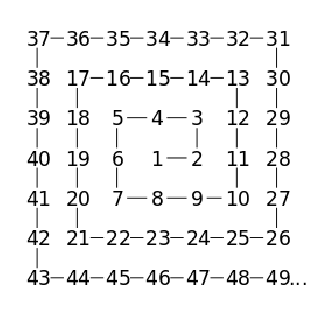
\includegraphics{spiral5}
   
\item
  Дана матриця розміру $n \times m$. Поміняти місцями стовпці, що містять
  мінімальний і максимальний елементи матриці.
\item
  Дано дві матриці $n \times m$ і $m \times k$. Отримайте їх добуток.
\item
  Дана матриця розміру $n \times m$. Поміняти місцями її рядки так, щоб їх
  максимальні елементи утворювали зростаючу послідовність.
\item
  У даній дійсної квадратної матриці порядку $n$ знайти найбільший по
  модулю елемент.
\item
  Отримати квадратну матрицю порядку $n - 1$ шляхом викидання з вихідної
  матриці будь-якого рядка і стовпця, на перетині яких розташований
  елемент зі знайденим значенням. Виконуйте до тих пір, поки не
  залишиться останній елемент.
\item
  Дана квадратна матриця порядку $2n + 1$. Дзеркально відобразити її
  елементи відносно побічної діагоналі матриці.
\item
  Дана дійсна квадратна матриця порядку $2n + 1$. Отримати нову матрицю,
  повернувши її блоки, обмежені діагоналями, на 90 градусів.
\item
  Дана матриця розміру $n \times m$. Поміняти місцями її перший і останній
  рядки, що містять тільки негативні елементи.
\item
  Дана цілочисельна матриця розміру $n \times m$. Знайти елемент, який є
  максимальним у своєму рядку і мінімальним в своєму стовпці. Якщо такий
  елемент відсутній, то вивести 0.
\item
  Складіть програму циклічної перестановки стовпців двовимірного масиву
  $n \times m$, при якій зсуві зсувається вправо на $k$ стовпців.
\item
  Дана матриця розміру $n \times m$. Поміняти місцями її стовпці так, щоб їх
  мінімальні елементи утворювали зростаючу послідовність.
\item
  Дана квадратна матриця порядку $2n + 1$. Дзеркально відобразити її
  елементи відносно вертикальної осі симетрії матриці.
\item
  Дана квадратна матриця порядку $2n$. Повернути її на 270 градусів в
  додатньому напрямку щодо її центру.
\item
  Дана матриця розміру $n \times m$. Поміняти місцями рядки, що містять
  мінімальний і максимальний елементи матриці.
\item
  У квадратній таблиці обміняйте місцями елементи рядка і стовпця, на
  перетині яких знаходиться мінімальний з позитивних елементів.
\item
  Дана квадратна матриця порядку $2n$. Повернути її на 90 градусів в
  за годинниковою стрілкою щодо її центру.
\item
  Дана квадратна матриця порядку $2n + 1$. Дзеркально відобразити її
  елементи відносно головної діагоналі матриці.
\item
  Складіть програму циклічної перестановки рядків двовимірного масиву $n \times m$,
  при якій зсув відбувається вниз на $k$ рядків.
\item
  Дана матриця розміру $n \times m$. Поміняти місцями її перший і останній
  стовпці, що містять тільки позитивні елементи.
\item
  Заповнити двовимірний квадратний масив цілими числами від 1 до 100 по
  спіралі, починаючи від центру і закручуючи за годинниковою стрілкою.
\item
  Заповніть квадратну матрицю $n \times n$ за принципом латинського квадрата: в
  кожному рядку і кожному стовпці використовуються лише числа від 1 до n
  що не повторюються між собою.
\item
  Дана матриця дійсних коефіцієнтів. Впорядкувати її рядки по неспаданню
  перших елементів, суми значень рядків, величині найменших елементів
  рядків.
\item
Знайдіть квадратну матрицю, зворотну даної з розміром n x n.
\item
Дана квадратна матриця порядку 2n. Повернути її на 180 градусів в
позитивному напрямку.
\item
Дана матриця розміру n x m. Поміняти місцями стовпці, що містять
мінімальний і максимальний елементи матриці.
\item
Дано дві матриці n x m і m x k. Отримайте їх добуток.
\item
Дана квадратна матриця порядку 2n + 1. Дзеркально відобразити її
елементи відносно побічної діагоналі матриці.
\item
Дана дійсна квадратна матриця порядку 2n + 1. Отримати нову матрицю,
повернувши її блоки, обмежені діагоналями, на 180 градусів.
\item
Дана матриця розміру n x m. Поміняти місцями її перший і останній рядки,
що містять тільки негативні елементи.
\item
Дана цілочисельна матриця розміру n x m. Знайти елемент, який є
максимальним у своєму рядку і мінімальним в своєму стовпці. Якщо такий
елемент відсутній, то вивести 0.
\item
Складіть програму циклічної перестановки стовпців двовимірного масиву m
x k, при якій зсуві зсувається вправо на n стовпців.
\item
Дана матриця розміру n x m. Поміняти місцями її стовпці так, щоб їх
мінімальні елементи утворювали зростаючу послідовність.
\item
Дана квадратна матриця порядку 2n + 1. Дзеркально відобразити її
елементи відносно вертикальної осі симетрії матриці.
\item
Дана квадратна матриця порядку 2n. Повернути її на 270 градусів в
позитивному напрямку щодо її центру.
\item
Дана матриця розміру n x m. Поміняти місцями рядки, що містять
мінімальний і максимальний елементи матриці.
\item
Дана квадратна матриця порядку 2n + 1. Дзеркально відобразити її
елементи відносно головної діагоналі матриці.
\item
Складіть програму циклічної перестановки рядків двовимірного масиву m x
k, при якій зсув відбувається вниз на n рядків.
\item
Дана матриця розміру n x m. Поміняти місцями її перший і останній
стовпці, що містять тільки позитивні елементи.
\item
Дана матриця дійсних коефіцієнтів. Впорядкувати її рядки по неспаданню
перших елементів, суми значень рядків, величині найменших елементів
рядків.
\end{enumerate}

\section{Виділення пам'яті, вказівники та рядки}

\subsection{Вказівники та виділення пам'яті}

\begin{enumerate}

\item
\item
  Ввести натуральне число $n$. Створити та ввести масив з $n$ дійсних чисел та
  підрахувати суму квадратів елементів цього масиву. 

\item
  Написати функцію, що вводить масив цілих чисел доки не введеться нуль
  через змінний аргумент та кількість елементів масиву повертається як
  результат роботи функції. Кількість елементів обмежена числом 100.
  Підрахувати кількість повних квадратів та кубів в цьому масиві.
\item
  Створити функцію, що вводить $n$-вимірний вектор($n$
  задається як аргумент функції), виділяючи відповідну
  пам'ять та функцію, що відповідно очищує пам'ять. Напишіть програму,
  що вводить два вектори, підраховує та створює як окремий масив їх
  різницю якщо це можливо, та в будь-якому варіанті коректно
  завершує програму без витоків пам'яті.
\item
  Створити функції, що коректно ініціалізують нулями та вводять з консолі 
дійсну квадратну $n$-вимірну матрицю ($n$ задається як аргумент функції), й
  функцію, що відповідно очищує пам'ять. Напишіть програму, що вводить
  дві матриці, підраховує та обчислює як окремий масив їх добуток, якщо
  це можливо, та в будь-якому варіанті коректно завершує програму без
  витоків пам'яті. Зробіть дану задачу:
  \begin{itemize}
  \item
представляючі матрицю у вигляді двовимірного масиву;
  \item
представляючі матрицю у вигляді лінійного масиву розміру $n^{2}$.
 \end{itemize}

\item
  Створити функцію, що вводить матрицю цілих чисел довільних
  розмірностей, виділяючи відповідну пам'ять (розміри масивів) та
  функцію, що відповідно очищує пам'ять. Напишіть функцію, що підраховує
  ранг матриці. Коректно протестуйте роботу цих функцій.
\item
  Створити функцію, що вводить матриці довільних розмірностей, виділяючи
  відповідну пам'ять та функцію, що відповідно очищує пам'ять. Напишіть
  програму, що вводить масив таких матриць, підраховує та створює як
  окремий масив добуток всього масиву матриць, якщо це можливо, та в
  будь-якому варіанті коректно завершує програму без витоків пам'яті.

\item
  Ввести натуральне число $n$. Створити та ввести масив з $n$ натуральних
 довгих чисел та підрахувати кількість ступенів двійки та трійки в цьому масиві.
\item
  Вирішіть завдання виконуючи наступні вимоги:

Сформувати динамічний двовимірний дійсний масив $N \times M$, заповнити його випадковими
числами або з консолі та вивести на екран. Виконати наступні дії, коректно оброблюючи 
всі можливі сценарії:

\begin{enumerate}[label=\xslalph*)]
\item
  додати рядок після заданого номеру $k$;
\item
  додати стовпець після заданого номеру $k$;
\item
  додати рядок в кінець матриці;
\item
  додати стовпець в кінець матриці;
\item
  додати рядок в початок матриці;
\item
  додати стовпець в початок матриці;
\item
  додати $k$ рядків в кінець матриці;
\item
  додати $k$ стовпців в кінець матриці;
\item
  додати $k$ рядків в початок матриці;
\item
  додати $k$ стовпців в початок матриці;
\item
  видалити рядок з номером $k$;
\item
  видалити стовпець з номером $k$;
\item
  видалити рядки, починаючи з рядка $k1$ і до рядка $k2$;
\item
  видалити стовпці, починаючи з стовпця $k$ і до стовпчика $k$;
\item
  видалити всі непарні рядки;
\item
  видалити всі парні стовпці;
\item
  видалити всі рядки, в яких є хоча б один нульовий елемент;
\item
  видалити всі стовпці, в яких всі елементи менші за 1;
\item
  видалити рядок, в якій знаходиться наймеший за модулем елемент матриці (
якщо їх декілька -- видалити усі);
\item
  додати рядок після кожного парного рядку матриці;
\item
  додати стовпець після кожного парного стовпця матриці;
\item
  додати $k$ рядків, починаючи з рядку за номером $m$;
\item
  додати $k$ стовпців, починаючи зі стовпчика за номером $m$;
\item
  додати рядок після рядка, що містить найбільший елемент;
\item
  додати стовпець після стовпця, що має найбільшу суму елементів;
\item
  додати рядок після рядка, що має найменше значення норми (суми квадратів)(
якщо їх декілька -- обираємо останній);
\item
  додати стовпець після стовпця, що містить найменший за модулем елемент (
якщо їх декілька -- обираємо перший);
\item
  видалити рядок і стовпець, на перетині яких знаходиться найбільший
  елемент матриці.
\end{enumerate}

\item
  Користувачу надається можливість декілька разів вводити розмірність
  вектору дійсних чисел та самі ці значення. Після кожного вводу
  потрібно підрахувати середнє арифметичне та дисперсію всіх введених
  значень.
\item
  Петя та Вася кожен день на протязі $N$ днів вимірюють
  декілька (від 0 до 1000) разів температуру повітря (хоча інколи хтось
  може забути це зробити). Створіть програму, що дозволить їм ввести ці
  результати за кожен день спостережень та підрахує середню температуру
  кожного з цих днів, де сумарна кількість вимірювань була більше 1.
  Програма повинна передбачити, що після вводу цих $N$ днів вони можуть
  захотіти ввести наступні $M$ днів таких спостережень. Передбачте
  можливість коректного завершення при нестачі ресурсів комп'ютера для
  зберігання та обробки даних.
\item
 В масиві натуральних чисел A{[}N{]} всі числа є меншими 16. Напишить
  функцію, що зберігає дані цього масиву у масиві $N/2$ чисел типу
  uint8\_t (тобто в кожному числі uint8\_t зберігається два числа масиву
  A{[}i{]}).
\item
  В масиві натуральних чисел A{[}N{]} всі числа є меншими 64. Напишить
  функцію, що зберігає дані цього масиву у масиві $[N*4/3]$ чисел типу
  uint8\_t (тобто в кожних трьох числах uint8\_t зберігається чотири
  числа масиву A{[}i{]}).
\item
  В масиві натуральних чисел A{[}N{]} всі числа є меншими \(2^{k}\).
  Знайдіть це число $k$ та напишить функцію, що зберігає цей масив в $N*k$
  біт найбільш економічним чином( int A{[}3{]}, k=5 → uint8 B{[}2{]}
  ,тобто використовує 16 біт, або int A{[}8{]}, k=14 → uint16 B{[}7{]} ,
  тобто використовує 112 біт) та функцію що обратно повертає числа з
  масиву B у масив A.
\end{enumerate}



\subsection{ Рядки Сі (Null-terminated
strings)}
\begin{enumerate}
\item
Дано рядок, серед символів якого є принаймні одна кома, а може й
немає її. Знайти номер:
\begin{enumerate}[label=\xslalph*)]
\item першої по порядку коми;
\item останньої по порядку коми;
\item кількості ком.
\end{enumerate}

\item
Надрукувати заданий рядок:
 \begin{enumerate}[label=\xslalph*)]
 \item виключивши з нього всі цифри і подвоївши знаки '+' та '-';
 \item виключивши з нього всі знаки '+', безпосередньо за якими знаходиться
цифра;
 \item виключивши з нього всі літери '\emph{b}', безпосередньо перед якими
знаходиться літера '\emph{c}';
 \item замінивши в ньому всі пари '\emph{ph}' на літеру '\emph{f}';
 \item виключивши з нього всі зайві пропуски, тобто з кількох, що йдуть
підряд, залишити один.
\end{enumerate}

\item
Виключити з заданого рядка групи символів, які знаходяться між '(' та
')'. Самі дужки теж мають бути виключені. Перевірте перед цим, що дужки
розставлено правильно (парами) та всередині кожної пари дужок немає
інших дужок.

\item
Задана послідовність символів, яка має вигляд:\\
\emph{d\textsubscript{1}} ± \emph{d\textsubscript{2}} ± \emph{...} ±
\emph{d\textsubscript{n }} ($n \ge 1 $, а текст \emph{d\textsubscript{i }} -- це натуральні
числа), за якою знаходиться знак рівності.
Напишить функцію, яка перевряє що рядок задовольняє вказаний вигляд та обчислити значення
цієї алгебраїчної суми. В противному випадку повернути найменше можливе ціле число.

\item
Задане натуральне число $n$ ($n<100$). Надрукувати в заданій системі числення $b$ ($1<b<17$)
цілі числа від 0 до $n$.

\item Заданий рядок, серед символів якого міститься двокрапка ':'.
 Отримати всі символи, розташовані:
\begin{enumerate}[label=\xslalph*)]
\item до першої двокрапки включно;
\item після першої двокрапки;
\item між першою і другою двокрапкою. Якщо другої двокрапки немає, 
то отримати всі символи, розміщені після єдиної двокрапки.
\end{enumerate}

\item
  Заданий текст надрукувати по рядках, розуміючи під рядком або наступні
  6 символів, якщо серед них немає коми (знак оклику, питання), або
  частину тексту до коми включно.
\item
  Знайти у даному рядку символ та довжину найдовшої послідовності
  однакових символів, що йдуть підряд.
\item
  Скласти програму підрахунку загального числа входжень символів '+',
  '-', '*' у рядок \emph{А}.
\item
  Скласти програму перетворення рядка \emph{А}, замінивши у ньому всі
  знаки оклику '!' крапками '.', кожну крапку -- трьома крапками '...',
  кожну зірочку '*'-- знаком '+'.
\item
  Рядок називається симетричним, якщо його символи, рівновіддалені від
  початку та кінця рядка, співпадають. Порожній рядок вважається
  симетричним. Перевірити рядок \emph{A} на симетричність.
\item
  Скласти програму видалення із рядка \emph{А} всіх входжень заданої
  групи символів.
\item
  Скласти програму перетворення слова \emph{А}, видаливши у ньому кожний
  символ '*' та подвоївши кожний символ, відмінний від '*'.
\item
  Скласти функцію підрахунку найбільшої кількості цифр, що йдуть підряд
  у рядку \emph{А}.
\item
  Скласти функція підрахунку числа входжень у рядок \emph{А} заданої
  послідовності літер.
\item
  Скласти функцію, яка за рядком \emph{А} та символом \emph{s} будує
  новий рядок, отриманий заміною кожного символу, наступного за
  \emph{s}, заданим символом \emph{c}.
\item
  Cкласти функцію перетворення рядка \emph{А} видаленням із нього всіх
  ком, які передують першій крапці, та заміною у ньому знаком '+' усіх
  цифр '3', які зустрічаються після першої крапки.
\item
  Cкласти функцію виведення на друк усіх цифр, які входять в заданий
  рядок, та окремо решти символів, зберігаючи при цьому взаємне
  розташування символів у кожній з цих двох груп.
\item
  Рядок називається монотонним, якщо він складається з зростаючої або
  спадної послідовності символів. Cкласти функцію перевірки
  монотонності рядка.
\item
За допомогою масиву рядків виведіть на екран зображення вісей координат на ділянці
[-5,5]x[-5,5] з підписами кожної вісі та точки О. Введіть дві координати (x,y) 
в цьому інтервалі та за допомогою символу „X“ виведіть знаходження цієї точки. 
Для цього створіть функції додавання точки до існуючих та перемалювання точки.

\item
  В заданий рядок входять тільки цифри та літери. Визначити, чи
  задовольняє він наступній властивості:
  \begin{enumerate}[label=\xslalph*)]
\item рядок є десятковим записом числа, кратного 9 (6, 4);
\item рядок починається з деякої ненульової цифри, за якою знаходяться
тільки літери і їх кількість дорівнює числовому значенню цієї цифри;
\item рядок містить (крім літер) тільки одну цифру, причому її числове
значення дорівнює довжині рядка;
\item сума числових значень цифр, які входять в рядок, дорівнює довжині
рядка;
\item рядок співпадає з початковим (кінцевим, будь-яким) відрізком ряду
0123456789;
\item рядок складається тільки з цифр, причому їх числові значення
складають арифметичну прогресію (наприклад, 3 5 7 9, 8 5 2, 2).
  \end{enumerate}

\item
  Перевірити, чи складається рядок з:
 \begin{enumerate}[label=\xslalph*)]
 \item 2 симетричних підрядків;
 \item $n$ симетричних підрядків (для всіх можливих $n>1$).
 \end{enumerate}

\item
  Знайти символ, кількість входжень якого у рядок \emph{A}
\begin{enumerate}[label=\xslalph*)]
  \item максимальна;
  \item мінімальна.
\end{enumerate}
\item
Дано рядок \emph{A}, що містить послідовність слів. Скласти функції, що визначають:
\begin{enumerate}[label=\xslalph*)]
\item кількість усіх слів;
\item кількість слів, що починаються із заданого символу \emph{c};
\item кількість слів, що закінчуються заданим символом \emph{c};
\item кількість слів, що починаються й закінчуються заданим символом \emph{c};
\item кількість слів, що починаються й закінчуються однаковим символом.
\end{enumerate}

\item 
  Виділити з рядка \emph{A} найбільший підрядок, перший і останній
  символи якого співпадають.
\item
  Виділити з рядка найбільший монотонний підрядок, коди послідовних
  символів якого відрізняються на 1.
\item
  Замінити всі пари однакових символів рядка, які йдуть підряд, одним
  символом. Наприклад, рядок \emph{`aabcbb'} перетворюється у
  \emph{`abcb'}.
\item
  Побудувати рядок \emph{S} з рядків \emph{S1}, \emph{S2} так, щоб у
  \emph{S} входили:
\begin{enumerate}[label=\xslalph*)]
\item ті символи \emph{S1}, які не входять у S2;
\item всі символи \emph{S1}, які не входять у \emph{S2}, та всі символи
\emph{S2}, які не входять у \emph{S1}.
\end{enumerate}

\item
Видалити з рядка симетричні початок та кінець. Наприклад, рядок
\emph{`abcdefba'} перетворюється у \emph{`cdef'}. 

\item
Написати функцію, яка виконує зсув по ключу (ключ задається) для малих 
та великих латинських літер. Наприклад: вхідні дані \emph{`Any`} -- рядок, 3 -- ключ.
Результат: \emph{`Dpq`}.

\item
  Встановити, чи задовольняє заданий рядок заданому шаблону. Шаблон ---
  це рядок, що складається з символів а також наступних спецсимволів:
  символ «?» позначає будь-який символ, «*» означає будь-яку
  послідовність символів, у тому числі порожню, а «+» будь-яку непорожню
  послідовність символів (приклад, «ab*ra??da+ra»).

\item
 Напишить функцію обчислення хешу рідку. Хеш даного рядку
 (довжина рядку більше одиниці) це ціле число, 
що відповідає рядку та обчислюється за наступними варіантами:

\begin{enumerate}[label=\xslalph*)]
\item Кожні послідовні 4 байти конкатинуються щоб утворити натуральне
число. Якщо кількість символів не кратна 4, то до рядка дописуються
потрібна кількість символів, що взята з кінця рядку справа наліво
(зеркальний падінг). Всі ці числа додаються за допомогою ``виключного
або'' (xor).
\item Кожні послідовні 4 байти конкатинуються щоб утворити натуральне
число. Якщо кількість символів не кратна 4, то до рядка дописуються
потрібна кількість нулевих символів (нульовий падінг. До всіх цих чисел
додається за допомогою ``виключного або'' номер по порядку цього числа.
Потім всі ці числа додаються за допомогою ``виключного або''.
\item Береться просте число p. Кожен послідовні байт множиться на $p^{i}$,
 де $i$ --- номер по порядку цього числа та береться
остача від ділення на $2^{32}$. Потім всі ці числа додаються по модулю $2^{32}$.
\end{enumerate}

\item
Надрукувати заданий рядок:
\begin{enumerate}[label=\xslalph*)]
\item
виключивши з нього всі цифри і подвоївши знаки '+' та '-';

\item виключивши з нього всі знаки '+', безпосередньо за якими знаходиться
цифра;
\item
 виключивши з нього всі літери 'в', безпосередньо перед якими
знаходиться літера 'с';

\item замінивши в ньому всі пари 'ph' на літеру 'f';
\item виключивши з нього всі зайві пропуски, тобто з кількох, що йдуть
підряд, залишити один.
\end{enumerate}
\item
Пересвідчитись, що заданий рядок відповідає запису сімнадцяткового числа
(цифри `a'-`g' можуть бути як великого так і маленького регістру, але
обов'язково одного того самого регістру) та вивести його у десятковому
вигляді.
\item
Знайти у даному рядку символ та довжину найдовшої послідовності
однакових символів, що йдуть підряд.
\item
Скласти програму підрахунку загального числа входжень символів '+', '-',
'*' у рядок А.
\item
Скласти програму перетворення рядка А, замінивши у ньому всі знаки
оклику '!' крапками '.', кожну крапку -- трьома крапками '...', кожну
зірочку '*'- знаком '+'.
\item
Рядок називається симетричним, якщо його символи, рівновіддалені від
початку та кінця рядка, співпадають. Порожній рядок вважається
симетричним. Перевірити рядок A на симетричність.
\item
Скласти програму видалення із рядка А всіх входжень заданої групи
символів.
\item
Скласти програму перетворення слова А, видаливши у ньому кожний символ
'*' та подвоївши кожний символ, відмінний від '*'.
\item
Скласти функцію підрахунку найбільшої кількості цифр, що йдуть підряд у
рядку А.
\item
Скласти функцію підрахунку числа входжень у рядок А заданої
послідовності літер.
\item
Скласти функцію, яка за рядком А та символом S будує новий рядок,
отриманий заміною кожного символу, що слідує за S, заданим символом С.
\item
Скласти функцію перетворення рядка А видаленням із нього всіх ком, які
передують першій крапці, та заміною у ньому знаком '+' усіх цифр '3',
які зустрічаються після першої крапки.
\item
Скласти функцію виведення на друк усіх цифр, які входять в заданий
рядок, та окремо - решту символів, зберігаючи при цьому взаємне
розташування символів у кожній з цих двох груп.
\item
Рядок називається монотонним, якщо він складається з зростаючої або
спадної послідовності символів. Скласти функцію перевірки монотонності
рядка.
\item
Перевірити, чи складається рядок з
\begin{enumerate}[label=\xslalph*)]
\item
2 симетричних підрядків;
\item n симетричних підрядків.
\end{enumerate}
\item
Знайти символ, кількість входжень якого у рядок A

а) максимальна;

б) мінімальна.
\item
Виділити з рядка A найбільший підрядок, перший і останній символи якого
співпадають.
\item
Виділити з рядка найбільший монотонний підрядок, коди послідовних
символів якого відрізняються на 1.
\item
Замінити всі пари однакових символів рядка, які йдуть підряд, одним
символом. Наприклад, рядок `aabcbb' перетворюється у `abcb'.
\item
Побудувати рядок S з рядків S1, S2 так, щоб у S входили
\begin{enumerate}[label=\xslalph*)]
\item
 ті символи S1, які не входять у S2;

\item всі символи S1, які не входять у S2, та всі символи S2, які не
входять у S1.
\end{enumerate}
\item
Видалити з рядка симетричні початок та кінець. Наприклад, рядок
`abcdefba' перетворюється у `cdef'.

\item
Введіть 5 різних дійсних чисел та виведіть їх послідовно в різних
рядках, так щоб відстань від лівого краю екрану до кожного числа
дорівнювала значенню цифри найстаршого розряду числа:

1.0

0.4

4.6578

6.144

2.56

За допомогою масиву рядків виведіть на екран зображення вісей координат
на ділянці {[}-5,5{]}x{[}-5,5{]} з підписами кожної всі та точки О.
Введіть дві координати (x,y) в цьому інтервалі та за допомогою символу
„X`` виведіть знаходження цієї точки. Для цього створіть функції
додавання точки до існуючих та перемалювання точки.
\end{enumerate}

\subsection{ Локалізація рядків}
\begin{enumerate}
\item
Реалізувати функцію виведення на друк тільки маленьких літер
українського алфавіту, які входять в заданий рядок.
\item
Заданий рядок, який складається з великих літер українського алфавіту.
Скласти програму перевірки впорядкованості цих літер за алфавітом.
\item
Дано натуральне число \(n\), символ \(s\)
(\(n \leq 1000\),\(\text{s\ }\)- одна з букв і, р, д, в, т, п, яка
вказує відмінок -називний, родовий, давальний, знахідний, орудний,
місцевий, окличний). Записати кількісний числівник, що означає запис
числа \(n\) у відповідному відмінку.

\end{enumerate}

\section{Файли}

\subsection{ Символьні файли (файли, що містять послідовності символів)}

\begin{enumerate}
\item
Дано символьний файл F. Побудувати файл G, утворений з файлу F:
\begin{enumerate}[label=\xslalph*)]
\item зміною всіх його великих літер однойменними малими;

\item  записом його компонент у зворотному порядку.
\end{enumerate}
\item
Дано символьний файл, що складається не менш ніж із 2 компонент.
Визначити, чи є два перших символи файлу цифрами. Якщо так, то виявити,
чи є число, утворене цими цифрами, парним.
\item
Задано символьні файли F і G. Записати до файлу H спочатку 
компоненти файлу F, потім -- файлу G зі збереженням порядку.

\item
Дано символьний файл. Скласти підпрограми для:
\begin{enumerate}[label=\xslalph*)]
\item
додавання в його кінець заданого символу;
\item
додавання в його початок заданого символу;
\item
підрахунку кількості входжень до файлу заданого символу;
\item
визначення входження до файлу заданої комбінації символів;
\item
вилучення заданого символу;
\item
вилучення інших входжень кожного символу.
\end{enumerate}
\item
Скласти функцію перевірки рівності файлів, виконаної за один перегляд
їхнього змісту. Символьні файли рівні, коли вони складаються з тих самих
слів в тому ж порядку. Слова відокремлюються одним чи більше пробілами.

\item
Дано символьний файл. Групи символів, що відокремлені пропусками (одним
або кількома) і не містять пропусків усередині, називатимемо словами.
Скласти підпрограми для:
\begin{enumerate}[label=\xslalph*)]
\item
знаходження найдовшого слова у файлі;
\item
визначення кількості слів у файлі;
\item
вилучення з файлу зайвих пропусків і всіх слів, що складаються з
однієї літери;
\item
вилучення всіх пропусків на початку рядків, у кінці рядків і між
словами (крім одного);
\item
вставки пропусків до рядків рівномірно між словами так, щоб довжина
всіх рядків (якщо в них більше 1 слова) була 80 символів і кількість
пропусків між словами в одному рядку відрізнялась не більш ніж на 1
(вважати, що рядки файлу мають не більш ніж 80 символів).
\end{enumerate}
Результат записати до файлу H.
\item

Підрахувати кількість слів в даному символьному файлі, які починаються з
даної послідовності літер. Врахуйте можливість перенесення складів
одного слова в різні рядки

\end{enumerate}

\subsection{ Текстові файли}

\emph{Організуйте роботу з текстовим
файлом. Вихідні файли не передбачають зміни. Змінені дані збережіть в
іншому файлі.}

\begin{enumerate}
\item
Дано два текстові файли з іменами Name1 і Name2. Додати в кінець кожного
рядка файлу Name1 відповідний рядок файлу Name2. Якщо файл Name2
коротший файлу Name1, то виконайте перехід до початку файлу Name2.
\item
Організувати текстовий файл, що складається з N рядків. Визначити
максимальний і мінімальний розмір рядків в файлі і вивести їх в інший
файл.
\item
Дан текстовий файл з ім'ям NameT. Підрахувати число повторень в ньому
малих латинських літер ('a' - 'z') і створити файл з ім'ям NameS, рядки
якого мають вигляд: "\textless{}літера\textgreater{} - \textless{}число
повторень даної літери\textgreater{}". Літери, відсутні в тексті, в файл
не включати. Рядки впорядкувати за спаданням кількості повторень літер,
а при однаковій кількості повторень - по зростанню кодів літер.
\item
Дан символ с (прописна латинська літера) і текстовий файл. Створити
текстовий файл, який містить всі слова з вихідного файлу, що починаються
цією літерою (як великої, так і малої). Розділові знаки, розташовані на
початках і в кінцях слів, не враховувати. Якщо вихідний файл не містить
відповідних слів, залишити результуючий файл порожнім.
\item
У відсортоване файл прізвищ додати нове прізвище, не порушивши його
впорядкованість.
\item
Дан текстовий файл. Створити файл, що містить всі символи, які
зустрілися в тексті, включаючи пробіл і знаки пунктуації (без
повторень). Символи розташовувати в порядку зростання їх кодів.
\item
Організувати текстовий файл f що складається з N рядків. Після цього
організувати файли h і g., де у файлі h записуються рядки файлу f які
займають непарні позиції, а в файлі g парні.
\item
Дан текстовий файл f. Створити файл g, що містить всі символи, які
зустрілися в тексті, включаючи пробіл і знаки пунктуації (без
повторень). Символи розташовувати в порядку проходження у вихідному
файлі.
\item
Дано ціле число N і текстовий файл з ім'ям Name1, що містить один абзац
тексту, вирівняний по лівому краю. Відформатувати текст так, щоб його
ширина не перевищувала N позицій, і вирівняти текст по лівому краю.
Прогалини в кінці рядків видалити. Зберегти відформатований текст в
новому текстовому файлі з іменемName2.
\item
Організувати текстовий файл f, що складається з N рядків. Організувати
заміну символів в файлі. "Старий" символ і "новий" символ запитуються і
вводяться з клавіатури. Зміна вивести в другий файл.
\item
Дан текстовий файл. Вивести в інший файл найдовші слова тексту (з
урахуванням розділових знаків, розташованих на початку та в кінці слів).
\item
Додати в вказане місце файлу задану кількість рядків, починаючи з
зазначеного місця іншого файлу. Місце задається номером рядка. Результат
вивести в третій файл.
\item
У файлі зберігаються назви товарів і ціни в гривнях 1997 р Створити
новий файл, перетворивши ціни товару в рублі і копійки 1998 року,
додавши найменування "грн." і "коп.". У зазначений рік ціни зменшилися в
1000 разів.
\item
Видалити задану кількість рядків із зазначеного місця файлу. Зміни
вивести в другий файл. Якщо дію неможливо, вивести про це повідомлення
на екран і в вихідний файл
\item
Організувати текстовий файл f, що складається з N рядків. Після цього
створити текстовий файл g, що містить рядки текстового файлу f в
зворотному порядку.
\item
Дан файл, який містить текст, вирівняний по лівому краю (довжина кожного
рядка не перевищує 50 символів). Вирівняти його по правому краю, додавши
в початок кожної непорожній рядки необхідну кількість прогалин.
Вирівняний текст записати в інший файл.
\item
Організувати текстовий файл, що складається з N рядків. Вивести на екран
і в інший файл рядки, розмір яких більше середнього розміру рядка в
файлі.
\item
Дан текстовий файл. Створити файл, що містить всі знаки пунктуації, які
зустрілися в текстовому файлі в тому ж порядку.
\item
Організувати текстовий файл, що складається з N рядків. Замінити в файлі
все маленькі латинські літери на великі і вивести це в інший файл.
\item
Дан текстовий файл. Вивести в інший файл найкоротші слова тексту (з
урахуванням розділових знаків, розташованих в кінці слів). Коротке слово
не є порожнім.
\item
Організувати текстовий файл, що складається з N рядків. Замінити в ньому
все рядки даної довжини новим рядком. Довжину замінних рядків і вміст
нового рядка запитується і вводиться з клавіатури. Якщо таких рядків
немає, то дані не змінювати. Зміна вивести в новий файл.


\emph{Організуйте роботу з текстовим
файлом. Вхідний файл потрібно змінити згідно вказаних умов, тобто
вхідний та вихідні файли співпадають.}

\item
Дано число N і текстовий файл. Видалити з файлу рядки з номерами,
кратними N. Порожні рядки не враховувати і не видаляти. Якщо рядки з
необхідними номерами відсутня, то залишити файл без змін. Зміна вивести
в другий файл.
\item
Дан текстовий файл, що містить текст, вирівняний по лівому краю (довжина
кожного рядка не перевищує 50 символів). Вирівняти його по центру,
додавши в початок кожної непорожній рядки необхідну кількість прогалин.
Рядки непарної довжини перед центруванням доповнювати зліва прогалиною.
Вирівняний текст записати в інший файл.
\item
Організувати текстовий файл, що складається з N рядків. Перетворити
файл, видаливши в кожній його рядку зайві пробіли. Зміни вивести в
другий файл.
\item
Дан файл з текстом із символів латинського алфавіту. Зашифрувати файл,
виконавши циклічний зсув кожної букви вперед на n позицій в алфавіті.
Розділові знаки і пропуски не змінювати.
\item
Дано числа N1, N2 і текстовий файл. Видалити з файлу рядки з номерами
між N1, N2, не включаючи меж. Зміни вивести в другий файл. Якщо виконати
видалення неможливо, видайте про це повідомлення на екран і в вихідний
файл.
\item
Дан файл з текстом із символів латинського алфавіту, цифр та знаків.
Замініть всі цифри їх назвами на англійській мові.
\item
Організувати текстовий файл f складається з N рядків. Після цього
організувати файли h і g. У файл h записати рядки файлу f непарної
довжини, в файл g парної довжини.
\item
Визначити функцію, яка:
\begin{enumerate}[label=\xslalph*)]
\item підраховує кількість порожніх рядків;

\item обчислює максимальну довжину рядків текстового файлу.
\end{enumerate}

\item
Визначити процедуру виведення:
\begin{enumerate}[label=\xslalph*)]
\item усіх рядків текстового файлу;

\item рядків, які містять більше 60 символів.
\end{enumerate}

\item
 Визначити функцію, що визначає кількість рядків текстового файлу,
які:
\begin{enumerate}[label=\xslalph*)]
\item починаються із заданого символу;

\item закінчуються заданим символом;

\item починаються й закінчуються одним і тим самим символом;

\item що складаються з однакових символів.
\end{enumerate}

\item
В даному текстовому файлі знаходиться англомовний текст. Вирівняйте його
по лівий та правий границі так щоб розподіл слів у рядках був найбільш
рівномірним.
\item
Визначити процедуру, яка переписує до текстового файлу G усі рядки
текстового файлу F:

а) із заміною в них символу '0' на '1', і навпаки;

б) в інвертованому вигляді.
\item
Визначити процедуру пошуку найдовшого рядка в текстовому файлі. Якщо
таких рядків кілька, знайти перший із них.
\item
Визначити процедуру, яка переписує компоненти текстового файлу F до
файлу G, вставляючи до початку кожного рядка один символ пропуску.
Порядок компонент не має змінюватися.
\item
У текстовому файлі записано непорожню послідовність дійсних чисел, які
розділяються пропусками. Визначити функцію обчислення найбільшого з цих
чисел.
\item
У текстовому файлі F записано послідовність цілих чисел, які
розділяються пропусками. Визначити процедуру запису до текстового файлу
g усіх додатних чисел із F.
\item
У текстовому файлі кожний рядок містить кілька натуральних чисел, які
розділяються пропусками. Числа визначають вигляд геометричної фігури
(номер) та її розміри. Прийнято такі домовленості:
\begin{itemize}
\item
відрізок прямої задається координатами своїх кінців і має номер 1;
\item
прямокутник задається координатами верхнього лівого й нижнього
\item
правого кутів і має номер 2;
\item
коло задається координатами центра й радіусом і має номер 3.
\end{itemize}

Визначити процедури обчислення:
\begin{enumerate}[label=\xslalph*)]
\item
відрізка з найбільшою довжиною;

\item прямокутника з найбільшим периметром;

\item кола з найменшою площею.
\end{enumerate}

\item
У файлі записані координати точок на площині задані парою цілих чисел.
Точки записуються в форматі: (х1, х2) (х1, х2), \ldots{} - саме так
через коми та дужки. Створити файл, в якому будуть записані координати
всіх відрізків з точок цього файлу, при цьому ці відрізки відсортовані
за зростанням довжини.
\item
У файлі записані координати Точок в просторі задані трійкою цілих чисел.
Точки записуються в форматі: х1, х2, х3; х1, х2, х3; \ldots{} Знайти
відрізок з точок цього файлу, що має найбільшу довжину.
\item
У файлі записані координати матеріальних точок на площині задані парою
цілих чисел та масою(дійсне число). Точки записуються в форматі: {[}х1 ,
y1, m1 {]}, {[}х2 , y2, m2{]} , \ldots{} - саме так через коми та дужки.
Знайдіть дві точки з найбільшим важілем сили (m*(х +y)).
\item
У файлі записані дати, що задані трійкою цілих чисел у форматі
(чч1./мм1/рр1),(чч2./мм2/рр2), \ldots{} - саме в такому форматі.
Створити файл, в якому будуть записано найстарша та найсвіжіша дати
(врахуйте, що роки дат з 1951 по 2049).
\item
У файлі записані дати , що задані двома цілими числами та рядком
(англійські назви місяця) у форматі: чч1 місяць1 рік1; чч1 місяць1
рік1;\ldots{} Знайти різницю в днях між найстаршою та найсвіжішою датою.
\item
Відомості про учня складаються з його імені, прізвища та назви класу
(рік навчання та літери), в якому він вчиться. Дано файл, який містить
відомості про учнів школи. Скласти підпрограми, які дозволяють:
\begin{enumerate}[label=\xslalph*)]
\item
 визначити, чи є в школі учні з однаковим прізвищем;

\item визначити, чи є учні з однаковим прізвищем у паралельних класах;

\item визначити, чи є учні з однаковим прізвищем у певному класі;

\item відповісти на питання а)-в) стосовно учнів, у яких збігаються ім'я та
прізвище;

\item визначити, в яких класах налічується більше 35 учнів;

\item визначити, на скільки учнів у восьмих класах більше, ніж у десятих;

\item зібрати у файл відомості про учнів 9-10-х класів, розташувавши
спочатку відомості про учнів класу 9 а, потім -- 9 б тощо;

\item отримати список учнів даного класу за зразками:

Прізвище Ім'я

Прізвище І.

І.Прізвище.
\end{enumerate}

\item
Дано файл, який містить ті самі відомості про учнів школи, що й в
попередній задачі, і додатково оцінки, отримані учнями на іспитах із
заданих предметів. Скласти процедури для:
\begin{enumerate}[label=\xslalph*)]
\item
визначення кількості учнів, які не мають оцінок, нижче 4;

\item побудови файлу, який містить відомості про кращих учнів що мають
оцінки, не нижче 4;

\item друкування відомостей про учнів, які мають принаймні одну довільну
оцінку, у вигляді прізвища та ініціалів, назви класу, предмету та
оцінки.
\end{enumerate}

\item
Відомості про автомобіль складаються з його марки, номеру та прізвища
власника. Дано файл, який містить відомості про кілька автомобілів.
Скласти процедури знаходження:
\begin{enumerate}[label=\xslalph*)]
\item
 прізвищ власників номерів автомобілів певної марки;

\item кількості автомобілів кожної марки.
\end{enumerate}

\item
Дано файл, який містить відомості про книжки. Відомості про кожну книгу
-- це прізвище автора, назва та рік видання. Скласти процедури пошуку:
\begin{enumerate}[label=\xslalph*)]
\item
 назв книг певного автора, виданих із 1960 р.;
\item
 книг із заданою назвою. Якщо така книжка є, то надрукувати прізвища
авторів і рік видання.
\end{enumerate}

\item
Дано файл, який містить номери телефонів співробітників установи:
вказуються прізвище співробітника, його ініціали та номер телефону.
Визначити процедуру пошуку телефону співробітника за його прізвищем та
ініціалами.
\item
Дано файл з відомостями про кубики: розмір кожного (довжини ребра у см),
його колір (червоний, жовтий, зелений, синій) і матеріалу (дерев'яний,
металевий, картонний). Скласти процедури пошуку:
\begin{enumerate}[label=\xslalph*)]
\item кількості кубиків кожного з перелічених кольорів, їх сумарний об'єм

\item кількості дерев'яних кубиків із ребром 3 см і металевих кубиків
ребром, більшим за 5 см.
\end{enumerate}

\item
Відомості про учнів (ПІБ, клас, дата народження) записуються до файлу
певного формату. Створіть функції для запису та редагування даних у
файлі.

Напишіть функцію, що записує в окремий файл в тому ж форматі учнів, що
містять всі оцінки більше 10.

Формат файлу:
\begin{enumerate}[label=\xslalph*)]
\item
JSON
\item
CVS
\item
XML
\end{enumerate}

\item
Відомості про предмет (Викладач, класи якім він викладається, час
читання) записуються до файлу певного формату. Створіть функції для
запису та редагування даних у файлі. Напишіть функцію, що записує в
окремий файл сумарну кількість годин для кожного викладача.
Формат файлу:
\begin{enumerate}[label=\xslalph*)]
\item
JSON
\item
CVS
\item
XML
\end{enumerate}

\item
Використовуючи дані з попередніх двох задач, напишіть функцію, що
записує в окремий файл середню оцінку кожного учня.

Формат файлу:
\begin{enumerate}[label=\xslalph*)]
\item
JSON
\item
CVS
\item
XML
\end{enumerate}


\end{enumerate}

\subsection{Робота з файлами}

\begin{enumerate}
\item
В даній директорії з підкаталогами відшукати всі файли з розширенням *.с
та поміняти їх на відповідні файли з розширенням *.срр
\item
В даній директорії з підкаталогами відшукати всі файли з розширенням
*.cpp та поміняти там коментарі вигляду // (до кінця рядку) на коментарі
де на початку рядку /* \ldots{} та в кінці рядку */
\item
В даній директорії з підкаталогами відшукати всі файли з розширенням
*.txt які модифіковані раніше заданої дати та видалити їх
\item
В даній директорії з підкаталогами відшукати всі файли з розширенням
*.txt які створені раніше ніж рік тому та перенести їх в іншу (задану)
директорію
\item
В даній директорії з підкаталогами відшукати всі файли з розширеннями
Word які менше 10 мб та замінити їх видаляє їх.
\item
Створити форму яка дозволяє ввести шлях до директорії та виводить
середній розмір текстових файлів у цій директорії.

\end{enumerate}

\subsection{ Статичні та глобальні змінні}

Розв'язати ці задачі використовуючи глобальні змінні та розв'язати ці
задачі використовуючи статичні змінні. Чим відрізняються версії програм
з глобальним та локальними змінними?
\begin{enumerate}
\item
Реалізуйте функцію, яка виводить повідомлення скільки разів вона була
викликана з головної функції до кожного з цих викликів. В імплементації
головний функції зробіть так щоб користувач мав можливість викликати цю
функцію скільки завгодно разів (наприклад, вводив кількість викликів)
\item
Реалізуйте дві функції зі змінним аргументом: перша додає до аргументу
1, друга ділить його націло на 2. Після кожного виклику однієї з цих
функцій в головній програмі повинно виводитись повідомлення, яка з цих
функцій викликалась частіше.
\item
Реалізуйте функцію, що може викликатись не більше фіксованої кількості
разів. Ця кількість разів вводиться в головній програмі або через
командний рядок.

\end{enumerate}

\section{Структури}

\subsection{ Описи структури}
\begin{enumerate}
\item
Визначити типи структури для зображення наступних понять та функції їх
вводу-виводу:
\begin{enumerate}[label=\xslalph*)]
\item ціна (гривні, копійки);

\item час (година, хвилина, секунда);

\item дата (число, місяць, рік);

\item адреса (місто, вулиця, будинок, квартира);

\item семінар (предмет, викладач, № групи, день тижня, години занять,
аудиторія);

\item бланк вимоги на книгу (відомості про книгу: шифр, автор, назва;
відомості про читача: № читацького квитка, прізвище; дата замовлення);

\item поле шахової дошки (напр., а5, b8);

\item коло (радіус, координати центра);

\item прямокутник зі сторонами, паралельними осям координат (Точка А, Точка
Б). Точка --- дві дійсні координати;
\item
сфера в просторі;
\item
прямокутний паралеліпіпед (сторони якого паралельні осям координат);
\item
поліном довільного ступеня (дійсні коефіцієнти --- безрозмірний масив).
\end{enumerate}

\item
Використовуючи тип Поле шахової дошки описати булеву функцію, яка
перевіряє, чи може ферзь за один крок перейти з одного заданого поля
шахової дошки на інше задане поле.
\item
Визначимо тип Rational (Раціональне число) як:

typedef struct \{

int numerator; // чисельник

unsigned int denominator; // знаменник

\} Rational;

Визначити функції для:
\begin{itemize}

\item обчислення суми двох раціональних чисел;
\item обчислення добутку двох раціональних чисел;
\item порівняння двох раціональних чисел;
\item зведення раціонального числа до нескоротного виду.
\end{itemize}

\item
Використовуючи опис типу Дата, визначити функції обчислення:

а) дати вчорашнього дня;

б) дня тижня за його датою в поточному році.
\item
Задано масив розмірності N, компонентами якого є структури, що містять
відомості про вершини гір. У відомостях про кожну вершину вказуються
назва гори та її висота. Визначити функції введення/виведення гір та
функції пошуку назви найвищої вершини та виведення висоти вершини з
заданою назвою (якщо вершини з такою назвою немає в масиви --- вивести
відповідне повідомлення).
\item
Відомо вартість і "вік" кожної з N моделей легкових автомобілів.
Визначити середню вартість автомобілів, вік яких більший за 5 років.
\item
Відомо інформацію про ціну та наклад кожного з N журналів. Знайти
середню вартість журналів, наклад яких менший за 10000 примірників.
\item
Відомі дані про масу й об'єм N предметів, виготовлених із різних
матеріалів. Знайти предмет, густина матеріалу якого найбільша.
\item
Відомі дані про чисельність населення (у мільйонах жителів) та площі N
держав. Знайти країну з мінімальною щільністю населення.
\item
Задано масив С розмірності N, компонентами якого є відомості про
мешканців деяких міст. Інформація про кожного мешканця містить його
прізвище, назву міста, місцеву адресу у вигляді вулиці, будинку,
квартири. Визначити процедуру пошуку двох будь-яких жителів, що мешкають
у різних містах за однаковою адресою.
\item
Відомо дані про вартість кожного з N найменувань товарів: кількість
гривень, кількість копійок. Скласти підпрограми пошуку:
\begin{enumerate}[label=\xslalph*)]
\item найдешевшого товару в магазині;

\item найдорожчого товару в магазині;

\item товару, вартість якого відрізняється від середньої вартості товару
в магазині не більш ніж на 5 гривень.
\end{enumerate}

\item
Задано масив Р розмірності N, компонентами якого є записи,
що містять анкети службовців деякого закладу. У кожній анкеті вказується
прізвище та ім'я службовця, його стать, дата народження у вигляді числа,
місяця, року. Визначити підпрограми пошуку:
\begin{enumerate}[label=\xslalph*)]

\item посади, яку обіймає найбільша кількість співробітників;

\item  співробітників з однаковими іменами;

\item  співробітників, прізвища яких починаються із заданої літери;

\item  найстаршого з чоловіків цього закладу;

\item  співробітників, вік яких менший за середній по організації;

\item  пенсійного віку (урахувати, що пенсійний вік чоловіків і жінок --
різний).
\end{enumerate}

\item
Задано масив Р, компонентами якого Рi є записи, що містять дані про
людину на ім'я i з указаного списку. Кожне дане складається зі статі
людини та її зросту. Визначити підпрограми для:
\begin{enumerate}[label=\xslalph*)]

\item обчислення середнього зросту жінок;

\item пошуку найвищого чоловіка;

\item перевірки, чи є дві людини, однакові на зріст.
\end{enumerate}
\item
Задано масив розмірності N, компоненти якого містять інформацію про
студентів деякого вишу. Відомості про кожного студента містять дані про
його прізвище, ім'я, по батькові, стать, вік, курс. Визначити процедуру
пошуку:
\begin{enumerate}[label=\xslalph*)]
\item
найпоширеніших чоловічих і жіночих імен;
\item
прізвищ та ініціалів усіх студентів, вік яких є найпоширенішим.
\end{enumerate}

\item
Задано масив розмірності N, компонентами якого є відомості про складання
іспитів студентами деякого вишу. Інформація про кожного студента задана
в такому вигляді: прізвище, номер групи, оцінка\_1, оцінка\_2,
оцінка\_3. Визначити процедуру пошуку:
\begin{enumerate}[label=\xslalph*)]
\item
студентів, що мають заборгованості принаймні з одного з предметів;
\item
 предмета, складеного найуспішніше;
\item
 студентів, що склали всі іспити на 5 і 4.
\end{enumerate}

\item
Визначити універсальний тип, який допускає зображення точки
на площині у прямокутній або полярній системі координат (3-тє поле --
тип координат). Побудувати функцію обчислення площі трикутника з
вершинами A, B, C.

\end{enumerate}

\subsection{Файли бінарні}

\begin{enumerate}
\item
Нехай множина цілих чисел задана у файлі. Визначити:
\begin{enumerate}[label=\xslalph*)]
\item
процедуру введення множини;
\item процедуру виведення множини;
\item процедуру доповнення множини;
\item процедуру видалення елемента з множини;
\item функцію, що дає відповідь, чи входить елемент до множини;
\item функцію, що дає відповідь, чи порожня множина;
\item функцію, що знаходить максимальний елемент множини;
\item функцію, що знаходить мінімальний елемент множини;
\item процедуру об'єднання множин;
\item процедуру різниці множин;
\item процедуру перетину множин;
\item функцію обчислення ваги множини;
\item функцію обчислення діаметра множини;
\item функцію, що за множиною A знаходить підмножину всіх таких її
елементів, для яких справедлива умова $Q(х)$, $x\in A$;
\item функцію, що з'ясовує, чи є множина A підмножиною множини В;
\item функцію, що з'ясовує, чи дорівнює множина A множині В.
\end{enumerate}

\item
Дано файл, компоненти якого є записи (koef, st) -- коефіцієнт і
степінь членів полінома ($koef \neq 0$). Визначити підпрограми для виконання
таких дій над поліномом:
\begin{enumerate}[label=\xslalph*)]
\item
 введення полінома;
\item
 друк полінома;
\item обчислення похідної від полінома;
\item обчислення невизначеного інтеграла від полінома;
\item упорядкування за степенями елементів полінома;
\item приведення подібних серед елементів полінома;
\item додавання, віднімання двох поліномів;
\item множення двох поліномів;
\item знаходження частки та залишку від ділення двох поліномів;
\item знаходження полінома за лінійної заміни змінної $x = dx + c$, $d \neq 0$;
\item знаходження полінома за заміни змінної $x = d/x$, $d \neq 0$;
\item знаходження ступеня поліному;
\item з'ясування, чи має поліном корені, рівні нулю, і визначення їхньої
кратності;
\item знаходження максимального за умовою Q(t) коефіцієнта серед
коефіцієнтів полінома, які задовольняють умову G(t);
\item знаходження мінімального за умовою Q(t) коефіцієнта серед
коефіцієнтів полінома, які задовольняють умову G(t);
\item знаходження значення полінома в заданій точці.
\end{enumerate}

\item
Дано файл, компоненти якого є
дійсними числами. Скласти підпрограми для обчислення:
\begin{enumerate}[label=\xslalph*)]
\item суми компонент файлу;

\item кількості від'ємних компонент файлу;

\item останньої компоненти файлу;

\item найбільшого зі значень компонент файлу;

\item найменшого зі значень компонент файлу з парними номерами;

\item суми найбільшого та найменшого зі компонент;

\item різниці першої й останньої компоненти файлу;

\item кількості компонент файлу, які менші за середнє арифметичне всіх

його компонент.
\end{enumerate}

\item
Дано файл, компоненти якого є
цілими числами. Скласти підпрограми для обчислення:
\begin{enumerate}[label=\xslalph*)]
\item  кількості парних чисел серед компонент;
\item кількості квадратів непарних чисел серед компонент;
\item різниці між найбільшим парним і найменшим непарним числами
компонент;
\item кількості компонент у найдовшій зростаючій послідовності компонент
файлу.
\end{enumerate}
\item
Дано файл F, компоненти якого є цілими числами. Побудувати файл G, який
містив би всі компоненти файлу F:
\begin{enumerate}[label=\xslalph*)]
\item
що є парними числами;
\item що діляться на 3 і на 5;
\item що є точними квадратами;
\item записані у зворотному порядку;
\item за винятком повторних входжень одного й того самого числа.
\end{enumerate}
\item
Використовуючи файл F, компоненти якого є цілими числами, побудувати
файл G, що містить усі парні числа файлу F, і файл H -- усі непарні.
Послідовність чисел зберігається.
\item
Задано натуральне число n та файл F, компоненти якого є цілими числами.
Побудувати файл G, записавши до нього найбільше значення перших n
компонент файлу F, потім -- наступних n компонент тощо. Розглянути два
випадки:
\begin{itemize}
\item кількість компонент файлу ділиться на n;
\item кількість компонент файлу не ділиться на n. Остання компонента файлу
g має дорівнювати найбільшій із компонент файлу F, які утворюють останню
(неповну) групу.
\end{itemize}
\item
Дано файл F, компоненти якого є цілими числами. Файл містить рівне число
додатних і від'ємних чисел. Використовуючи допоміжний файл H, переписати
компоненти файлу F до файлу G так, щоб у файлі G:
\begin{itemize}
\item не було двох сусідніх чисел одного знаку;

\item спочатку йшли додатні, потім -- від'ємні числа;
\item числа йшли таким чином: два додатних, два від'ємних тощо 
(припускається, що число компонент у файлі F ділиться на 4).
\end{itemize}

\item
Дано файл F, компонентами якого є записи (структури) вигляду

struct T \{

unsigned Key; // ключ

char Data{[}10{]}; // дані

\};

Такий файл називатимемо впорядкованим за ключами, якщо записи в ньому
розташовуються в порядку зростання (спадання) ключів. Скласти процедуру
пошуку запису за ключем у впорядкованому файлі. Скласти процедуру
вилучення запису із заданим ключем:

а) з впорядкованого файлу;

б) з невпорядкованого файлу.
\item
Багаж пасажира характеризується номером пасажира, кількістю речей і
їхньою загальною вагою. Дано файл пасажирів, який містить прізвища
пасажирів, і файл, що містить інформацію про багаж кількох пасажирів
(номер пасажира -- це номер запису у файлі пасажирів).

Скласти процедури для:
\begin{enumerate}[label=\xslalph*)]
\item
 знаходження пасажира, у багажі якого середня вага однієї речі 
відрізняється не більш ніж на 1 кг від загальної середньої ваги речей;

\item визначення пасажирів, які мають більше двох речей, і пасажирів
кількість речей у яких більша за середню кількість речей;

\item видачі відомостей про пасажира, кількість речей у багажі якого менша,
ніж у будь-якому іншому багажі, а вага речей -- не більша, ніж
будь-якому іншому багажі із цією самою кількістю речей;

\item визначення, чи мають принаймні два пасажири багажі, які не
відрізняються за кількістю речей і відрізняються вагою не більш ніж на 1
кг (якщо такі пасажири є, то показати їхні прізвища);

\item визначення пасажира, багаж якого складається з однієї речі вагою не
менше 30 кг.
\end{enumerate}
\item
Дано файл, який містить відомості про іграшки: указано назву іграшки
(напр., м'яч, лялька, конструктор тощо), її вартість у гривнях і вікові
межі для дітей, яким іграшка призначається (напр., для дітей від двох до
п'яти років). Скласти процедури:
\begin{enumerate}[label=\xslalph*)]
\item
пошуку назв іграшок, вартість яких не перевищує 40 грн, призначених
дітям п'яти років;
\item пошуку назв іграшок, призначені дітям і чотирьох, і десяти років;
\item пошуку назв найдорожчих іграшок (ціна яких відрізняється від ціни
найдорожчої іграшки не більш ніж на 50 грн);
\item визначення ціни найдорожчого конструктора;
\item визначення ціни всіх кубиків;
\item пошуку двох іграшок, що призначені дітям трьох років, сумарна
вартість яких не перевищує 20 грн;
\item пошуку конструктора ціною 22 грн, призначеного дітям від п'яти до
десяти років. Якщо такої іграшки немає, то занести відомості про її
відсутність до файлу.
\end{enumerate}

\item
Дано файл, який містить відомості про прямокутники: указано номер
прямокутника у файлі, координати верхнього лівого кута, нижнього правого
кута прямокутника. Скласти процедуру пошуку прямокутника з найбільшою
площею й визначення цієї площі.

\item 
У двох файлах міститься
таблиця футбольного турніру, у першому -- записано назви команд; у
другому -- результати матчів, що зберігаються у записах типу T\_Match

typedef struct \{

unsigned int n1, n2;

unsigned int b1, b2;

\} T\_Match;

Тут у структурі типу T\_Match поля n1, n2 -- номери першої і другої

команд (тобто номери назв команд у файлі команд); b1, b2 -- кількість

м'ячів, забитих першою та другою командами, відповідно.

Кожній команді за перемогу нараховується 3 очки, за нічию -- 1, за

поразку -- 0.

Із двох команд, які мають однакову кількість очок, першою вважається та,
що має кращу різницю забитих і пропущених м'ячів;

за однакової різниці має більше забитих м'ячів;

за всіма однаковими попередніми показниками визначається жеребкуванням
(для жеребкування використати генератор випадкових чисел).

Знайти команду, яка є лідером.

Вказівка. Описати підпрограми створення файлів команд і матчів,

додавання результату матчу, визначення лідера.
\item 
Файл бази даних з малюнками містить на початку ціле 32-бітне число 2051,
потім ціле 32-бітне число -- кількість малюнків, а наступні два
32-бітних числа -- кількість пікселів висоту та ширину кожного малюнку у
пікселах. При цьому ці числа задані в форматі high-indian (MSB first).
Наступний вміст файлу -- беззнакові натуральні байти (K*n*m байтів),
кожен з яких -- значення яскравостей пікселів (число від 0 до 255)
кожного з цих малюнків, що проходяться у порядку зліва-направо та
зверху-вниз.

Напишіть функцію, що перевіряє даний файл (заданий ім'ям) на
відповідність даному формату, та виводить масив яскравостей малюнка з
заданим номером, якщо такий номер та сам файл коректно задані. В
противному випадку вивести змістовне повідомлення про помилку.
\item 
Для представлення баз даних, що мітять тензори часто використовують
формат IDX (IDX file format), який має наступну форму:

magic\_number -- 32-бітове число у форматі high-indian (MSB first), в
якому перші 2 байти нулі, третій байт описує тип даних: якщо 0x08
-unsigned byte, 0x09 -- signed byte, 0x0B -- short(2 bytes), 0x0C -- int
(4 bytes), 0x0D -- float (4 bytes), 0x0E -- double (8 bytes), четвертий
байт -- кількість N розмірностей тензору;

size 1 - 32-бітове число у форматі high-indian (MSB first) величина
першої розмірності;

size 2 - 32-бітове число у форматі high-indian (MSB first) величина
другої розмірності;

**

size N - 32-бітове число у форматі high-indian (MSB first) величина N-ої
розмірності;

далі йдуть дані вказаного у першому числі формату:

data - Cі-масив даних у форматі high-indian (MSB first).

Напишіть функцію, що перевіряє даний файл (заданий ім'ям) на
відповідність даному формату, та виводить координату тензору, що задана
аргументом функції. В випадку, коли це не можливо, вивести змістовне
повідомлення про помилку.
\end{enumerate}


\subsection{Командний рядок}
\begin{enumerate}
\item
Напишіть програму, що приймає з командного рядку 1 цілий аргумент та
виведіть його квадрат. Якщо аргументів 2 або більше, або жодного --
виведіть повідомлення про помилку.
\item
Напишіть програму, що приймає з командного рядку 3 дійсних аргументи та
виводить їх середнє гармонічне. Якщо аргументів більше трьох, або менше
-- виведіть повідомлення про помилку. Якщо серед них є нуль --- інше
повідомлення про помилку.
\item
Введіть з командного рядочку ім'я текстового файлу та підрахуйте
кількість рядків в цьому файлі. Виведіть повідомлення про помилку якщо
щось негаразд.
\item
Введіть з командного рядочку ім'я декількох текстових файлів (їх повинно
бути більше одного) та підрахуйте середню щільність символів на рядок в
цих файлах.
\item
Введіть через командний рядочок наступного вигляду:

-filename name -rows rows ,

імя файлу (name) та кількість рядків (rows),

параметри -filename та -rows -- це обов'язкові літерали в рядку.

Якщо формат команди не такий як приведений вище -- виведіть повідомлення
про помилку та підказку. Якщо все вірно, створіть відповідний бінарний
файл, що містить вказану кількість цілих чисел від 0 до rows.
\item
Введіть через командний рядочок рядок наступного вигляду:

-filename name -rows rows -cols cols

імя файлу (name) та кількість рядків (rows) та стовпчиків(cols),

параметри -filename та -rows, cols -- це обов'язкові літерали в рядку.

Якщо формат команди не такий як приведений вище -- виведіть повідомлення
про помилку та підказку. Якщо все вірно, створіть відповідний текстовий
файл, що містить вказану кількість рядків заповнену cols нулями через
табуляцію.
\item
Введіть через командний рядочок рядок наступного вигляду:

-filename1 name1 -filename2 name2 -rows,

rows імя файлу (name) та кількість рядків (rows) параметри -filename1 та
-filename2, це обовязкові літерали в рядку.

А параметр -rows rows може бути необов'язковий.

Якщо формат команди не такий як приведений вище -- виведіть повідомлення
про помилку та підказку. Якщо все вірно, порівняйте чи співпадає в даних
двох файлах перші rows рядків з точністю до пробілів, якщо параметр rows
не вказаний -- файли порівнюються повністю за всіма рядками.
\item
Напишіть програму, яка приймає ціле число як аргумент командного рядка і
знаходить усі його дільники.
\item
Напишіть програму, яка приймає в якості аргументу командного рядка ім'я
текстового файлу. Відкрийте цей файл і прочитайте його по одному слову
(підказка: використовувати \textgreater{}\textgreater{}). Збережіть
кожне слово у вектор \textless{}string\textgreater{}. Примусити всі
слова в нижній регістр, відсортувати їх, видалити всі дублікати та
надрукувати результати.
\end{enumerate}

\subsection{Змінні оточення}

\begin{enumerate}
\item
Напишіть функцію, яка визначає тип операційної системи даного
комп'ютера.
\item
Напишіть функцію, яка записує вміст даного файлу в новий файл, що
знаходиться в системній директорії.
\item
Напишіть функцію, що визначає чи існує в системі змінна JAVA\_PATH, та
якщо немає, то встановлює цю змінну коректним шляхом.
\item
Напишіть функцію, що визначає чи існує в системі змінна JAVA\_PATH, а в
поточній директорії файл file1.java та якщо є, то запускає з консолі
команду `JAVA\_PATH file1.java'
\end{enumerate}

\subsection{Тип перерахування}

\begin{enumerate}
\item
Створіть та реалізуйте за допомогою перерахування базові функції
вводу-виводу для наступних сутностей:
\begin{enumerate}[label=\xslalph*)]
\item
день тижня;
\item
місяць у році;
\item
колір спектру;
\item
шахова фігура.
\end{enumerate}
\item
Опишіть тип -- структуру Card для карти з колоди для преферансу. Для
цього створіть перерахування Масть= \{Піка, Трефи, Бубна, Чирва\} та
Ранг =\{7,8,9,10, 'Jack', `Queen','King','Ace'\}. Реалізуйте логічну
функцію beat(Card x, Card y, Масть z), що вказує чи бє перша карта
другу, а третій параметр вказує яка масть є козирною.
\item
Створіть перелік величин довжини
(мм, см, дм, м, км) та реалізуйте функцію яка за введеною довжиною та
величною виміру виводить довжину в метрах.
\item
Створіть перерахування Відмінок= \{ім, бат, дат, \ldots{} \} та за
вказаним відмінком провідмінюйте задані слова -- програмування, мова,
комп'ютер.
\item
Створіть перерахування Голосні, яке містить всі англійські(українськи)
голосні та за допомогою цього типу визначить яка кількість складів в
даному реченні (вважаючи, що склад містить лише одну голосну).
\item
Створіть перерахування Course=\{N,S,W,E\} та Order=\{Forward, Back,
Left,Right\}. В нас задано початковий курс корабля та масив команд як
він рухався. Виведіть кінцевий напрямок корабля. Введіть також швидкість
судна та масив дійсних чисел, що відповідає часу -- скільки воно
рухалося за даним курсом та за допомогою цих даних визначте на яку
абсолютну відстань від початкової змістився корабель.
\end{enumerate}

\subsection{ Об'єднання}
\begin{enumerate}
\item
Визначити універсальний тип, що дозволяє представляти точку на площині в
декартовій та полярних координатах. Введіть дві точки та обчисліть
довжину відрізку на даних точках.
\item
Визначити універсальний грошовий тип, що може представляти вартість або
в гривнях та копійках, або лише в копійках з методом, що дозволяє при
цьому правильно відображати ті самі вартості.
\item
Визначити універсальний тип, що дозволяє представляти вектор в як дві
точки та як точку та вектор до другої точки. Введіть три вектори та
з'ясуйте чи колінеарні вони.
\item
Визначити універсальний тип, що дозволяє представляти точку в просторі в
декартовій, полярній та сферичних координатах. Введіть дві точки та
обчисліть довжину відрізку на даних точках.
\item
Визначити тип Пласка Фігура, що включає Круг, Квадрат, Трикутник,
Прямокутник, Трапеція. Реалізуйте функції обчислення периметру та площі
фігури.
\item
Визначте тип, що дозволяє зберігати число або будь-якого числового типу
(double, int, unsigned) або рядки «Нескінченість» та «Невизначеність».
Реалізуйте арифметичні операції для цього типу які коректно працюють з
діленням та іншими операціями для всіх можливих комбінаціях значень та
типів.
\end{enumerate}


\section {Введення-виведення С++}
\begin{enumerate}
\item
Ввести в двох різних рядках
послідовно два дійсних числа x та y та обчислити значення x в ступені y.
Результат вивести в десятковому та науковому представленні.

\item Ввести декілька (невідомо
зазделегідь скільки) дійсних числа записаних через коми та обчислити
значення функції log() для кожного з них. Якщо значення виходить за межі
області вивести слово ``None'', для інших значень результат вивести в
науковому та десятковому представленні шириною 5 символів.
\item
Три додатніх дійсні числа вводяться як рядок вигляду

А=ххх.ххх, B=xxExxx C=xxx.xxxx

Обчисліть їх середнє гармонійне та виведіть у науковому та звичайному
форматі.

\item
Ввести дійсне число від -10000 до 10000 та вивести його k-ту ступінь з
точністю до 20 знаків до десяткової коми та 4 значками після десяткової
коми.

\item
На терміналі вводяться 10*n цифр.
Перші 10 цифр -- це перше натуральне число, наступні 10 -- друге і так
далі. Введіть всі ці числа в масив розміру n та обчисліть і виведіть їх
суму (вважайте що сума влазить в точність unsigned long long ).

\item
Вивести на екран таблицю, слідкуючи, щоб виведення було рівним та
кількість цифр після коми була або 0 або 2:

+++++++++++++++ +++++++++++

+число + 1 + 2 + 3 + 4 + 5

++++++++++++++++++++++++++++

+експонента+ 1 +1.44 + 1.69 + 2

++++++++++++++++ ++++++++++

\item
Ввести з текстового файлу та з консолі натуральне число n та масиви з n
цілих чисел \(\left\{ m_{i} \right\}_{i = 1}^{n}\) та дійсних чисел
\(\left\{ x_{i} \right\}_{i = 1}^{n}\). Обчислить та виведіть у файл
числа \(\left\{ x_{i}^{m_{i}} \right\}_{i = 1}^{n}\).
\item
Вхідний потік містить набір цілих
чисел $A_i$ ($0 \le Ai \le 10^{18}$), відділений один від іншого
довільною кількістю пробілів і переводів рядків. Розмір вхідного потоку
не перевищує 256 КБ. Для кожного числа Ai, починаючи з останнього та
завершуючи першим, в окремому рядку вивести його квадратний корінь не
менш ніж з чотирма знаками після десяткової крапки.

Приклад:

Вхід:

1427 0

876652098643267843

5276538

Вихід:

2297.0716

936297014.1164

0.0000

37.7757
\item
Розглянемо послідовність чисел
\(a_{i}\) , $i = 0, 1, 2, \ldots$, що задовольняють умовам:

\(a_{0} = 0\), \(a_{1} = 1\), \(a_{2i} = a_{i}\) a,
\(a_{2i + 1} = {2a}_{i} + 1\) для кожного $i = 1, 2, 3, \ldots $.

Напишіть програму, яка для заданого значення n знаходить максимальне
серед чисел \(a_{0},a_{1},\cdots,a_{n}\). Вхідні дані складаються з
декількох тестів (не більше 10). Кожен тест - рядок, в якому записано
ціле число n ($1 \le n \le 99 999$). В останньому рядку вхідних даних записано
число 0. Для кожного n у виводі запишіть максимальне значення.
\item
Створити текстовий (.txt) файл з 100,000,000 рядків з числами в
діапазоні від 0 до 99,999,999:

формат чисел - 8 нулів (1 = 00000001, 65535 = 00065535) , діапазон від 0
до 99999999, всі числа розташовані в випадковому порядку без повторів
(кожен рядок -- унікальне число)

Приклад.

00306453

99645283

70000021

06847127
\end{enumerate}

\section {Рядки С++}

\emph{
В даній групі задач потрібно
реалізувати функції та в тих функціях де потрібно виводити рядок зробіть
2 варіанти: 1) Результат записати в новий рядок. 2) Результат замінює
рядок, що є аргументом функції.
}

\begin{enumerate}

\item
Даний рядок, що складається з символів латинського алфавіту, розділених
пробілами (одним або декількома). Перетворити кожне слово в рядку,
видаливши з нього всі входження першої літери цього слова (кількість
пропусків між словами не змінювати).
\item
Даний рядок, що складається з символів латинського алфавіту, розділених
пробілами (одним або декількома). Визначити кількість слів, які
починаються і закінчуються однією і тією ж буквою.
\item
У мові використовується латинський алфавіт. Дієслово минулого часу
виходить з дієслова теперішнього часу зміною порядку проходження
голосних (а, о, u, i, е) на зворотний. Приголосні літери залишаються на
своїх місцях. Наприклад, дієслово padbote перетворюється в pedbota.
Здається дієслово теперішнього часу. Перетворити його в дієслово
минулого часу і надрукувати.
\item
Даний рядок -- речення з символів латинського алфавіту. Вивести
найкоротше слово в ньому. Якщо таких слів декілька, то:

а) вивести перше з них;

б) вивести останнє з них;

в) вивести всі такі слова.
\item
Даний рядок, що складається з символів латинського алфавіту, розділених
пробілами (одним або декількома). Визначити кількість слів, які містять
рівно три букви «А».
\item
Даний рядок із символів латинського алфавіту. Перевірте правильність розстановки тега
\textless{}td\textgreater{}: кожному відкритого тегу повинен відповідати
закритий \textless{}/ td\textgreater{}.

\item
Даний рядок, що складається з символів латинського алфавіту, розділених
пробілами (одним або декількома). Визначити довжину найдовшого слова.
\item
Даний рядок, що складається з
символів латинського алфавіту, розділених пробілами (одним або
декількома). Вивести рядок, що містить ці ж слова, але розділені одним
символом '.' (точка, крапка). В кінці крапку не ставити.
\item
Даний рядок, що складається з символів латинського алфавіту, розділених
пробілами (одним або декількома). Перетворити кожне слово в рядку,
видаливши з нього всі входження останньої літери цього слова (кількість
пропусків між словами не змінювати).
\item
Речення складається з слів, розділених одним або декількома пропусками.
Написати програму, що друкує все слова, що закінчуються на заданий
символ.

\item
У реченні, що складається зі слів,
відокремлених одним пропуском, замінити першу букву у слів, що настають
за словами die, der, das, на прописну.
\item
Даний рядок, що складається з
символів латинського алфавіту, розділених пробілами (одним або
декількома). Перетворити кожне слово в рядку видаливши з нього всі
входження заданого символу (кількість пропусків між словами не
змінювати).
\item
Даний рядок-речення з символів латинського алфавіту. Перетворити рядок
так, щоб кожне слово починалося з великої літери.
\item
Даний рядок-речення з символів латинського алфавіту. Вивести найдовше
слово в реченні (якщо таких слів кілька, то вивести останнє з них).
\item
Визначити, скільки разів в рядку зустрічається задане слово.

\item
У записці слова зашифровані -
кожне з них записано навпаки. Розшифрувати повідомлення.
\item
Даний рядок з восьми цифрових символів. Переведіть її в формат дати
"dd-mm-yyyy" і перевірте коректність такої дати.
\item
Даний рядок, що складається з символів латинського алфавіту, розділених
пробілами (одним або декількома). Визначити кількість слів, які містять
введений символ.
\item
З'ясуйте, чи є серед введених символів всі букви, що входять в задане
слово.
\item
Речення складається з слів, розділених одним або декількома пропусками.
Написати програму, що друкує все слова, що починаються на введений
символ.
\item
У англійському реченні слова розділені одним пропуском. У всіх словах,
наступних за артиклями a, an та the, першу букву замінити на прописну.
Написати програму, що виконує цю роботу.
\item
Написати програму, що визначає, який відсоток слів в англійському тексті
містить подвоєну приголосну.
\item
У мові використовується латинський алфавіт, причастя завжди закінчується
суфіксом "ings". Задана рядок слів, в якій слова відокремлюються одним
або декількома пропусками. Надрукувати причастя з цього рядку.
\item
Даний рядок з малих символів латинського алфавіту. Замініть кожен символ
на наступний за ним за алфавітом, символ 'z' замініть на 'a'.
\item
Даний рядок із символів латинського алфавіту. Замініть всі входження
рядків ``one'', "two","three",\ldots{},''nine'' на символи `1',
'2','3',\ldots{},'9'.
\item
Відредагувати задане речення, видаляючи з нього ті слова, які
зустрічаються в реченні задану кількість разів.
\item
Визначте, який відсоток символи кожного слова складають з символів
даного речення.
\item
Дан текст, що складається з символів латинського алфавіту, пробілів і
знаків пунктуації. Знайдіть найпоширенішу голосну букву (без урахування
регістру).
\item
Даний рядок. Групи символів, що відокремлені пропусками (одним або
кількома) і не містять пропусків усередині, називатимемо словами.
Скласти підпрограми для:
\begin{enumerate}[label=\xslalph*)]
\item
 знаходження найдовшого слова;

\item визначення кількості слів
\item вилучення з рядку зайвих пропусків і всіх слів, що складаються з
однієї літери;
\item вилучення всіх пропусків на початку рядків, у кінці рядків і між
словами (крім одного);
\item вставки пропусків до рядків рівномірно між словами так, щоб довжина
всіх рядків (якщо в них більше 1 слова) була 80 символів і 
кількість пропусків між словами в одному рядку відрізнялась не більше ніж на 1 
(вважати, що рядки файлу мають не більш ніж 80 символів).

\end{enumerate}

\end{enumerate}


\section { ООП (об'єктно-орієнтоване програмування)}


Питання по Лекції:
\begin{itemize}
\item
Що таке класи і які шляхи визначення класів в Сі++?
\item
Яким чином можна визначити методи класу?
\item
Приватний та публічний доступ до членів та методів. Яка різниця?
\item
Які методи в класі визначені за замовченням? Як і коли потрібно ці
методи визначати самостійно?
\item
Шляхи визначення конструктору класу. Як викликати конструктор в головній
функції?
\item
Статичні члени та методи класу. Як визначити і коли вони потрібні?
\item
Дружні класи та методи. Як вони використовуються?
\end{itemize}

Вправи:

\begin{enumerate}
\def\labelenumi{\arabic{enumi}.}
\item
  Визначити клас раціональне число
  з членами: nominator -- ціле число, denominator -- натуральне число.
  Визначить наступне:

  \begin{itemize}
  \item
    методи введення та виведення з терміналу;
  \item
    методи додавання та множення раціонального числа;
  \item
    зробіть члени класу приватними та визначить методи ініціалізації
    окремо чисельника і знаменника (при цьому не дайте користувачу
    можливість ініціалізувати знаменник нулем);
  \item
    cтворіть приватний метод класу для скорочення раціонального числа
    через НСД;
  \item
    визначить конструктори класу який ініціалізує за замовченням
    раціональне число одиницями та конструктор, що ініціалізує його
    двома довільними числами;
  \item
    також у класі перевантажте основні арифметичні оператори, оператори
    порівняння та інші оператори, що необхідні для роботи з
    раціональними числами.
  \end{itemize}

  Використовуючи цей клас, розв'яжіть такі задачі:

  \begin{itemize}
  \item
    знайдіть найменше раціональне число в масиві раціональних чисел;
  \item
    підрахуйте суму ряду за формулою Грегорі з заданою точністю
    \(0.01\):
  \end{itemize}

\[\frac{\pi}{4} = 1 - \frac{1}{3} + \frac{1}{5} - \frac{1}{7} + \ldots\]

\item
  На базі класу Точка напишіть програму, що дозволяє вводити
  багатокутник з будь якої кількості вершин вводячи точки доки
  користувач не відповість на запитання «Ввести вершину?» - «Ні». Після
  цього виведіть інформацію про кількість вершин у багатокутнику та
  виведіть його периметр.
\item
  Визначить клас Поліном, що ініціалізується кількістю елементів масиву
  N та виділяє при цьому пам'ять під N дійсних чисел. Створіть методи
  для заповнення членів цього масиву (через конструктор та окремим
  методом) та конкретного коефіцієнту за номером. Визначить деструктор
  та копіконструктор.
\end{enumerate}

\begin{itemize}
\item
  Визначить свою дружню функцію для цього класу для введення/виведення
  його з консолі у бінарний файл.
\end{itemize}


\subsection{ Опис класів}


\begin{enumerate}
\def\labelenumi{\arabic{enumi}.}
\item
  Описати клас \textbf{Точка} на
  площині. Реалізуйте методи введення, виведення. Описати клас
  \textbf{Відрізок} на площині, що складається з 2-х точок та містить
  крім введення/виведення методи підрахунку середини відрізку, довжини
  відрізку. За допомогою визначення порожньої Точки реалізуйте метод
  перетину двох відрізків, що повертає Точку (у випадку, якщо цих точок
  декілька виведіть будь-яку з них, а якщо жодної -- порожній відрізок).
  Описати клас \textbf{Трикутник} з методами введення/виведення,
  періметру та площі.
\item
  Описати клас \textbf{Коло} на площині, що задається координатами
  центру та радіусом. Описати методи отримання довжини діаметру, площі
  та периметру кола, перетину двох кіл (повертає відповідно 0,1 або 2
  точки як масив через змінний аргумент). Введіть в програмі декілька
  екземплярів класу та зробіть можливість в будь-який момент вводу
  нового кола чи знищення попереднього вираховувати центр мас ціх кіл.
\item
  Описати клас \textbf{Прямокутник}. Сторони прямокутника паралельні
  осям координат. Для прямокутника задані координати лівого верхнього
  кута та довжини сторін. Описати методи отримання довжини кожної зі
  сторін, площі та периметру, перетину двох прямокутників (якщо перетин
  порожній -- поверніть Прямокутник вигляду (-1,-1,-1,-1)).
\item
  Описати клас \textbf{Трикутник}. Основа трикутника паралельна вісі
  \(x\) координат. Для трикутника задані верхній кут та довжини бічних
  сторін. Описати методи отримання довжини кожної зі сторін, кутів,
  площі та периметру.
\item
  Описати наступні класи з методами визначення різниці між сутностями
  одного класу:

  \begin{enumerate}
  \def\labelenumii{\arabic{enumii}.}
  \item
    \textbf{Час} (години, хвилини, секунди);
  \item
    \textbf{Дата}(рік, місяць, день). Клас \textbf{Дата} створіть так,
    щоб в програмі він міг бути визначеним лише один раз.
  \end{enumerate}
\item
  Описати клас ігрова \textbf{Дошка}(визначається розміром та назвою
  гри: шашки (міжнародні, російські та турецькі, шахи, нарди) та
  \textbf{Фігура} (назва, гра, масив можливих ходів -- ходи описуються в
  термінах зрозумілих класу Дошка).
\item
  Описати класи з методами введення/виведення та додавання і різниці при
  однаковій назві:

  \begin{enumerate}
  \def\labelenumii{\arabic{enumii}.}
  \item
    \textbf{Валюта}( назва валюти, значення, центи(копійки));
  \item
    \textbf{Товар} (назва товару, вартість, валюта в який вимірюється
    вартість, одиниця в який вимірюються товар).
  \end{enumerate}

  \begin{itemize}
  \item
    Реалізуйте для обох класів дружні функції обміну валюти за даним
    курсом.
  \end{itemize}
\item
  Створити клас \textbf{Book} (Книжка -- назва, автор, кількість
  сторінок, рік видання) та реалізувати програму пошуку книжки за
  авторами та назвою в каталозі (каталог -- масив книжок, що
  зберігається у файлі).
\item
  Визначить клас \textbf{Вектор}, що ініціалізується кількістю елементів
  масиву N та виділяє при цьому пам'ять під N дійсних чисел. Створіть
  методи для заповнення членів цього масиву (через конструктор та
  окремим методом) та конкретного елементу вектору за номером. Визначить
  деструктор та копіконструктор. Із використанням динамічних масивів
  розв'язати задачу: у двох масивах містяться коефіцієнти векторів
  степеню \(m\) і \(n\) відповідно. Написати методи для
  введення/виведення таких векторів з файлу, скалярного та векторного
  добутку (за можливості) для цих векторів, або змістовного
  повідомлення, чому така операція неможлива.
\item
  Опишіть класи \textbf{Matrix3} та \textbf{Vector3}, що є відповідно
  матрицею розмірності 3х3 та тривімірним вектором. Перевантажте
  математичні оператори для цих класів та спеціальні методи (множення
  матриці на вектор у тому числі). Функцію abs() визначте для матриці та
  вектору як визначення норми. Для матриці опишіть метод det(), що
  повертає визначник цієї матриці.
\item
  Створіть клас для реалізації гри «Хрестики-нолики», який має наступні
  методи:

  \begin{itemize}
  \item
    малювання початкового стану за допомогою символів '\textbar{}' та
    '\_';
  \item
    малювання символу в даному полі за допомогою символів пробілу, 'O'
    та 'X';
  \item
    приймання ходу гравця з клавіатури (з перевіркою коректності вводу,
    унеможивленням введення гравцем некоректного ходу та можливостю
    виходу з гри);
  \item
    перевірка на те що гра закінчилось та визначення результату гри.
  \end{itemize}

  В головній програмі розіграйте партію для перевірки даних методів.

\item
  Опишіть такі класи:

  \begin{itemize}
  \item
    \textbf{Дата}, що містить ціле число, яке представляє будь-яку дату
    (наприклад, як різниця від дати до 1 січня цього року).
  \item
    \textbf{Гість}, що містить всю необхідну інформацію про жильця
    деякого готелю: Прізвище, дату заселення та випіски, номер в отелі
    тощо.
  \item
    \textbf{Готель}, що містить масив номерів отелю, вартість кожного з
    них і т.п.
  \end{itemize}

  Використовуючи вищенаведені класи розв'язати задачі:

  \begin{itemize}
  \item
    відомість про кількість вільних кімнат у готелі в дану дату;
  \item
    пошуку вільної кімнати у зазначений період;
  \item
    вартості проживання даного жильця у зазначений період;
  \item
    виведення номера кімнати гостя у готелі (у заданий період).
  \end{itemize}

\item
  Визначити клас \textbf{Квадратне рівняння}. Реалізувати методи для
  пошуку коренів, екстремумів, а також інтервалів убування / зростання.
  Створити масив об'єктів і визначити найбільші і найменші значення
  коренів.
\item
  Визначити клас \textbf{Інтервал} с урахуванням включення/невключення
  країв. Створити методи по знаходженню перетину і об'єднанню
  інтервалів, причому інтервали, що немають спільних точок, перетинатися
  /об'єднуватися неможуть. Створить масив з \(n\) інтервалів і визначить
  відстань між найбільш віддаленими кінцями.
\item
  Визначити клас \textbf{Точка} на площині (в просторі) та в часі.
  Задати рух точки у певному напрямку за допомогою визнчення швидкості
  та прискорення по кожній з координат. Створити методи по знаходженню
  швидкості та прискорення точки. Перевірити для двох точок можливість
  перетину траєкторій. Визначити відстань між двома точками в заданний
  момент часу. Ввести масив точок та підрахувати кількість середню
  відстань між точками за даний період часу
\end{enumerate}


\subsection{ Конструктори та перевантаження операторів}
\begin{enumerate}
%\def\labelenumi{\arabic{enumi}.}
\item
Опишість клас Раціональне\_число
як пару (чисельник, знаменник). Реалізуйте метод введення (з перевіркої
коректості вводу), виведення та зведення дробу до незворотного вигляду.
Також у класі перевантажте основні арифметичні оператори, оператори
порівняння та інші оператори, що необхідні для роботи з раціональними
числами.

Використовуючи цей клас, розв'яжіть такі задачі:

а) знайдіть найбільше за модулем серед послідовності раціональних чисел

б) підрахуйте суму 20-ти членів ряду за формулою Грегорі
\[\frac{\pi}{4} = 1 - \frac{1}{3} + \frac{1}{5} - \frac{1}{7} + \ldots\]

\item
Опишіть класи Matrix3 та Vector3,
що є відповідно матрицею розмірності 3 на 3 та тривімірним вектором.
Перевантажте математичні оператори для цих класів та спеціальні методи
(множення матриці на вектор у тому числі). Оператор abs() перевантажте
для матриці методом, що визначає її норму. Для матриці опишіть метод
det(), що повертає визначник цієї матриці.
\item
Описати клас Dynamic\_Array (Динамічний\_Масив), реалізувати методи
створення та видалення масиву, читання та зміни елемента. Із
використанням динамічних масивів розв'язати задачу: у двох масивах
містяться коефіцієнти поліномів степеню m і n, відповідно. Отримати
скалярний добуток цих поліномів.
\item
Описати клас Поліном та реалізувати методи: введення поліному, виведення
поліному, обчислення значення поліному у точці x, взяття похідної
поліному, суми, різниці та добутку поліномів.

Доповніть задачу методами ініціалізації через рядок та текстові й
бінарні файли. Реалізувати методи: введення поліному, виведення
поліному, обчислення значення поліному у точці \(x\), взяття похідної
поліному, суми, різниці та добутку поліномів. Використати цей клас для
розв'язання задачі: ввести два поліноми \(P_{1}\), \(P_{2}\) та рядок,
який містить вираз, що залежить від двох поліномів (наприклад,
\(P_{1} - P_{2}*(P_{1} + P_{2})\)). Обчислити поліном, який бу

\end{enumerate}

\subsection{Наслідування}
\begin{enumerate}
%\def\labelenumi{\arabic{enumi}.}
\item

Для наступних задач будемо вважати, що клас Person описано таким чином:

class Person\{ //Клас Особа

string name; //прізвище

unsigned byear;//рік народження

public:

int input()\{ //ввести особу

cin\textgreater{}\textgreater{}name;

cin\textgreater{}\textgreater{}byer;

\}

void print()\{ //вивести особу

cout\textless{}\textless{}name\textless{}\textless{}'',''\textless{}\textless{}byear\textless{}\textless{}endl;

\}

\item
Описати клас Знайомий на базі класу Person.

У цьому класі повинно бути як мінімум одне додаткове поле «номер
телефону» а також методи введення та виведення інформації про знайомого.

Використати цей клас для побудови класу телефонного довідника (кількість
знайомих обмежена числом 100).

Передбачити дії: створення довідника, додавання запису про знайомого,
пошуку номера телефону за прізвищем та заміни номера телефону.

Телефонний довідник зберігає дані про знайомих у файлі.

Вказівка: телефонний довідник представити у вигляді класу що зчитує дані
з (текстового) файлу.

\item

Описати клас Пасажир на базі класу Person. Клас містить дані про місце
відправлення та місце слідування, а також місце пасажира. Створіть клас
Каса, який дозволяє додавати та виводити інформацію про Пасижирів,
містить методи пошуку по прізвищу, місцям відправлення, прибуття та
місцю. Також серед заданого масиву місць у потягу знайдіть місце яке не
зайняте (у випадку якщо таких місць декілька -- виведіть найменше за
значенням, якщо їх немає відповідне повідомлення).

Вказівка: інформацію про пасажирів представити у вигляді бінарного
файлу.

\item
Описати клас Студент на базі класу Person.

У класі Студент повинна бути інформація про оцінки отримані ним протягом
сесії (за 5-ти бальною та 100 бальною шкалами).

Скласти програму для обчислення нарахованої студентам стипендії в
залежності від результатів сесії:

За старим підходом нарахування стипендії (середній бал за всі іспити має
бути не меншим ніж 4 за 5-ти бальною шкалою).

З новим підходом нарахування стипендії (стипендію отримують 40\% від
загального числа студентів, які є найкращими по рейтингу)

Вказівка: інформацію про студентів представити у вигляді масиву. Дані
зчитувати з клавіатури.

\item
На базі класу Точка (на площині)
створіть клас Точка3Д (точка в просторі). Реалізуйте методи введення,
виведення. Аналогічно на базі Відрізка2Д реалізуйте клас Відрізок3Д.
Методи введення\textbackslash{}виведення, визначення довжини відрізка та
визначення чи перетинаються 2 відрізка.

\item
Реалізувати клас СЛОВО, який має
члени типу Рядок: ПРИСТАВКА, ПРИСТАВКА2, КОРІНЬ, СУФІКС, ЗАКІНЧЕННЯ
(клас повинен мати геттери та сеттери).

Створіть наслідники цього класу: ГЛАГОЛ, ІМЕННИК, ПРИКМЕТНИК.

Реалізуйте для них методи: Род, Число, Лице, Відмінок -- які будуть
відповідним чино змінювати (якщо це можливо) дане слово.

Створіть декілька слів, що є екземплярами ГЛАГОЛу, ІМЕННИКу, ПРИКМЕТНИКу
та виконайте відповідні методи для них щоб можна було побачити
результат.

\item
Створіть клас Адреса, що містить рядкові поля Місто, Вулиця, та числові
номер дома та квартири.

Створять від нього наслідника Міжнародна адреса, що додає також до класу
рядкові поля країна та почтовий код.

Введіть масив адрес та знайдіть найпопулярніше місто в даних адресах для
якого також було введено як Міжнародна адреса. Запишить у текстовий файл
всі адреси з цим містом доповниши всі адреси що були введені без
міжнародних даних за допомогою відомостей, що дало введення міжнародної
адреси для цього міста.

\item
Створіть абстрактний клас Число з методами введення/виведення,
додавання, множення, ділення. Створіть класи Раціональне число та
Комплексне число як наслідники цього класу. За допомогою даних класів
створить функцію введення поліному від таких чисел та обчисліть їх
значення в даній Числовій точці.

\item
  Створити клас \textbf{Фігура}, який є базовим.

  \begin{itemize}
  \item
    Описати клас \textbf{Прямокутник}. Сторони прямокутника паралельні
    осям координат. Для прямокутника задані лівий верхній кут та довжини
    сторін. Описати методи отримання довжини кожної з сторін, площі
    прямокутника, периметру, чи перетинаються 2 прямокутника, координати
    центру мас.
  \item
    Описати клас \textbf{Трикутник}. Основа трикутника паралельна осі
    \emph{x} координат. Для трикутника задані ліва нижня координата,
    довжина основи та 2 кути спільні з основою. Описати методи отримання
    довжини кожної зі сторін. Описати методи отримання площі, периметру,
    координати центру мас.
  \item
    Описати клас \textbf{Еліпс}. Для нього є заданими координати фокусів
    та радіуси. Описати методи отримання геометричних характеристик.
    Описати методи отримання довжини радіусів, площі, периметру,
    координати центру мас.
  \end{itemize}

  Скласти програму створення заданої кількості фігур та знаходження їх
  спільного центру мас.

\item
  Створити клас \textbf{Фігура}, який є базовим. Опишіть класи для таких
  геометричних фігур та реалізуйте зазначені методи:

  \begin{itemize}
  \item
    Клас \textbf{Трапеція}. Основи трапеції паралельні осі Ох. У цьому
    класі реалізуйте операції знаходження периметра і площі, методи
    переміщення та повороту.
  \item
    Клас \textbf{Паралелограм}. Основи паралелограму паралельні осі Ох.
    У цьому класі реалізуйте операції знаходження периметра і площі,
    методи переміщення та повороту.
  \item
    Клас \textbf{Круг}. Реалізуйте методи відшукання площі круга,
    довжини кола, методи переміщення та повороту.
  \end{itemize}

  Скласти програму створення заданої кількості фігур, їх переміщення так
  щоб в них не було перетінів та знаходження їх сумарної площі та
  периметру. Знайдіть фігуру з найбільшою площею.

\item
  Створити клас \textbf{Фігура}, який є базовим. Опишіть класи для таких
  геометричних фігур та реалізуйте зазначені методи:

  \begin{itemize}
  \item
    Клас \textbf{Прямокутник}. Для прямокутника задані лівий верхній кут
    та правий нижній кут. Описати методи отримання довжини кожної з
    сторін, площі прямокутника, периметру.
  \item
    Клас \textbf{Трикутник}, що містить масив з трьох вершин. Описати
    методи отримання довжини кожної з сторін, площі прямокутника,
    периметру.
  \item
    Клас \textbf{П'ятикутник}, що містить масив вершин. Реалізуйте метод
    перевірки чи є цей п'ятикутник опуклим.
  \item
    Клас \textbf{Багатокутник}. Реалізуйте метод перевірки чи є цей
    багатокутник опуклим.
  \end{itemize}

  Дано масив фігур вищенаведених класів. Знайдіть всі опуклі
  багатокутники. Знайдіть в цьому масиві фігуру, що має найменший
  периметр.

\item
  Створити клас \textbf{Фігура3D}, який є базовим. Опишіть класи для
  таких геометричних фігур та реалізуйте зазначені методи:

  \begin{itemize}
  \item
    Клас \textbf{Паралелипипед}. Реалізуйте методи пошуку площі бічної
    поверхні і об'єму.
  \item
    Клас \textbf{Піраміда}(трикутна). Реалізуйте методи пошуку площі
    бічної поверхні і об'єму.
  \item
    Клас \textbf{Піраміда}(прямокутна). Реалізуйте методи пошуку площі
    бічної поверхні і об'єму.
  \end{itemize}

  Введіть масив фігур та підрахйте їх сумарний об'єм та сумарну площу
  всіх граней та загальну кількість вершин.

\item
  Створити клас \textbf{Лінійне рівняння} для лініного рівняння з
  методом пошуку дійсного розвязку. Створити клас \textbf{Квадратне
  рівняння} для квадратного рівняння --- наслідник першого класу, з
  методом пошуку дійсних розв'язків. Створити клас \textbf{Бікваратне
  рівняння} для біквадратного рівняння --- наслідник другого класу, з
  методом пошуку дійсних розв'язків. В усіх класах передбачені методи
  введення/виведення та задання відповідно двох та трьох дійсних
  коефіцієнтів. Введіть масив рівнянь з текстового файлу та знайдіть:

  \begin{itemize}
  \item
    всі рівняння, що мають нескінчену кількість розв'язків;
  \item
    кількість рівнянь, що не мають дісних розвя'зків;
  \item
    найменший за модулем розв'язок;
  \item
    суму квадратів всіх дійсних розв'язків.
  \end{itemize}
\item
  Опишіть клас \textbf{Машина}, що має метод go(distance), який змінює
  пройдений кілометраж автомобілем та залишок пального. Метод
  go(\ldots{}) залежить від віртуального методу fuelPerKm(), який
  визначає скільки потрібно пального автомобілю для проїзду одного
  кілометру. Нехай Personal (легковий автомобіль) і Truck (вантажівка)
  -- класи, що наслідують клас \textbf{Машина} і перевизначають метод
  fuelPerKm(). При цьому потрібно врахувати, що цей метод залежить від
  кількості пасажирів (+10\% на кожного пасажира) для авто класу
  Personal або ваги вантажу для Truck (+25\% на кожну тонну вантажу).
  Визначити чи зможе задане авто проїхати задану відстань.
\item
  Визначить клас \textbf{Рівняння} для однієї змінної. Клас дозволяє
  задавати інтервал, де шукається корінь та має метод для знаходження
  кореня. Створять наслідники цього класу: лінійне рівняння, кубічне
  рівняння, сінус, експоненціальне рівяння, які дозволяють ввести
  параметри та коефецієнти таких типів рівнянь. Реалізувати метод
  визначення коренів методом бієкція або іншими в різних класах.
  Реалізуйте відповідні методи відбраження таких рівнянь. Введіть масив
  рівнянь та:

  \begin{itemize}
  \item
    виведіть всі рівняння, що не мають дійсних розв'язків;
  \item
    найбільший розв'язок;
  \item
    чи є інтервал, на якому у всіх рівнянь є хоча б один дійсний
    розв'язок;
  \item
    суму всіх дійсних розв'язків.
  \end{itemize}
\item
  Визначить базовий клас \textbf{Товар} (назва, артикул, одиниця виміру,
  вартість, дата поставки товару) та відповідні наслідники:
  \textbf{Іграшки}(вікові обмеження), \textbf{Їжа}(час годності),
  \textbf{Техніка}(наявність гарантії, час гарантії). Створіть бінарний
  файл з товарами та методи:

  \begin{itemize}
  \item
    пошуку даного товару(по назві та по типу): виводити чи є даний
    товар, та якщо є -- список всіх товарів, що було знайдено;
  \item
    оформлення заказу (вибір декількох товарів, підрахунок їх сумарної
    вартості та видалення заказаних товарів з файлу);
  \item
    зниження вартості товарів, час годності чи часу гарантії на них
    менше 5 днів на 20\%.
  \end{itemize}
\item
  Створіть клас \textbf{Адреса}, що містить рядкові поля Місто, Вулиця,
  та числові номер дома та квартири. Створять від нього наслідника
  \textbf{Міжнародна адреса}, що додає також до класу рядкові поля
  країна та почтовий код. Введіть масив адрес та знайдіть найпопулярніше
  місто в даних адресах для якого також було введено як
  \textbf{Міжнародна адреса}. Запишить у текстовий файл всі адреси з цим
  містом доповниши всі адреси що були введені без міжнародних даних за
  допомогою відомостей, що дало введення міжнародної адреси для цього
  міста.
\item
  За допомогою класу \textbf{Адреса}, що містить рядкові поля Місто,
  Вулиця, та числові номер дома та квартири створіть клас-наслідник
  класу Person, що містить ці дані. Окрема створіть клас
  \textbf{ЕАдрес}, що містить електронну пошту, адресу сторінки (може
  бути порожньою) та телефон. Зробіть можливим використання нового класу
  як з першим варіантом, так і з другим. Створіть бінарний файл з
  екземплярами цього класу. Знайдіть всіх людей, що живуть в одному
  місті та мають однаковий домен електтронної пошти.
\item
  Створіть абстрактний клас \textbf{Число} з методами
  введення/виведення, додавання, множення, ділення. Створіть класи
  \textbf{Раціональне число} та \textbf{Комплексне число} як наслідники
  цього класу. За допомогою даних класів створить функцію введення
  поліному від таких чисел та обчисліть їх значення в даній числовій
  точці.
\item
  Доповніть задачу 3) методами ініціалізації через рядок та текстові й
  бінарні файли. Реалізувати методи: введення поліному, виведення
  поліному, обчислення значення поліному у точці \(x\), взяття похідної
  поліному, суми, різниці та добутку поліномів як перевантажені
  оператори. Використати цей клас для розв'язання задачі: ввести два
  поліноми \(P_{1}\), \(P_{2}\) та рядок, який містить вираз, що
  залежить від двох поліномів (наприклад,
  \(P_{1} - P_{2}*(P_{1} + P_{2})\)). Обчислити поліном, який буде
  значенням цього виразу.
\end{enumerate}

\subsection {Перевантаження методів. Перевантаження бінарних та унарних
операторів.}

Питання.
\begin{itemize}
\item
Що таке перевантаження методів?
Чому воно зручно в мовах зі строгою типізацією?
\item
Чим перевантаження операторів відрізняється від перевантаження інших
методів?
\item
Які оператори не можна перевантажувати? Коли перевантаження операторів
може бути набезпечним?
\item
Чому при перевантаженні операторів вводу-виводу нам потрібно ключове
слово friend?
\item
В файлі string.hpp приведений код, що реалізує інтерфейс класу рядок
Сі++. Скільки конструкторів в цьому коді? Скільки копіконструкторів?
Скільки та які оператори є перевантаженими?
\item
Як видалити підрядок, використовуючи методи класу String?
\item
Які типи наслідування є на Сі++ та яка між ними різниця?
\item
Поясніть на прикладі, що таке раннє та пізнє зв'язування
\item
Що таке чисто віртуальний клас та чисто віртуальний метод? Коли вони
потрібні?
\item
Як реалізувати множинне наслідування на Сі++?
\item
Що робити та які шляхи правильного множинного наслідування якщо й класи
батьки й клас-син мають метод з однаковою назвою? Що зміниться, якщо це
не метод, а перевантажений оператор?
\end{itemize}

Вправи:
\begin{enumerate}
\item В класі Раціональній дріб з
попередньої лекції напишіть методи введення, виведення
(cin\textgreater{}\textgreater{}, cout\textless{}\textless{}) та
оператори віднімання, ділення як перевантажені оператори. Тобто з типом
Раціональній дріб можна тепер працювати як зі стандартним типом. Чому
краще перевантажити два оператори віднімання?

\item 
Напишіть функцію часткового
спліттінгу рядку. Тобто функція, що приймає рядок та повертає перше
слово з рядку (роздільник -- задається як аргумент функції)
\item
Напишіть функцію, що приймає рядок та повертає масив (як
аргумент-змінний) всі дійсні числа, що містяться в рядку (роздільник --
задається як аргумент функції)

\item
Створіть клас Людина (члени: ПІБ,
стать, вік) та його наслідники Студент (додано: курс, група, ВУЗ),
Викладач (додано: ВУЗ, посада, з.п.). Методи введення, виведення,
конструктори для різної кількості вхідних даних.

Створіть клас Аспірант, що є наслідником і студента і викладача.
Коректно визначте член ВУЗ для нього.
\end{enumerate}
\subsection{ Наслідування та віртуальні методи}

\begin{enumerate}
\item
Реалізувати наступні класи:

Описати клас Прямокутник. Сторони прямокутника паралельні осям
координат. Для прямокутника задані лівий верхній кут та довжини сторін.
Описати методи отримання довжини кожної з сторін, площі прямокутника,
периметру, метод знаходження перетину двох прямокутників. Методи
переміщення прямокутника. Скласти програму створення заданої кількості
прямокутників та знаходження їх спільного перетину.

Описати клас Трикутник. Основа трикутника паралельна осі x координат.
Для трикутника задані лівий нижній кут (координати) та довжини сторін.
Описати методи отримання довжини кожної зі сторін. Описати методи
отримання довжини кожної з сторін, площі прямокутника, периметру, метод
знаходження перетину двох прямокутників. Методи переміщення
прямокутника. Скласти програму створення заданої кількості прямокутників
та знаходження їх спільного перетину.

Описати клас Трикутник. Основа трикутника паралельна осі x координат.
Для трикутника задані лівий нижній кут (координати) та довжини сторін.
Описати методи отримання довжини кожної зі сторін. Описати методи
отримання довжини кожної з сторін, площі, периметру, метод знаходження
перетину двох трикутників. Методи переміщення. Скласти програму
створення заданої кількості трикутників та знаходження їх спільного
перетину.

Описати клас Еліпс. Для нього є заданими фокуси та радіуси. Описати
методи отримання геометричних характеристик. Описати методи отримання
довжини радіусів, площі, периметру, метод знаходження площі перетину
двох еліпсів. Методи переміщення та повороту. Скласти програму створення
заданої кількості еліпсів та знаходження їх спільного перетину.

\item
Створити клас Фігура, який є базою.

Опишіть класи для таких геометричних фігур та реалізуйте зазначені
методи:

Клас Трапеція. У цьому класі реалізуйте операції знаходження периметра і
площі;

Клас Паралелограм. У цьому класі реалізуйте операції знаходження
периметра і площі.

Клас Круг. Реалізуйте методи відшукання площі круга, довжини кола, цього
круга.

Клас Піраміда. Реалізуйте методи пошуку площі бічної поверхні і об'єму;

Клас П'ятикутник, що містить масив вершин. Реалізуйте метод перевірки чи
є цей п'ятикутник опуклим.

Клас Багатокутник. Реалізуйте метод перевірки чи є цей багатокутник
опуклим.

Дано список фігур вищенаведених класів. Серед фігур, що належать до
перших трьох класів знайдіть фігуру, що має найбільшу площу та периметр
(довжину кола). Також знайдіть всі опуклі багатокутники

\item
Опишіть класи

Гість, що містить всю необхідну інформацію про жильця деякого готелю:
ім'я, період проживання тощо.

Кімната, що містить інформацію про кімнату готелю у тому числі вартість
проживання за добу.

Готель, що містить список кімнат цього готелю, інформацію про те ким і
коли вони зайняті, а також методи на кшталт тощо.

Використовуючи вищенаведені класи розв'язати задачі:

а) Вивести відомість про кількість вільних кімнат у готелі;

б) Пошуку вільної кімнати у зазначений період;

в) Поселити жильця на вказаний термін;

г) Вартості проживання жильця у зазначений період;

д) Прибутку, який отримає готель за вказаний період;

е) Пошуку гостя у готелі (у заданий період);

\item
Опишіть клас Фігура, що інкапсулює основні геометричні характеристики та
методи. Для фігури визначено методи:

calculateVolume() -- віртуальний метод, що обчислює міру фігури (для
плоскої фігури -- площу, для об'ємної -- відповідно об'єм).

getVolume() -- що повертає міру фігури.

Від класу Фігура наслідуються такі класи:
\begin{itemize}
\item
Трикутник
\item
Прямокутник
\item
Трапеція
\item
Паралелограм
\item
Круг
\item
Куля
\item
Трикутна Піраміда (який успадковується від класу Трикутник)
\item
Чотирикутна піраміда (який успадковується від класу Прямокутник)
\item
Паралелепіпед (який успадковується від класу Прямокутник)
\end{itemize}
Нехай дано список фігур. Серед заданих фігур, знайдіть фігуру, що має
найбільшу міра якої є найбільшою
\item

Опишіть клас Pet -- домашня тварина, що має метод to\_feed(feed, count)
-- годувати (feed -- тип корму, count -- кількість).

Клас Pet має віртуальні методи

to\_sniff () («нюхати» -- визначає, чи може їсти тварина заданий тип
корму),

to\_ask() («просити» -- метод повертає True, якщо тип корму не підходить
або тварина ще хоче їсти і виводить на екран прохання «тваринною мовою»,
наприклад, «Мяв\ldots{}» для кота),

to\_eat() (їсти, якщо тип корму підходить).

Клас Pet має нащадки -- Cat, Dog, Parrot (папуга), у яких перевизначено
вищезгадані віртуальні методи.

Задано список тварин та список кормів (тип та загальна вага). Пропонуючи
по черзі кожній тварині порцію їжі, потрібно нагодувати всіх тварин.
Якщо корму не вистачить -- вивести відповідне повідомлення.

\item
Опишіть клас Car, що має метод go(distance), який змінює пройдений
кілометраж автомобілем та залишок пального. Метод go(\ldots{}) залежить
від віртуального методу fuelPerKm(), який визначає скільки потрібно
пального автомобілю для проїзду одного кілометру. Нехай Personal
(легковий автомобіль) і Truck (вантажівка) -- класи, що наслідують клас
Car і перевизначають метод fuelPerKm(). При цьому потрібно врахувати, що
цей метод залежить від кількості пасажирів (+10\% на кожного пасажира)
для авто класу Personal або ваги вантажу для Truck (+25\% на кожну тонну
вантажу). Визначити чи зможе задане авто проїхати задану відстань.

\item
Задано клас Flower, що має нащадками конкретні класи квітів (напр.,
тюльпан, троянд, тощо). Ви зайшли у квітковий магазин у якому продаються
різні типи квітів. Необхідно зібрати букет з квітів (букет може містити
квітки одного класу) та визначити:
\begin{itemize}
\item
Його вартість.
\item
Скільки часу зможе тішити букет очі (до моменту поки не зів'яне перша
квітка).
\item
Колір, що домінує у цьому букеті.
\item
Чи припустимий цей букет за інтенсивністю запаху.
\end{itemize}
\end{enumerate}

\section{ Перетворення типів
Сі++. Виключення Сі++.}

Питання.
\begin{itemize}
\item
Які варіанти перетворень стандартних типів один між іншим можливі в
Сі++?
\item
Яким перетворенням краще скористатись для перетворень між цілими типами?
Яким при перетворення цілих до дійсного та навпаки?
\item
Чим відрізняються перетворення вгору та вниз? Яке перетворення типу
краще для перетворення вгору, а яке вниз?
\item
Чому не можна відловити виключення при діленні на нуль в Сі++ зі
стандартними типами?
\item
Як створити власне виключення в Сі++? Як його коректно обробити?
\item
Яке виключення дозволяє коректно обробити static\_cast?
\item
Як складнощі виникають якщо виключення виникає в деструкторі класу?
\item
Як коректно працювати з виключенням, що виникає в конструкторі класу?
\end{itemize}

Вправи:
\begin{enumerate}
\item
В класі Раціональній дріб з
попередньої лекції перепишіть методи введення
(cin\textgreater{}\textgreater{}) та конструктор і сеттери, щоб вони
кидали виключення при ініціалізації знаменнику нулем. Коректно обробить
в коді це виключення.

Напишіть дружню функцію запису Раціонального дробу в файл, яка буде
викидати виключення при некоректному відкритті файлу та обробить його в
тілі програми.
\item 
Ви вже створили клас Людина
(члени: ПІБ, стать, вік) та його наслідники Студент (додано: курс,
група, ВУЗ), Викладач (додано: ВУЗ, посада, з.п.). Методи введення,
виведення, конструктори для різної кількості вхідних даних.

Створіть клас Аспірант, що є наслідником і студента і викладача.
Коректно визначте член ВУЗ для нього.

Створить програму що буде вводити масив Людей, серед яких є Студенти,
Викладачі, Аспіранти. Без створення нових членів класу виведіть коректно
ВУЗ для кожного екземпляру масиву.

\item
Скласти підпрограму та програму
для обчислення значення натурального числа за заданим рядком символів,
який є записом цього числа у системі числення за основою b
(\(2 \leq b \leq 16\)). Використати функцію, яка за заданим символом
повертає відповідну цифру у системі числення за основою b. Використати у
цій функції твердження про стан програми assert для перевірки того, що
відповідний символ є цифрою у системі числення за основою b. Обробити у
підпрограмі помилку неправильного символу рядка та показати змістовне
повідомлення про помилку.

Скласти функцію та програму для обчислення суми всіх доданків, модуль
яких не менше $\varepsilon >0$, у комплексній точці $z$:

\(\text{arctg}\left( z \right) = z - \frac{z^{3}}{3} + \frac{z^{5}}{5} - \cdots + {( - 1)}^{n}\frac{z^{2n + 1}}{2n + 1} + \cdots,\ \ \ \ (\left| z \right| < 1)\).

Використати у цій функції твердження про стан програми для перевірки
того, що параметр z відповідає заданій умові та зробить обробку всіх
можливих виключень -- включаючи некоректне введення та виділення пам'яті
під масиви. Обробити у програмі помилку неправильного значення z та
показати змістовне повідомлення про помилку.

\item
Задані натуральне число і файл f, компоненти якого є цілими числами.
Побудувати файл g, записавши в нього найбільше значення перших n
компонент файлу f, потім-наступних n компонент і т.д. Розглянути два
випадки:

а) число компонент файлу ділиться на n;

б) число компонент файлу не ділиться на n.

В цьому випадку остання компонента файлу g повинна дорівнювати
найбільшій із компонент файлу f, які утворюють останню (неповну) групу.

Забезпечити обробку помилок при роботі з файлами.

\item
У текстовому файлі записана непорожня послідовність дійсних чисел, які
розділяються пропусками в одному рядку та можуть бути розташовані у
різних рядках. Визначити функцію обчислення найбільшого з цих чисел.

Забезпечити обробку помилок, якщо у файлі зустрічаються не дійсні числа.

\item

Описати клас Поліном та реалізувати методи: введення поліному, виведення
поліному, обчислення значення поліному у точці x, взяття похідної
поліному, суми, різниці та добутку поліномів.

Описати також клас обробки помилок при неправильному введенні поліному
(степінь -- не невід'ємне ціле число, коефіцієнт -- не дійсне число) та
забезпечити ініціювання помилки при неправильному введенні.

Використати цей клас для розв'язання задачі: ввести 2 поліноми P1, P2 та
рядок, який містить вираз, що залежить від 2 поліномів. Наприклад,

P1 + P2*P1 -- P2

Обчислити поліном, який буде значенням цього виразу.

Забезпечити обробку помилок неправильного введення поліному.
\item

Описати клас для реалізації мультимножини на базі масиву чисел розміру
N=100. Мультимножина - це множина в якій для кожного елемента
запам'ятовується не лише його входження, але й кількість входжень.

Кількість входжень елемента k (\(0 \leq k \leq n\)) у мультимножину - це
значення елемента словника з ключем k.

Реалізувати дії над мультимножинами:
\begin{itemize}
\item
зробити мультимножину порожньою;
\item
чи є мультимножина порожньою;
\item
додати елемент до мультимножини;
\item
забрати елемент з мультимножини (кількість входжень елемента зменшується
на 1, якщо елемент не входить - відмова);
\item
кількість входжень елемента у мультимножину;
\item
об'єднання двох мультимножин (в результаті об'єднання кількість входжень
елемента визначається як максимальна з двох мультимножин);
\item
перетин двох мультимножин (в результаті кількість входжень елемента
визначається як мінімальна з двох мультимножин);
\item
Описати клас обробки помилки взяття елементу, який не входить до
мультимножини.
\end{itemize}
З використанням класу розв'язати задачі:

а) перевірити, чи складаються рядки S1, S2 з одних і тих же символів,
які входять у ці рядки однакову кількість разів;

б) перевірити, чи вірно, що всі символи рядка S1, входять також у рядок
S2, причому не меншу кількість разів, ніж у S1.

Забезпечити обробку помилок.

\item
  Скласти функцію для обчислення значення натурального числа за заданим
  рядком символів, який є записом цього числа у системі числення за
  основою \(b\) (\(2 \leq b \leq 16\)). Використати функцію, яка за
  заданим символом повертає відповідну цифру у системі числення за
  основою \(b\). Використати у цій функції твердження про стан програми
  assert для перевірки того, що відповідний символ є цифрою у системі
  числення за основою \(b\). Обробити помилку неправильного символу
  рядка та показати змістовне повідомлення про помилку створивши власне
  виключення.
\item
  Скласти власний клас для комплексного типу з методами
  введення/виведення та арифметичним операціями. Напишіть функцію для
  обчислення суми всіх доданків, модуль яких не менше
  \(\varepsilon \geq 0\), у комплексній точці \(z\):

  \(\text{arctg}\left( z \right) = z - \frac{z^{3}}{3} + \frac{z^{5}}{5} - \cdots + {( - 1)}^{n}\frac{z^{2n + 1}}{2n + 1} + \cdots,\ \ \ \ (\left| z \right| < 1)\).

  Використати у цій функції твердження про стан програми для перевірки
  того, що параметр \(z\) відповідає заданій умові та зробить обробку
  всіх можливих виключень -- включаючи некоректне введення та виділення
  пам'яті під масиви. Обробити у програмі помилку неправильного значення
  \(z\) та показати змістовне повідомлення про помилку.


\item
  Описати клас Трьохбайтне ціле число для роботи з цілими числами,
  представленими трьома байтами. Інтервал представлення при цьому від
  \(- 2^{23}\) до \(2^{23} - 1\). Зробіть методи та конструктор вводу,
  що оброблюють введено ціле число та кидають виключення при
  некоректному вводі та перезаватажте арифметичні дії. Арифметичні дії
  не повинні дозволяти переповнення інтервалу представлення, тобто
  \(2^{23} - 1 + 1\) -- це помилка, і якщо результат операції виводить
  за межі інтервалу представлення, повинно ініціюватися відповідне
  виключення. Перевизначити у цьому класі операції +, -, *,
  /(цілочисельне). Описати також три класи обробки помилок для
  трьохбайтних цілих чисел: загальний клас обробки помилок та два його
  підкласи для обробки помилки переповнення та помилки ділення на 0.
  Використати цей клас для розв'язання задач:
  \begin{itemize}
  \item
    обчислення \(n!\);
  \item
    обчислення \(x^{n}\), де \(x\) -- ціле, \(n\) -- натуральне.
  \end{itemize}

  Забезпечити обробку помилок при виконанні обчислень.

\item
  Створіть клас для роботи з бінарними файлами, в яких записані цілі
  числа. В класи визначені члени: ім'я файлу, кількість чисел у файлі.
  Реалізуйте методи, введення чисел з консолі в файл, створення файлу з
  масиву чисел, виведення змісту файлу на консоль, повернути число за
  даним номером, додавання до файлу масиву чисел в кінець, видалення
  числа за даним номером. Забезпечити обробку помилок при роботі з
  файлами. Створіть відповідні виключення для проблем при створенні
  файлу, проблем при читанні з файлу, некоректних номерах чи кількості
  чисел.
\item
  Створіть клас для роботи з текстовими файлами, в яких записані дійсні
  числа які розділяються пропусками в одному рядку та можуть бути
  розташовані у різних рядках. В класи визначені члени: ім'я файлу,
  кількість чисел у файлі, кількість рядків файлу. Реалізуйте методи:

  \begin{itemize}
  \item
    введення чисел з консолі в файл рядок за рядком,
  \item
    створення файлу з двовимірного масиву чисел,
  \item
    виведення змісту файлу на консоль, повернути число за даним номером,
  \item
    додавання до файлу масиву чисел в кінець новим рядком,
  \item
    видалення числа за даним номером рядку та місцем в ньому.
  \end{itemize}

\item
  Створіть відповідні виключення для обробки проблем при створенні
  файлу, проблем при читанні з файлу, некоректних номерах чи кількості
  чисел. Забезпечити обробку помилок, якщо у файлі, що читаються,
  зустрічаються не дійсні числа.

\item
  Описати клас Поліном, що заданий ступенем та масивом дійсних
  коефіцієнтів та реалізувати методи: введення поліному з консолі та
  рядку, виведення поліному, обчислення значення поліному у точці x,
  взяття похідної поліному, суми, різниці та добутку поліномів.

  Описати також клас обробки помилок при неправильному введенні поліному
  (ступінь -- не невід'ємне ціле число, коефіцієнт -- не дійсне число)
  та забезпечити ініціювання помилки при неправильному введенні.
  Забезпечити обробку помилок неправильного введення поліному в основній
  програмі.

\item
  Створіть клас роботи з рядком, який має наступну властивість:
  користувач задає власноруч допустиму множину символів, з яких може
  складатись цей рядок. Члени класу: масив допустимих символів та його
  довжина, масив введених символів та його довжина. Методи класу:

  \begin{itemize}
  \item
    перезавантажте методи введення/виведення в/з консолі та в/з
    текстового файлу;
  \item
    методи зміни(додавання/видалення) допустимих символів;
  \item
    довжина рядку;
  \item
    конкатинація рядків (при цьому допустимі символи --- це перетин
    множин допустимих символів, тобто після конкатинації в нас може
    зменшитися ітоговий рядок);
  \item
    хеш рядку (ваш будь-який розумний варіант хешу).
  \end{itemize}

  Забезпечити ініціювання помилки при неправильному введенні та роботі з
  рядками та роботі з файлами.
\item
  Реалізуйте клас Вектор, що ініціалізується кількістю елементів масиву
  \(n\) та виділяє при цьому пам'ять під \(n\) дійсних чисел. Створіть
  методи для заповнення членів цього масиву (через конструктор та
  окремим методом) та конкретного елементу вектору за номером. Написати
  методи для введення/виведення таких векторів з файлу, скалярного та
  векторного добутку (за можливості) для цих векторів та обробіть за
  допомогою виключень проблеми з введенням та арифметичними операціями
  та методами доступу над векторами. Також спробуйте врахувати можливі
  проблеми з пам'яттю.
\end{enumerate}

\subsection{Множинне наслідування}

\begin{enumerate}
\item
Дана наступна ієрархія класів:

struct Base { ... }; 

struct D1 : Base { ... };

struct D2 : Base { ... }; 

struct D3 : D1, D2 { ... };

Напишить функцію D1BaseToD2Base, яка перетворює вказівник типу Base на обєкт типу D3, 
який посилається на екземпляр Base, що відповідає D1, в вказівник, що посилається на екземпляр Base що відповідає D2.

Вказівка: не забувайте про константність!

\item

Нехай дана наступна ієрархия класів:

struct Base {};

struct D1 : Base {}; // 1

struct D2 : Base {}; // 2

struct D3 : Base {}; // 3

struct D4 : Base {}; // 4

struct D5 : D1, D2, D3, D4 {}; // 5

????


\item

нехай вам потрібен юніт "Челведмедосвін" (ManBearPig).
Створить ієрархію класів та реалізуйте всі потрібні конструктор.
PS: В даному контексті людина — не є твариною, а Bear та Pig є нащадками класу Тварина.
Всі класи є нащадками класу Unit.



\item
Вам требуется реализовать функцию, которая принимает на вход два указателя на базовый класс Expression, и возвращает true, если оба указателя указывают на самом деле на объекты одного и того же класса, и false в противном случае (т.е. если оба указателя указывают на BinaryOperation, то возвращается true, а если один из них указывает на Number, а второй на BinaryOperation, то false).

\begin{itemize}
\item
 за допомогою typeid.
\item
за допомогою dynamic\_cast 
\item
за допомогою перетворення по вказівникам.
\end{itemize}


\end{enumerate}

\begin{quote}
Лекція 11-12. Шаблони. Стандартна бібліотека шаблонів STL

\protect\hypertarget{_Hlk57989145}{}{}Питання.

Як створити функцію-шаблон? В яких ситуаціях вона корисна?

Як створити клас-шаблон? Що потрібно зробити якщо шаблоном є лише єдиний
метод класу?

З яких частин складається бібліотека шаблонів Сі++?

Для чого потрібні контейнери-адаптори? Які контейнери-адаптори визначені
в Сі++?

Які контейнери прямого доступу визначені в Сі++?

Яка різниця між контейнерами list, forward\_list, vector, array?

Які асоціативні контейнери існують в Сі++? Що додає приставка multi до
назви контейнера?

Які переваги array або vector перед стандартним масивом чи вказівником?

Які коректні шляхи ініціалізації заданими числами вектору? Стеку?
Відображення?

Для яких стандартних класів-шаблонів не визначений метод push\_back()?
Чому? Як в ці класи додаються елементи?

Як визначити кількість елементів будь-якого контейнеру?

Які коректні шляхи ітерації по вектору? Мультивідображенню? Будь-якому
контейнеру?

Які типи ітераторів існують?

Що таке придикат та функтор? Як їми скористатись?

Як скористатись алгоритмами сортування? Акумульованої суми? Бінарного
пошуку?

Вправи:

\protect\hypertarget{_Hlk65951809}{}{\protect\hypertarget{_Hlk65951788}{}{}}Перепишіть
функцію шаблон для пошуку максимуму, так щоб вона працювала для всіх
стандартних числових типів. Що потрібно зробити, щоб вона запрацювала і
для типу Раціонального дробу з попередніх лекцій? (Вказівка: щось
потрібно визначити для класу Раціональний дріб)

Створіть власну реалізацію класу шаблону Стек. Перевірте її роботу за
допомогою стандартного класу Стек з STL.

В текстовому файлі міститься текст (слова відокремлені лише одним
пробілом). За допомогою відображення виведіть частотну характеристику
слів та літер у тексті.

Створіть клас-шаблон Поліном, який приймає вектор чисел (будь-якого
типу) --- вектор (на базі стандартного класу Вектор) коефіцієнтів
поліному. Методи: введення-виведення, додавання, множення та обчислення
значення. Перевірте, що клас працює коректно для дійсних, цілих чисел та
для типу Раціональний дріб з попередніх завдань.

10.0 Класи-шаблони
\end{quote}

\begin{enumerate}
\def\labelenumi{\arabic{enumi}.}
\item
  \protect\hypertarget{_Hlk65951836}{}{}Створити клас-шаблон BlackBox,
  який містить конструктор (порожній та від масиву (вказівника)
  будь-якого типу), метод push(), що дозволяє додати елемент певного
  типу, та метод pop(), що видає та видаляє випадковий елемент, що вже
  міститься в класі та виключення, якщо БлекБокс порожній, метод xpop(),
  що просто повертає випадковий елемент цього класу. Кількість елементів
  обмежена 100.
\item
  Створити клас-шаблон Mediana, який містить конструктор (порожній та
  від масиву (вказівника) будь-якого типу), що містить операції
  порівняння, метод push() який дозволяє додати елемент будь-якого типу,
  що містить операції порівняння, метод pop(int n), що видає та видаляє
  елемент за номером \(n\) по порядку, або виключення якщо \(n\) більше
  розміру всіх елементів та метод mediana(), що повертає медіану
  елементів цього класу. Кількість елементів обмежена 100.
\item
  Визначити клас Масив, який містить розмір масиву та відповідний масив
  даних довільного типу.
\end{enumerate}

\begin{itemize}
\item
  Реалізувати в ньому методи сортування як для самого масиву та як
  статичні методи (inplace):

  \begin{enumerate}
  \def\labelenumi{\arabic{enumi}.}
  \item
    обмінне сортування (метод бульбашки);
  \item
    обмінне сортування «Шейкер-сортування»;
  \item
    сортування за допомогою вибору (метод простого вибору);
  \item
    сортування вставками;
  \item
    сортування методом хешування (сортування з обчисленням адреси);
  \item
    сортування вставками (метод простих вставок);
  \item
    сортування бінарним злиттям;
  \item
    сортування Шелла (сортування зі спадаючим кроком);
  \item
    швидке сортування;
  \item
    сортування купою.
  \end{enumerate}
\end{itemize}

\begin{enumerate}
\def\labelenumi{\arabic{enumi}.}
\item
  Створіть клас раціональне число на базі шаблону пари для довільних
  типів знаменника та чисельника. Перевантажте методи для всіх
  арифметичних операцій та порівнянь (зокрема, остача від ділення -- це
  ділення після якого видаляється ціла частина). Зробіть наступну
  спеціалізацію, якщо знаменник або чисельник -- рядок: створюється
  рядок вигляду ''чисельник /знаменник'' з виключеннями на всі
  арифметичні операції, крім додавання (для нього -- це конкатинація),
  але коректною роботою з порівнянням/введенням/виведенням/доступом.
\item
  Створіть клас рядок, що приймає у якості символу будь-який тип
  (зокрема інший рядок) та роздільник(того самого типу) - що відокремлює
  в запису ці символи. Методи класу:

  \begin{itemize}
  \item
    перезавантажте методи введення/виведення в/з консолі та в/з
    текстового файлу;
  \item
    введення та заміна роздільника;
  \item
    метод конкатинації (з додаванням між рядками роздільника);
  \item
    довжина рядку;
  \item
    злиття символів -- тобто перетворення масиву символів на єдиний
    символ типу рядок;
  \item
    доступ до даного символу за квадратним дужками;
  \item
    видалення данного символу.
  \end{itemize}
\end{enumerate}

\begin{itemize}
\item
  Забезпечити ініціювання помилки при неправильному введенні та роботі з
  рядками та роботі з файлами та спеціалізацію як звичайний рядок при
  символі типу char.
\end{itemize}

\begin{enumerate}
\def\labelenumi{\arabic{enumi}.}
\item
  Визначити клас Інтервал с урахуванням включення/невключення країв та
  нескінченості на інтервалах, на базі шаблону пара. Якщо тип на одному
  з країв -- рядок, то вважається що це відповідна нескінченість.
  Створити методи по знаходженню перетину і об'єднанню інтервалів,
  причому інтервали, що немають спільних точок, перетинатися
  /об'єднуватися неможуть. Створить масив з \(n\) інтервалів та знайдіть
  їх спільний перетин.
\item
  Реалізуйте функцію sum(T* x, size\_t n), яка рахує суму будь якого
  масиву, що передається їй як аргумент. При цьому тип char сумується як
  символ, а тип вказівник вважається масивом розміру 1 та сумується
  утворюючи масив розміру \(n\) (нульові вказівники просто ігноруються в
  додаванні):
\end{enumerate}

\begin{itemize}
\item
\begin{verbatim}
int v1[]  = { 1, 2, 3 }; // sum(v1,3) =6 
double v2[] = { 1, 2, 3 };//sum(v2,3) =6.0 
string v3[] = { "a", "bc", "def" };// sum(v3,3) ="abcdef"
char v4[]   = { 'a', 'b', 'c' }; // sum(v4,3) ="abc"
int* v5[] = { {1,4}, {2}, {3} }; // sum(v5,3) ={1,2,3}
\end{verbatim}
\end{itemize}

\begin{enumerate}
\def\labelenumi{\arabic{enumi}.}
\item
  Визначить клас Функція. Клас дозволяє задавати інтервал де шукається
  корінь та створювати функцію від ступнів дійсних чисел та від функцій
  косінус, корінь та логарифм. Створити методи для обчислення значення
  за формулою лівих прямокутників, за формулою правих прямокутників,
  формулою середніх прямокутників, по формулі трапецій, по формулі
  Cімпсона (параболічних трапецій).

\item
  Створіть метод для семплювання функції -- задаються межі інтералу та
  кількість семплів на інтервалі, обчислюються дискретні значення в
  даних точках і будується й виводиться таблиця, що містить пари
  точкі-значення.

\item
Предположим, что вам даётся два указателя на объект некоторого сложного полиморфного класса, который использует множественное наследование. Оба указателя имеют один и тот же тип, но могут ссылаться на разные однотипные базы внутри одного объекта.

Напишите шаблонную функцию, которая по двум однотипным указателям проверяет, указывают ли они на один объект.


Напишите тип указателя на функцию, которая принимает size\_t и char const * и возвращает указатель на void.

При помощи typedef определите тип ComplexFunction, который является указателем на функцию, которая принимает int и указатель на функцию, принимающую double и возвращающую int, и возвращает указатель на функцию, которая принимает char const * и возвращает int *.

Напишите возвращающую bool шаблонную функцию compare, которая принимает две константные ссылки на объекты одного типа и указатель на константный метод этого типа без параметров, который в свою очередь возвращает значение какого-то второго типа. Функция должна сравнивать объекты по значениям, которые для них вернёт соответствующий метод, и возвращать true, если значение для первого объекта оказалось меньше, чем для второго.

Пример использования функции compare:
\begin{verbatim}
std::string s1("Elf");
std::string s2("Archer");

// сравнение строк по длине
bool r1 = compare(s1, s2, &std::string::size); // true
bool r2 = compare(s1, s1, &std::string::size); // false

\end{verbatim}

\end{enumerate}

\begin{quote}
11.0 Стандартна бібліотека
\end{quote}

\begin{enumerate}
\def\labelenumi{\arabic{enumi}.}
\item
  Біля прилавка в магазині вишикувалася черга з п покупців. Час
  обслуговування продавцем i-го покупця число
  \(t_{i},\ i = 1,\cdots,n\). Нехай дано натуральне n і дійсні числа
  \(t_{1},t_{2},\cdots,t_{n}\). Отримати \(c_{1},c_{2},\cdots,c_{n}\) де
  з \(c_{i}\ \)-- час перебування i-го покупця в черзі
  \(i = 1,\cdots,n\). Вказати номер покупця, для обслуговування якого
  продавцеві потрібно найменше часу.
\item
  Реалізувати функції для введення \(d\)-вимірних векторів (\(d\)
  вводиться з клавіатури). Ввести \(n\) \(d\)-вимірних векторів та
  обчислити значення суми норм векторів.
\item
  Створіть клас-шаблон Поліном, який приймає список чисел будь-якого
  типу на базі стандартного класу list коефіцієнтів поліному. Методи:
  введення-виведення, додавання, множення та обчислення значення.
  Перевірте, що клас працює коректно для дійсних, цілих чисел та для
  типу Раціональний дріб з попередніх завдань.
\item
  Дана матриця з цілих чисел. Знайти в ній прямокутну підматрицю, що
  складається з максимальної кількості однакових елементів.
  Використовувати клас Stack.
\item
  Дана матриця з цілих чисел. Знайти в ній найбільшу по площі фігуру, що
  складається з максимальної кількості однакових елементів.
  Використовувати клас Stack.
\item
  Реалізувати структуру «чорний ящик» на базі Queue, що зберігає множину
  чисел і має внутрішній лічильник K, спочатку рівний нулю. Cтруктура
  повинна підтримувати операції додавання числа в множину і повернення
  K-го по мінімальності числа з множини.
\item
  На клітковому аркуші намальований круг. Вивести в файл опису всіх
  клітин, цілком лежать всередині кола в порядку зростання відстані від
  клітини до центру кола. Використовувати клас PriorityQueue.
\item
  На базі шаблону List реалізувати структуру зберігання чисел з
  підтримкою наступних операцій:

  \begin{itemize}
  \item
    додавання / видалення числа;
  \item
    пошук числа, найбільш близького до заданого (тобто модуль різниці
    мінімальний).
  \end{itemize}
\item
  У вхідному файлі розташовані два набору додатніх цілих чисел; між
  наборами -- роздільник від'ємне число. Побудувати два списки C1 і С2,
  елементи яких містять відповідно числа 1-го і 2-го набору таким чином,
  щоб усередині одного списку числа були впорядковані по зростанню.
  Потім об'єднати списки C1 і С2 в один відсортований список.
\item
  Реалізуйте клас Auto, що містить члени: назва, модель, номер,
  ідентифікатор власника. Визначте для цього класу методи
  введення/виведення. Реалізуйте за допомогою стандартних шаблонів
  наступні задачі:

  \begin{enumerate}
  \def\labelenumii{\arabic{enumii}.}
  \item
    в шаблоні vector даний масив даних про авто, потрібно вивести всіх
    власників даної марки;
  \item
    в шаблоні list є дані про авто, відсортуйте їх по назві та виведіть
    всі їх номери в цьому порядку;
  \item
    в шаблоні deque зберігаються дані по черги з авто на заправці ---
    промоделюйте заповнення черги на заправці виводячи стан черги при
    кожному вибуванні чи прибуванні авто на заправку;
  \item
    в шаблоні stack зберігаються авто на складі ринку, промоделюйте
    роботу складу;
  \item
    використайте шаблон queue для моделювання черги з авто на мойці;
  \item
    використайте шаблон priority\_queue для моделювання черги замовлень
    по ремонту в залежності від вартості ремонту (додатковий член класу,
    що вводиться окремим методом).
  \end{enumerate}
\item
  Складіть клас Employee із двома членами даних: hours та hourlyPay.
  Працівник також повинен мати функцію calcSalary(), яка повертає
  заробітну плату за цього працівника. Генеруйте довільну погодинну
  оплату праці та години для довільної кількості працівників. Зберігайте
  вектор Співробітник. Дізнайтеся, скільки грошей компанія витратить за
  даний період оплати праці.
\item
  Створіть шаблон класу Matrix, який створений з вектору векторів
  \textless{}vector \textless{}T\textgreater{}\textgreater{}. Реалізуйте
  опертор виведення ostream \& operator \textless{}\textless{} (ostream
  \&, const Matrix \&) для відображення матриці. Створіть наступні
  бінарні операції, використовуючи класи та функції STL, де це можливо:
  оператор + (const Matrix \&, const Matrix \&) для додавання матриці,
  оператор * (const Matrix \&, const vector \textless{}int\textgreater{}
  \&) для множення матриці на вектор та оператор * ( const Matrix \&,
  const Matrix \&) для множення матриць. Перевірте шаблон класу Matrix,
  використовуючи int і float.
\item
  Реалізувати функцію, що виконує додавання чисел, заданих вектором
  unsigned char в різних системах числення:
\end{enumerate}

\begin{itemize}
\item
  vector \textless{}int\textgreater{} addition (const vector
  \textless{}UCHAR\textgreater{} \& A, int baseA, const vector
  \textless{}UCHAR\textgreater{} \& B, int baseB, int baseResult);

  Функція повинна перевіряти вхідні дані про коректність і повертати
  пустий вектор у разі виявлення помилки. В текстових файлах записані
  перше та друге число та останнім числом -- основа числення. Основа
  числення результату вводиться з консолі та результат записується в
  третій файл. Тестування

  Для основних функцій плюс повинен бути створений набір тестів, що
  перевіряють функції на наборі прикладів, та коректність введення в
  разі некоректних даних.

  Додатково реалізуйте також підтримку запиCв вхідних даних у рядках.
  Наприклад

\begin{verbatim}
16: "FF"
10: "256"
2
\end{verbatim}

  Результат: ``111111111''
\end{itemize}

\begin{enumerate}
\def\labelenumi{\arabic{enumi}.}
\item
  Даний текстовий файл, що містить рядкові представлення цілих чисел.
  Заповнити вектор V числами з цього файлу та вивести їх у вихідному
  порядку. У випадку некоректних даних видайте змістовне повідомлення.
\item
  В консолі вводиться масив цілих чисел. Створить список (list) L з даними чисел
 і вивести елементи списку L в початковому порядку, а
  потім в оберненому до початкового порядку. 
  Відсортуйте дані за зростанням у списку, але виведіть навпаки за спаданням.
\item
  Даний вектор цілих чисел з парною кількістю елементів. Заповнить дек D
  даними числами так, щоб перша полвина чисел співпадала з порядком
  заповнення вектору, а друга була в зворотньому порядку.
\item
  Ввести список цілих чисел з консолі. Вставити перед кожним ненульовим
  елементом вихідного списку число \(- 1\), а після кожного рівного 2 --
  нуль.
\item
  Ввести з консолі список L натуральних чисел. Вставити після кожного
  непарного елементу з першої половини вихідного списку число -1, а
  перед кожним парним елементом другої половини -2.
\item
  Ввести з текстового файлу дек довільного типу D. Видалить середній
  елемент дека, якщо кількість елементів непарна або 2 середні елементи
  -- якщо парна.
\item
  Ввести з текстового файлу дійсний вектор V з непарною кількістю
  елементів \(N\) (\(N \geq 5\)). Якщо там парна кількість елементів --
  додати до вектору 3 дійсні числа з консолі. Видалити три середніх
  елемента вектора за один виклик erase.
\item
  Ввести список L з консолі та вектор V з бінарного файлу (тип --
  рядок). Пе Переместити елемент списку L з даним номером в кінець
  списку V.
\item
  Ввести список L з елементами \(A_{1},A_{2},\ldots,A_{N - 1},A_{N}\)
  (\(N\) -- парне, якщо ні, то додайте нуль до списку. Змінити порядок
  елементів у списку на наступний:
  \(A_{1},A_{N},A_{2},A_{N - 1},A_{3},A_{N - 2},\ldots,A_{N/2},A_{N/2 - 1}\).
\item
  Ввести два списки L1 і L2 з одинаковим числом елементів -- \(N\). Якщо
  це не так, то видалить з кінця більшого списку потрібну кількість
  елементів. Отримати в списку L2 комбінований набір елементів елементів
  --- списоку вигляду \(B_{1},A_{1},B_{2},A_{2},\ldots,B_{N},A_{N}\), де
  \(A_{I}\) -- елементи вихідного списку L1, а \(B_{I}\) -- елементи
  списку L2. \emph{Вказівка.} Використайте splice для L2 з інкрементами
  у другому та третьому аргументах.
\end{enumerate}

\begin{quote}
В деяких видах спортивних змагань виступ кожного спортсмена незалежно
оцінюється деякими суддями, потім з усієї сукупності оцінок видаляються
найбільш висока і найнижча, а для решти оцінок обчислюється середнє
арифметичне, яке і йде в залік спортсмену. Якщо найбільш високу оцінку
виставило кілька суддів, то з сукупності оцінок видаляється лише одна
така оцінка; аналогічно надходять з найбільш низькими оцінками. Дано
натуральне число n, дійсні числа \(a_{1},a_{2},\cdots,a_{n}\)
(\(n \geq 3\))(масив реалізується як вектор). Вважаючи, що числа
\(a_{1},a_{2},\cdots,a_{n}\) - це оцінки, виставлені суддями одному з
учасників змагань, визначити оцінку, яка піде в залік цього спортсмену.
Нехай в нас є декілька спортсменів (вектор векторів) з оцінками по
заданому правилу (кількість суддів в кожного спортсмена може бути
різна). Знайдіть переможця.

Ввести $n$ $d$-вимірних векторів ($n$,
$d$ вводяться з клавіатури) та обчислити значення функції $f(x) = |x|$
(реалізувати її) для кожного з цих векторів.

Створить список цілих чисел List і
число X. Не використовуючи допоміжних об'єктів і не змінюючи розміру
списку, переставити елементи списку так, щоб спочатку йшли числа, що не
перевищують X, а потім числа що є більшими за X.



На базі шаблону List реалізувати структуру зберігання чисел з підтримкою
наступних операцій:

додавання / видалення числа;

пошук числа, найбільш близького до заданого (тобто модуль різниці
мінімальний).

У вхідному файлі розташовані два набору позитивних чисел; між наборами
-- від'ємне число. Побудувати два списки C1 і С2, елементи яких містять
відповідно числа 1-го і 2-го набору таким чином, щоб усередині одного
списку числа були впорядковані по зростанню. Потім об'єднати списки C1 і
С2 в один відсортований список.

Асоціативні контейнери

\protect\hypertarget{_Hlk65952259}{}{}Введіть відображення в якому ключ
--- це слово, а значення декілька слів, які визначають це слово. При
цьому порочного кола немає. Пронумеруйте слова таким чином, щоб слова з
більшим номером визначались лише словами з меншими номерами.

Створити структуру або клас Пасажир, який містить ім'я пасажиру та як
мінімум два додаткових поля: «місто відправлення» та «місто прибуття», а
також методи введення та виведення інформації про пасажира та розрахунку
плати за білет. Використати цей клас для розрахунку плати за білети усіх
пасажирів. Вважати що маршрути зберігаються у масиві структур (місто1,
місто2, відстань), а також те, що плата за білет пропорційна відстані та
відома плата за 1 км відстані.
\end{quote}

\begin{enumerate}
\def\labelenumi{\arabic{enumi}.}
\item
  Заданий файл з текстом англійською мовою. Виділити все різні слова.
  Для кожного слова підрахувати частоту його входження. Слова, що
  відрізняються регістром літер, вважати різними. Використовувати Map.
\item
  Введіть відображення в якому ключ -- це слово, а значення декілька
  слів, які визначають це слово. При цьому порочного кола немає.
  Пронумеруйте слова таким чином, щоб слова з більшим номером
  визначались лише словами з меншими номерами.
\item
  З використанням Set виконати попарне підсумовування довільного
  кінцевого ряду чисел за такими правилами: на першому етапі
  підсумовуються попарно сусідні числа, на другому етапі підсумовуються
  результати першого етапу і т. д. до тих пір, поки не залишиться одне
  число.
\end{enumerate}

\begin{quote}
\protect\hypertarget{_Hlk65952346}{}{}На площині задано N точок. Вивести
в файл описи всіх прямих, які проходять більш ніж через одну точку із
заданих. Для кожної прямий вказати, через скільки точок вона проходить.
Використовувати клас MultiMap.

\protect\hypertarget{_Hlk65952056}{}{}На клітковому аркуші намальований
круг. Вивести в файл опису всіх клітин, цілком лежать всередині кола в
порядку зростання відстані від клітини до центру кола. Використовувати
клас PriorityQueue.

\protect\hypertarget{_Hlk65952360}{}{}
\end{quote}

\begin{enumerate}
\def\labelenumi{\arabic{enumi}.}
\item
  На площині задано N точок. Вивести в файл описи всіх прямих, які
  проходять більш ніж через одну точку із заданих. Для кожної прямий
  вказати, через скільки точок вона проходить. Використовувати клас
  multimap.
\item
  На площині задано N відрізків. Знайти точку перетину двох відрізків,
  що має мінімальну абсцису. Використовувати клас map.
\item
  Відредагувати задане речення, видаляючи з нього ті слова, які
  зустрічаються в реченні задану кількість разів.
\item
  На клітковому аркуші паперу зафарбована частина клітин. Виділити все
  різні фігури, які утворилися при цьому. Фігурою вважається набір
  зафарбованих клітин, які сусідні один з одного при руху в чотирьох
  напрямах. Дві фігури є різними, якщо їх не можна сумістити поворотом
  на кут, кратний 90 градусам, і паралельним переносом. Використовуйте
  клас multiset.
\item
  Нехай значення функції \(f(n)\) -- кількість літер у письмовому
  представленні числа \(n\) (f(1)=4 (``один''), f(3)=3(``три''), f(42)=8
  (``сорок два''), а(2001)=13 (``дві тисячи один'')). Знайдіть всі числа
  до 10000, для яких \(f(n) = n\). (Вказівка: Використовуйте
  відображення(словник) для зберігання кількості літер у представленні
  цифри)
\item
  Напишіть програму, яка знаходить усі спільні слова між двома вхідними
  файлами, використовуючи set\_intersection (). Змініть його, щоб
  показати слова, які не є спільними, за допомогою
  set\_symmetric\_difference ().
\item
  З бінарного файлу зчитати вектор V0, ціле число \(N > 0\) і набір
  векторів V1, ..., VN. Знайти кількість векторів VI, I = 1, ..., N, в
  яких містяться всі елементи вектору V0 (з урахуванням повторень).
  Використати алгоритм include.
\item
  З консолі введений рядок та вектор символів V. Знайдіть усі різні
  числа, які одночасно входять і в першу, і в другу половині вектору, і
  записати їх у текстовому файлі з заданим імям у порядку заданому
  вектором, додаючи після кожного числа символ пробела (використати
  set\_intersection).
\item
  Даний рядок name і вектор V з парною кількістю цілих елементів.
  Знайдіть усі різні числа, які входять у другу половину вектору та при
  цьому відсутні в першій половині. Записати ці числа в текстовому файлі
  з ім'ям name за зростанням, виводиться кожне число на новій строці.
  Використовувати алгоритм set\_difference.
\item
  Ввведать з консолі вектори рядків V1 і V2. Знайти всі числа (з
  урахуванням повторень), які входять хоча в один із вихідних векторів,
  і вивести їх в порядку незростанння; при цьому, якщо, наприклад,
  деякий рядок входить в один із векторів 3 рази, а в іншій 5 разів, то
  його надо вивести 5 раз. Використовувати алгоритм set\_union.
\item
  Ввести з текстового файлу вектор V, що містить не менше трьох різних
  чисел. Виведіть усі його різні елементи, крім максимального та
  мінімального, в порядку спадання за допомогою допоміжної множини та
  без неї.
\item
  Дан текстовий файл з ім'ям NameT. Підрахувати число повторень в ньому
  малих латинських літер ('a' - 'z') і створити файл з ім'ям NameS,
  рядки якого мають вигляд: ``\textless{}літера\textgreater{} -
  \textless{} число повторень даної літери\textgreater{}''. Літери,
  відсутні в тексті, в файл не включати. Рядки впорядкувати за спаданням
  кількості повторень літер, а при однаковій кількості повторень -- по
  зростанню кодів літер.
\item
  Вввести вектор V, елементи якого є англійськими словами. Визначити
  суммарну довжину слов, що починається з однієї і тієї же літери (без
  урахування рагістру), і вивести всі різні літери, з яких починаються
  елементи вектору V, разом із суммар- ною кількості цих елементів (у
  алфавітному порядку букв); довжину виводити зразу після відповідної
  букви. Використовувати допоміжне відображення M, ключі якого є
  початковими буквами елементами вектору V, а значення - суммарна
  кількість цих елементів. При заповненні відображения М не
  використовувати умовні конструкції.
\item
  Ввести вектор цілих чисел V. Виконати групування елементів вектору V,
  використовуючи у якості ключу груп останню (тобто праву) цифру
  елементу: в одній групі повинні входити всі елементи V, що
  закінчуються однією цифрою (згруповані елементи повинні
  розташовуватися в тому же порядку, в якому вони доступні у векторі).
  Представити результат групування у вигляді відображення M, ключі яких
  є ключами групування, а значення - вектори, що містять згруповані
  елементи (таким чином, відображення М повинно мати тип map
  \textless{}int, vector \textless{}int\textgreater{}\textgreater{}).
  Вивести отримане отображення (для кожного елементу відображення M
  спочатку вивести ключ, двокрапку, а потім елементи пов'язаного з ним
  вектору через кому).
\item
  Ввести вектор V, елементи якого є англійськими словами. Виконати
  групування елементів ветору V, використовуючи як ключ групувань другу
  літеру елементу (або першу - якщо слов із однієї літери): в одній
  групі повинні входити всі елементи V. Представити результат групування
  у вигляді мультивідображення M, ключі якого є ключі групування (таким
  чином, відображення M повинно мати тип multimap \textless{}char,
  string\textgreater{}). Вивести отримане отображення (для кожного
  елемента відображення М вивести ключ, а потім пов'язаний з ним елемент
  вектору V, ключи можуть повторюватися).
\item
  Ввести вектор дійсних чисел V. У кожній групі його елементів, що мають
  однакову початкову цифру, знайдіть сумму значень цих елементів, за
  виключенням початкового елемента групи (передбачається, що елементи
  групи розміщуються в тому же порядку, що і у вихідному векторі). Якщо
  група є з єдиного елемента, то сума повинна дорівнювати 0. Для кожної
  групи виводьте відповідну їй цифру і знайденну сумму, впорядкуйте пари
  по зростанню цифр.
\item
  Послідовність даних в текстовому файлі містить відомості про клієнтів
  фітнес-центра. Каждий елемент послідовності включає наступні дуючі
  цілі поля:\textless{}Код клієнта\textgreater{}
  \textless{}Год\textgreater{} \textless{}Номер месяца\textgreater{}
  \textless{}Кількість занятть (у годинах)\textgreater{} Знайти елемент
  послідовності з мінімальною тривалістю занять. Виведіть цю інформацію,
  а також відповідні й рік і номер місяця (у вказаному порядку в тому ж
  рядку). Якщо таких елементів декілька --- виведіть усі в довільному
  порядку.
\item
  Послідовність даних у бінарному файлі містить відомості про оцінки
  учнів за трьом предметами: алгебре, геометрії та інформатика. Кожний
  елемент послідовності містить дані про одну оцінку та має наступні
  поля: \textless{}Фамилия\textgreater{}
  \textless{}Ініціали\textgreater{} \textless{}Клас\textgreater{}
  \textless{}Назва предмета\textgreater{}
  \textless{}Оцінка\textgreater{}. Повних однофамільців (із спільною
  фамілією та ініціалами) серед учнів немає. Клас задається цілим
  числом, оцінка - цілим числом в діапазоні 1--12. Назва предмета
  вказується з заголовною літери. Для кожного учня визначити середню
  оцінку по кожному з предметів і вивести її з двома знаками після
  крапки (якщо не має жодної оцінки, то вивес- ти для цього предмету
  0,00). Відомості про кожного учня виводити на окремому рядку, вказавши
  прізвище, ініціали та середні оцінки по алгебрі, геометрії та
  інформатиці. Дані розмістити в алфавітному порядку прізвищ та
  ініціалов.
\item
  Реалізувати красиве виведення для всіх асоціативних контейнерів STL (
  map, set, multimap, multiset) за допомогою стандартного виведення,
  тобто потрібно перевантажити функцію std::operator
  \textless{}\textless{} для відповідних типів. Приклад виклику:
\end{enumerate}

\begin{itemize}
\item
\begin{verbatim}
...
std::set<int> testSet{1,3};
std::map<int, std::string> testMap;
testMap[1] = "123";
testMap[2] = "456";
std::cout << testMap;
std::cout << testSet;
...
\end{verbatim}

  Вихідні дані (текстовий файл/ввиведення в консоль):

  1=123; 2=456\\
  1,3
\end{itemize}

\begin{enumerate}
\def\labelenumi{\arabic{enumi}.}
\item
  Розробити функцію, що читає конфігурацію з текстового файлу.
  Конфігураційний файл --- текстовий файл, де строки мають формат
  значення ключа. І ключ, і значення є рядками:
\end{enumerate}

\begin{itemize}
\item
\begin{verbatim}
name foo
value 20
\end{verbatim}

  Зайві пробіли ігноруються, також можливі порожні рядки:

\begin{verbatim}
     name           foo

value                  20
\end{verbatim}

  Можливі коментарі:

\begin{verbatim}
foo 200 # 400
#bar 400
\end{verbatim}

  всі символи, починаючі з \# ігноруються.

  Для задання пробілів у рядках можна використати лапки:

\begin{verbatim}
name " Vasya Pupkin "   # пробіли на початку та в кінці рядку
spaces '     '  # тут 5 пробілів
\end{verbatim}

  Рядки, що містять ' та ", записуються так:

\begin{verbatim}
double_quote   '"'
single_quote "'"
both_quotes "'\""
\end{verbatim}

  Обратна коса лінія ~має роль escape-символу (аналогично C) та дозволяє
  задавати наступні спецсимволи (всередині лапок ``\ldots{}'' или
  '\ldots{}'):

\begin{verbatim}
    \' – одиночні лапки;
    \" – двойні лапки;
    \n – символ переводу рядку (ASCII-код 10);
    \t – символ табуляції (ASCII-код 9).
    \\ — символ бекслешу.
\end{verbatim}

  Реалізувати функцію:

  map\textless{}string, string\textgreater{} readConfiguration(istream
  \&is, string *perrors = nullptr);

  яка б читала конфігураційний файл з вхідного потоку і повертала його
  значення в формі map.

  Помилки, пов'язані з неправильним синтаксисом, потрібно повертати в
  рядку за вказівником perrors (якщо він ненульовий). При цьому функція
  все ж повинна повернути те, що змогла розпізнати в файлі. Для функції
  повинен бути створений повноцінний набір тестів, що охоплює всі
  синтаксичні можливості конфігураційних файлів. Для тестів зручно
  користуватися istringstream, щоб задавати вхідні файли прямо в рядках.
\end{itemize}

\begin{enumerate}
\def\labelenumi{\arabic{enumi}.}
\item
  Завдання «Map Proxy»
\end{enumerate}

\begin{itemize}
\item
  Необхідно реалізувати Proxy (заступник) для контейнера map, керуючий
  доступом. Реалізувати надбудову над стандартним контейнером map, яка
  дозволяла б управляти доступом до певним ключам (з розмежуванням
  читання, записи і видалення), а також підміняти при необхідності
  результати.

  У цій системі є три класи:

  \begin{itemize}
  \item
    std :: map - базовий контейнер.
  \item
    Auditor - базовий клас «аудитора», який реалізує перевірку прав і
    заміну значень.
  \item
    ProxiedMap - надбудова над контейнером, яка все операції з ним
    передує викликом об'єкта Auditor.
  \end{itemize}

  Реалізувати кілька підкласів для Auditor (все дозволяє, що дозволяє
  читання та підміняє значення по заданих ключам константні значення і
  т.д.) Тестування

  Розробити набір тестів, перевіряючий, чи дійсно блокуються спроби
  несанкціонованого доступу (для різних Auditor). Можливе ускладнення:
  Реалізувати декілька видів ітераторів (наприклад: ітератор, що
  обходить всі доступні ключі; ітератор, що обходить всі ключі, але
  сигналізує про помилку доступу при спробі звернення і т.д.)
\end{itemize}

\begin{quote}
На площині задано N відрізків. Знайти точку перетину двох відрізків, що
має мінімальну абсцису. Використовувати клас Map.

На клітковому аркуші паперу зафарбована частина клітин. Виділити все
різні фігури, які утворилися при цьому. Фігурою вважається набір
зафарбованих клітин, які сусідні один з одного при руху в чотирьох
напрямах. Дві фігури є різними, якщо їх не можна сумістити поворотом на
кут, кратний 90 градусам, і паралельним переносом. Використовуйте клас
MultiSet.

\protect\hypertarget{_Hlk65952040}{}{}

Алгоритми

\protect\hypertarget{_Hlk65952480}{}{}У файлі записані координати точок
на площині задані парою цілих чисел. Точки записуються в форматі : ( х1
, х2 ) (х1 , х2) , \ldots{} - саме так через коми та дужки. Створити
файл, в якому будуть записані координати всіх відрізків з точок цього
файлу, при цьому ці відрізки відсортовані за зростанням довжини.

\protect\hypertarget{_Hlk65952507}{}{}У файлі записані координати Точок
в просторі задані трійкою цілих чисел. Точки записуються в форматі : х1
, х2 , х3 ; х1 , х2, х3 ; \ldots{}

Створити файл, в якому будуть записані відрізки з точок цього файлу, при
цьому ці відрізки відсортовані за зростанням довжини.

У файлі записані координати Точок на площині задані парою цілих чисел та
масою(дійсне число). Точки записуються в форматі : (х1 , х2): m1 , (х1 ,
х2): m2 , \ldots{} Створити файл, в якому будуть записані відрізки з
точок цього файлу, при цьому ці точки відсортовані за важилем сили
(m1*(х1 +х2)).

У файлі записані дати , що трійкою цілих чисел у форматі: чч/мм/рр,
\ldots{} Створити файл, в якому будуть записані дати з цього файлу без
повторень, при цьому ці дати відсортовані за спадання дати (врахуйте, що
роки дат з 1951 по 2049).

У файлі записані дати , що двома цілими числами та рядком (англійські
або числові назви місяця) у форматі: чч1 місяць1 рік1, чч2 місяць2
рік2\ldots{}Вивести дати без повторень з цього файлу у форматі:
рік1/місяць1/число1, рік2/місяць1/число2,... (місяць заданий назвою) при
цьому ці дати відсортовані за зростанням дати

\protect\hypertarget{_Hlk65952388}{}{}

Нехай значення функції f(n)- кількість літер у письмовому представленні
числа n (f(1)=4 („один``), f(3)=3(«три»), f(42)=8 («сорок два», а(2001)
=13 («дві тисячи один»))). Знайдіть всі числа до 10000, для яких f(n) =
n. (Вказівка: Використовуйте відображення(словник) для зберігання
кількості літер у представленні цифри)

Дана послідовність (вектор) з n чисел. Знайдіть кількість інверсій в цій
послідовності, тобто таких пар чисел в яких більше число знаходиться
лівіше за менше число (використайте тут стандартні алгоритми STL).

\protect\hypertarget{_Hlk65952552}{}{}Напишіть функцію, як повертає а)
суму найбільших k чисел даного вектору, б) масив з k найменших чисел
даного вектору, якщо k не перевищує розмір масиву та а) нуль б) порожній
масив в протилежному випадку.

Створіть генератор, який повертає поточне значення clock () (у
\textless{}ctime\textgreater{}). Створіть список
\textless{}clock\_t\textgreater{} і заповніть його своїм генератором за
допомогою create\_n (). Видаліть усі дублікати зі списку та роздрукуйте
його на cout за допомогою copy ().

За допомогою transform () і toupper () (у
\textless{}cctype\textgreater{}) напишіть один виклик функції, який
перетворить рядок на всі великі літери.

Створіть шаблон об'єкта функції Sum, який буде накопичувати всі значення
в діапазоні при використанні з for\_each ().

Напишіть генератор анаграм, який приймає слово як аргумент командного
рядка і створює всі можливі перестановки літер.

Напишіть генератор анаграм речень, який приймає речення як аргумент
командного рядка і створює всі можливі перестановки слів у реченні. (Це
залишає слова в спокої і просто рухає їх навколо).

\protect\hypertarget{_Hlk65952580}{}{}

Створіть ієрархію класів з базовим класом B та похідним класом D.
Помістіть функцію віртуального члена void f () у B таким чином, щоб вона
надрукувала повідомлення, що вказує, що було викликано B sf (), і
перевизначити цю функцію для D щоб надрукувати інше повідомлення.
Створіть вектор \textless{}B *\textgreater{} і заповніть його об'єктами
B і D. Використовуйте for\_each () для виклику f () для кожного з
об'єктів у вашому векторі.

Напишіть програму, яка знаходить усі спільні слова між двома вхідними
файлами, використовуючи set\_intersection (). Змініть його, щоб показати
слова, які не є спільними, за допомогою set\_symmetric\_difference ().

Створіть програму, яка, отримуючи ціле число в командному рядку, створює
таблицю факторіалів з усіх факторіалів, включаючи число в командному
рядку. Для цього напишіть генератор для заповнення вектора
\textless{}int\textgreater{}, а потім використовуйте парциальну\_суму ()
зі стандартним об'єктом функції.

\protect\hypertarget{_Hlk65952617}{}{}Використовуючи символи
"\textasciitilde{}`! @ \# \$\% \^{} \& * () \_- + =\} \{{[}{]}
\textbar{} \textbackslash{} :; "'\textless{}.\textgreater{},? /",
згенеруйте кодову книгу, використовуючи вхідний файл, вказаний у
командному рядку як словник слів. Не турбуйтеся про вилучення не
алфавітних символів і не турбуйтеся про регістр слів у файлі словника.
Співставте кожну перестановку рядка символів із таким словом, наприклад:

"= ') /\% {[}\}{]} \textbar{} \{* @ ?!" `,;\textgreater{} \& \^{} -
\textasciitilde{} \_: \$ +. \# (\textless{}\textbackslash{}" apple ",

\textbar{}{]} \textbackslash{} \textasciitilde{}\textgreater{} \#. +\%
(/ -\_ {[}` ':; =\} \{* "\$ \^{}! \&?), @ \textless{}"carrot ",

@ = \textasciitilde{} {[}'{]}. \textbackslash{} /
\textless{}-`\textgreater{} \# *) \^{}\% +, "; \&?! \_ \{: \textbar{}
\$\} " Carrot'' тощо .

Переконайтеся, що у вашій книзі кодів немає повторюваних кодів або слів.
Використовуйте lexicographic\_compare (), щоб виконати сортування кодів.
Використовуйте книгу кодів для кодування файлу словника. Розшифруйте
своє кодування файлу словника та переконайтеся, що ви повернули той
самий вміст.

Створіть алгоритм стилю STL transform\_if (), слідуючи першій формі
transform (), яка виконує перетворення лише на об'єктах, які
задовольняють одинарний предикат. Об'єкти, які не задовольняють
предикату, опускаються з результату. Потрібно повернути новий кінцевий
ітератор.

Створіть алгоритм стилю STL, який є перевантаженою версією for\_each (),
яка слідує за другою формою перетворення () і займає два діапазони
введення, щоб він міг передавати об'єкти другого діапазону введення a
двійковій функції, яку він застосовує до кожного об'єкта першого
діапазону.

\protect\hypertarget{_Hlk65952131}{}{}Армія хоче набрати людей зі свого
виборчого списку служб. Вони вирішили набрати тих, хто записався на
службу в 1997 році, починаючи від найстаршого і закінчуючи молодшим.
Згенеруйте довільну кількість людей (надайте їм такі дані, як вік та
рік, зареєстровані) у вектор. Розділіть вектор так, щоб ті, хто вступив
у 1997 році, були упорядковані на початку списку, починаючи від
наймолодшого до найстаршого, а решту частину списку залишали сортувати
за віком.

Створіть клас «Місто» з даними про населення, висоту та погоду. Зробіть
погоду переліченою за допомогою \{ДОЩИТЬ, СНІЖНО, ХМАРНО, ЯСНО\}.
Створіть клас, який генерує об'єкти Town. Створіть назви міст (незалежно
від того, мають вони сенс чи ні, це не має значення) або витягніть їх з
Інтернету. Переконайтеся, що назва всього міста має маленькі регістри, а
дублікатів назв немає. Для простоти радимо зводити назви міст одним
словом. Для населення, висот та погодних полів створіть генератор, який
випадковим чином генеруватиме погодні умови, популяції в межах
{[}100-1000000) та висоти між {[}0, 8000) футами. Заповніть вектор
об'єктами міста. Перепишіть вектор у новий файл під назвою Towns.txt.

Відбувся бебі-бум, що призвело до збільшення населення на 10\% у кожному
місті. Оновіть дані про місто за допомогою transform (), перепишіть дані
назад у файл.

Знайдіть міста з найбільшим і найменшим населенням. Для цієї вправи
застосуйте оператор \textless{}для вашого класу Town. Також спробуйте
реалізувати функцію, яка повертає true, якщо її перший параметр менше,
ніж другий. Використовуйте його як предикат для виклику
використовуваного вами алгоритму.

Знайдіть усі міста на висоті 2500--3500 футів включно. За необхідності
реалізуйте оператори рівності для класу Town.

Нам потрібно розмістити аеропорт на певній висоті, але розташування не є
проблемою. Впорядкуйте свій список міст так, щоб не було дублікатів
(дублікат означає, що жодні дві висоти не знаходяться в одному діапазоні
100 футів. До таких класів належать {[}100, 199), {[}200, 199) і т.д.
Відсортуйте цей список за зростанням принаймні двома різними способами,
використовуючи об'єкти функції в \textless{}functional\textgreater{}.
Зробіть те ж саме для порядку зменшення. За необхідності впроваджуйте
реляційні оператори для міста.

Створіть довільну кількість випадкових чисел у масиві на основі стеку.
Використовуйте max\_element (), щоб знайти найбільше число в масиві.
Поміняйте його номером у кінці масиву. Знайдіть наступне найбільше число
та росташуйте його в масиві в позиції перед попереднім числом.
Продовжуйте це робити, доки всі елементи не будуть переміщені. Коли
алгоритм буде завершено, ви отримаєте відсортований масив. (Це
сортування виділенням)

Напишіть програму, яка знімає телефонні номери з файлу (що також містить
імена та іншу відповідну інформацію) та змінює номери, що починаються з
222 на 863. Обов'язково збережіть старі номери. Формат файлу такий:

222 8945

756 3920

222 8432

тощо

Напишіть програму, яка за прізвищем знайде кожного з цим прізвищем із
відповідним номером телефону. Використовуйте алгоритми, які мають справу
з діапазонами (upper\_bound, lower\_bound, equal\_range тощо). Сортуйте
за прізвищем, що діє як первинний ключ, а за іменем, що діє як вторинний
ключ. Припустимо, що ви прочитаєте імена та номери з файлу, формат якого
буде таким. (Обов'язково впорядкуйте їх так, щоб прізвища були
впорядковані, а імена впорядковані в межах прізвищ.):

Джон Доу 345 9483

Нік Бонем 349 2930

Джейн Доу 283 2819

Отримавши файл із даними, подібними до наведених нижче, витягніть із
нього всі державні абревіатури та помістіть їх в окремий файл. (Зверніть
увагу, що ви не можете залежати від номера рядка для типу даних. Дані
містяться на випадкових рядках.)

Порівняйте роботу функцій sort(), partial\_sort() та nth\_element() один
проти одного і з'ясуйте, чи дійсно варто використовувати одне із слабких
сортувань, коли вони можуть спрацювати коректно.
\end{quote}

\begin{enumerate}
\def\labelenumi{\arabic{enumi}.}
\item
  Створіть ієрархію класів з базовим класом B та похідним класом D.
  Помістіть функцію віртуального члена void f () у B таким чином, щоб
  вона надрукувала повідомлення, що вказує, що було викликано B sf (), і
  перевизначити цю функцію для D щоб надрукувати інше повідомлення.
  Створіть вектор \textless{}B *\textgreater{} і заповніть його
  об'єктами B і D. Використовуйте for\_each () для виклику f () для
  кожного з об'єктів у вашому векторі.
\item
  Створіть програму, яка, отримуючи ціле число в командному рядку,
  створює таблицю факторіалів з усіх факторіалів, включаючи число в
  командному рядку. Для цього напишіть генератор для заповнення вектора
  \textless{}int\textgreater{}, а потім використовуйте partial\_sum() зі
  стандартним об'єктом функтором.
\item
  Створіть алгоритм стилю STL transform\_if (), який схожий на першу
  форму transform (), але виконує перетворення лише на об'єктах, які
  задовольняють одинарномй предикату. Об'єкти, які не задовольняють
  предикату, опускаються з результату. Потрібно повернути новий кінцевий
  ітератор.
\item
  Створіть алгоритм стилю STL, який є перевантаженою версією for\_each
  (), але використвоує другу форму trasform() і займає два діапазони
  введення, щоб він міг передавати об'єкти другого діапазону введення a
  двійковій функції, яку він застосовує до кожного об'єкта першого
  діапазону.
\item
  Створіть клас «Місто» з даними про населення, висоту та погоду.
  Зробіть погоду за допомогою перерахування \{ДОЩИТЬ, СНІЖНО, ХМАРНО,
  ЯСНО\}. Створіть клас, який генерує об'єкти Town. Створіть назви міст
  (незалежно від того, мають вони сенс чи ні, це не має значення) або
  витягніть їх з Інтернету. Переконайтеся, що назва всього міста має
  маленькі регістри, а дублікатів назв немає. Для населення, висот та
  погодних полів створіть генератор, який випадковим чином генеруватиме
  погодні умови, популяції в межах {[}100-1000000) та висоти між {[}0,
  8000) футами.

  \begin{enumerate}
  \def\labelenumii{\arabic{enumii}.}
  \item
    Заповніть вектор об'єктами міста. Перепишіть вектор у новий файл під
    назвою Towns.txt.
  \item
    Відбувся бебі-бум, що призвело до збільшення населення на 10\% у
    кожному місті. Оновіть дані про місто за допомогою transform (),
    перепишіть дані назад у файл.
  \item
    Знайдіть міста з найбільшим і найменшим населенням. Для цієї вправи
    застосуйте оператор \textless{}для вашого класу Town. Також
    спробуйте реалізувати функцію, яка повертає true, якщо її перший
    параметр менше, ніж другий. Використовуйте його як предикат для
    виклику використовуваного вами алгоритму.
  \item
    Знайдіть усі міста на висоті 2500--3500 футів включно. За
    необхідності реалізуйте оператори рівності для класу Town.
  \item
    Нам потрібно розмістити аеропорт на певній висоті, але розташування
    не є проблемою. Впорядкуйте свій список міст так, щоб не було
    дублікатів (дублікат означає, що жодні дві висоти не знаходяться в
    одному діапазоні 100 футів. До таких класів належать {[}100, 199),
    {[}200, 199) і т.д. Відсортуйте цей список за зростанням принаймні
    двома різними способами, використовуючи об'єкти функції в
    \textless{}functional\textgreater{}. Зробіть те ж саме для порядку
    зменшення. За необхідності впроваджуйте реляційні оператори для
    міста.
  \end{enumerate}
\item
  Створіть довільну кількість випадкових чисел у масиві на основі стеку.
  Використовуйте max\_element (), щоб знайти найбільше число в масиві.
  Поміняйте його номером у кінці масиву. Знайдіть наступне найбільше
  число та росташуйте його в масиві в позиції перед попереднім числом.
  Продовжуйте це робити, доки всі елементи не будуть переміщені. Коли
  алгоритм буде завершено, ви отримаєте відсортований масив. (Це
  сортування виділенням)
\item
  Напишіть програму, яка знімає телефонні номери з файлу (що також
  містить імена та іншу відповідну інформацію) та змінює номери, що
  починаються з 222 на 863. Обов'язково збережіть старі номери. Формат
  файлу такий:
\end{enumerate}

\begin{itemize}
\item
\begin{verbatim}
222 8945
756 3920
222 8432
\end{verbatim}

  Напишіть програму, яка за прізвищем знайде кожного з цим прізвищем із
  відповідним номером телефону. Використовуйте алгоритми, які мають
  справу з діапазонами (upper\_bound, lower\_bound, equal\_range тощо).
  Сортуйте за прізвищем, що діє як первинний ключ, а за іменем, що діє
  як вторинний ключ. Припустимо, що ви прочитаєте імена та номери з
  файлу, формат якого буде таким. Обов'язково впорядкуйте їх так, щоб
  прізвища були впорядковані, а імена впорядковані в межах прізвищ:

  Ivanov Ivan 365 9583

  Ivanov Petro 379 2530

  Petrov Petro 253 2619

  Отримавши файл із даними, подібними до наведених нижче, витягніть із
  нього всі державні абревіатури та помістіть їх в окремий файл.
  (Зверніть увагу, що ви не можете залежати від номера рядка для типу
  даних. Дані містяться на випадкових рядках.)
\end{itemize}

\begin{enumerate}
\def\labelenumi{\arabic{enumi}.}
\item
  Порівняйте роботу функцій sort(), partial\_sort() та nth\_element()
  одну з іншою і з'ясуйте, чи дійсно варто використовувати одне із
  слабких сортувань, коли вони можуть спрацювати коректно.
\end{enumerate}

c1

\begin{quote}

12. Випадкові числа

Випадкові числа

Маємо натуральні а, с, m, s0 такі, що m --- найбільше з них. Визначимо
послідовність натуральних чисел s0, s1,\ldots{},sn наступним чином: sn
дорівнює \(s_{n} = a*s_{n - 1} + c(mod\ m)\), та розглянемо
послідовність

\(r_{n} = \frac{s_{n} + 1}{m + 1}\).

Послідовність r буде імітувати рівномірно розподілені в інтервалі (0, 1)
випадкові числа, якщо:

а) \({m = 2}^{n}\), де k --- натуральне число;

б) при діленні числа \(a\) на 8 --- остаток дорівнює 5. Крім того,
\(\sqrt{m} < a < m - \sqrt{m}\);

в) Число с --- непарне, при цьому бажано щоб
\(\frac{s}{m} \approx 0.5 - \frac{\sqrt{3}}{6}\);

г) Число s0 можна обрати довільно в діапазоні від 0 до m-1.

Завдання:

а) Створити функцію, що буде генерувати числа а, с, m, s0, що
задовольняють вказаним умовам

б) створити на базі цієї послідовності генератор випадкових цілих чисел
та генератор випадкових дійсних чисел

в) створити цей генератор таким чином, щоб він генерував майже завжди
різні числа при першому виклику (визначайте нове s0) та враховував
попередні виклики при нових викликах (використовуйте статичні глобальні
змінні та хеш часу)

г) Отримайте цим датчиком 1000 чисел та оцінить рівномірність розподілу:
розбийте інтервал (0, 1) на N інтервалів рівної довжини та знайдіть
варіацію серед чисел, що туди потрапили.

Описані методи повинні бути описаними в заголовочному файлі на Сі та як
методи класу на Сі++(клас відповідно містить приватні члени для а, с, m,
s0). В тестовий програмі перевірте зокрема коректність ГВЧ за критерієм
Хі-квадрат.

Random-2

Маємо натуральні а, с, m, s0 такі, що m --- найбільше з них. Визначимо
послідовність натуральних чисел s0, s1, . . .sn наступним чином: sn
дорівнює \(s_{n} = a*s_{n - 1} + c(mod\ m)\), та розглянемо
послідовність

\(r_{n} = \frac{s_{n} + 1}{m + 1}\) .

Послідовність r\_i буде імітувати рівномірно розподілені в інтервалі (0,
1) випадкові числа, якщо:

\({m = 2}^{n}\), де k --- натуральне число;

c та m --- взаємно прості числа;

(a-1) ділиться на всі прості числа p, що є дільниками m;

b*(a-1) ділиться на 4, якщо m ділиться на 4.

Завдання:

а) Створити функцію, що буде генерувати числа а, с, m, s0, що
задовольняють вказаним умовам

б) створити на базі цієї послідовності генератори випадкових цілих чисел
та генератор випадкових дійсних чисел

в) створити цей генератор таким чином, щоб він генерував майже завжди
різні числа при першому виклику (визначайте нове s0) та враховував
попередні виклики при нових викликах (використайте статичний член
структури або класу та хеш часу)

г) на базі даного ГВЧ створить метод, що генерує n-вимірні випадкові
вектори дійсних чисел, кожні дві координати яких є некорельовані.

Напишіть код, який перевіряє на достатньо великій вибірці, що вони
дійсно некорельовані.

д) На базі методу Монте-Карло підрахуйте об``єм n-вимірної сфери.

За допомогою ГВЧ отримати:

ж) 10 натуральних чисел, що більше 20;

з) n цілих чисел в діапазоні -150, 150;

и) n не­відємних дійсних чисел, менших 3.14;

й) 15 чисел, серед яких 7 двійок та 8 трійок;

к) перестановку чисел 1, ..., 12, тобто послідовність чисел р1, ...,
р12, в яку входить кожне з чисел 1, ..., 12;

л) 28 малих латинських літер;

м) 15 великих латинських літер без повторів

Використовуючи розподіли зі стандартної бібліотеки Сі++:

а) Побудувати 100 перших членів випадкової послідовності з нулів і
одиниць, в яких нуль і одиниця рівноймовірні, тобто послідовності з
розподілом ( 0.5, 0.5)

б) Побудувати 100 перших членів випадкової послідовності з цифр 1, 2, 3,
4, 5, 6, в який всі ці цифри рівноймовірні.

в) Побудувати 100 перших членів випадкової послідовності з нулів и
одиниць, в який нуль зустрічається з ймовірністю 1/4, а одиниця з
імовірністю 3/4,

г) Побудувати 100 перших членів випадкової послідовності слів «камінь»,
«ножиці», «бумага», в який ці три слова равноімовірні.

д) Побудувати 100 перших членів випадкової послідовності слів «камінь»,
«ножиці», «бумага», в який слово «камінь» зустрічається з ймовірністю
1/3, слово «ножиці»--- з ймовірністю 1/2, слово «бумага»---с ймовірністю
1/6.

Побудувати послідовність випадкових величин, що задовольняються
розподілу:

а) Пуасона

б) Гауса

в) експоненційного

г) Стьюдента

д) Фішера

Використовуйте srand для створення 100 чисел. (Розмір чисел не має
значення.) Знайдіть, які числа у вашому діапазоні є конгруентними модулю
23 (тобто вони мають однаковий залишок, коли їх ділити на 23). Виберіть
самостійно випадкове число вручну та визначте, чи перебуває воно у
вашому діапазоні, поділивши кожне число у списку на ваше число та
перевіривши, чи результат дорівнює 1, а не просто використовуючи find ()
зі своїм значенням. 

15. Заповніть вектор
\textless{}подвійний\textgreater{} цифрами, що представляють кути в
радіанах. Використовуючи функціональний склад об'єкта, візьміть синус
усіх елементів у вашому векторі (див. \textless{}cmath\textgreater{}).
16. Перевірте швидкість свого комп'ютера. Викличте srand (час (0)), а
потім створіть масив випадкових чисел. Знову викличить srand (time (0))
і згенеруйте однакову кількість випадкових чисел у другому масиві.
Скористайтесь рівним (), щоб перевірити, чи однакові масиви. (Якщо ваш
комп'ютер досить швидкий, час (0) поверне одне і те ж значення в обох
випадках, коли його викликають.) Якщо масиви неоднакові, відсортуйте їх
та скористайтеся невідповідністю (), щоб побачити, де вони
відрізняються. Якщо вони однакові, збільште довжину масиву та повторіть
спробу.


C++11



По аналогии с функцией printf с предыдущего степа напишите функцию print\_values с переменным числом аргументов, которая для каждого аргумента выводит его тип и значение в поток std::ostream, который ей передан в качестве первого аргумента. Функция должна работать с произвольным числом аргументов.
Указание: для вывода имени типа нужно использовать std::type\_info::name.
Например, вызов функции
\begin{verbatim}
print_values(std::cout, 0, 3.5, "Hello");
\end{verbatim}
должен вывести на стандартный вывод примерно следующее (таким будет вывод на g++).
\begin{verbatim}
i: 0
d: 3.5
PKc: Hello
\end{verbatim}

Примечание: в этой и следующих задачах на программирование будет использоваться стандарт C++11. Если вы захотите решать задачи локально, то не забудьте включить поддержку стандарта C++11 в вашем компиляторе. Например, в g++ и clang++ поддержка С++11 включается при помощи следующего параметра командной строки: -std=c++11.

Внимание: выводить нужно в поток os, а не в std::cout!




Дополните класс Array перемещающим конструктором и перемещающим оператором присваивания.

Замечание: все объявленные методы класса Array уже реализованы.
\begin{verbatim}
template<class T>
struct Array
{
    // все объявленные ниже методы уже реализованы
    explicit Array(size_t size = 0);
    Array(Array const& a);
    Array & operator=(Array const& a);
    ~Array();

    size_t size() const;
    T &         operator[](size_t i);
    T const&    operator[](size_t i) const;

    // реализуйте перемещающий конструктор

    // реализуйте перемещающий оператор присваивания

private:    
    size_t  size_;
    T *     data_;    
};

\end{verbatim}
Напишите шаблонную функцию to\_pair, которая принимает произвольный std::tuple и два индекса внутри и возвращает std::pair, содержащий элементы переданного std::tuple с соответствующими индексами.

Пример:
\begin{verbatim}
auto t = std::make_tuple(0, 3.5, "Hello");
std::pair<double, char const *> p = to_pair<1,2>(t); 
// p содержит 3.5 и "Hello"
\end{verbatim}

Замечание: реализация должна работать в рамках стандарта C++11

Напишите constexpr бинарные операторы +, - и * (скалярное произведение) для структуры Point.

Пример использования:
\begin{verbatim}
constexpr size_t size = static_cast<size_t>(Point(2,4) * Point(4,3));
int m[size]; // массив из 20 элементов

* struct Point
{
    constexpr Point(double x, double y) 
        : x(x), y(y) 
    {}

    double x = 0;
    double y = 0;
};

\end{verbatim}

Рассмотрим следующую функцию for\_each.
\begin{verbatim}
template<class F>
void for_each_int(int * p, int * q, F f)
{
    for ( ; p != q; ++p )
        f(*p);
}
\end{verbatim}
Определите переменную square\_fun, хранящую безымянную функцию, которая возводит переданное число в квадрат.

Пример:
\begin{verbatim}
int m[10] = {1,2,3,4,5,6,7,8,9,10};

for_each_int(m, m + 10, square_fun); // теперь m = {1,4,9,16,25,36,49,64,81,100};
\end{verbatim}
Рассмотрим следующую функцию find\_if:
\begin{verbatim}
template<class F>
int * find_if(int * p, int * q, F f)
{
    for ( ; p != q; ++p )
        if (f(*p))
            return p;
    return q;
}
\end{verbatim}
Определите переменную gen\_finder, хранящую безымянную функцию, которая принимает массив значений типа int через два указателя и возвращает безымянную функцию, которая в свою очередь принимает значение типа int и проверяет, есть ли это значение в переданном массиве.

Пример:
\begin{verbatim}
int primes[5] = {2,3,5,7,11};

int m[10] = {0,0,1,1,4,6,7,8,9,10};

// first_prime будет указывать на число 7
int * first_prime = find_if(m, m + 10, gen_finder(primes, primes + 5));
\end{verbatim}




Напишите функцию apply, которая принимает некоторую функцию / функциональный объект, а так же аргументы для вызова этого объекта, и вызывает его, используя perfect forwarding.

Пример:
\begin{verbatim}
auto fun = [](std::string a, std::string const& b) { return a += b; };

std::string s("world!");

// s передаётся по lvalue ссылке,
// а временный объект по rvalue ссылке 
s = apply(fun, std::string("Hello, "), s);
\end{verbatim}
Примечание: гарантируется, что количество аргументов, переданных в apply, совпадает с количеством аргументов у функции/функционального объекта. При этом у функции может быть произвольное число аргументов.


Для последовательности $s_{1},s_{2},s_{3},\dots,s_{n},s_n $ будем называть подотрезком подпоследовательность вида 
$s_i,s_{i+1},s_{i+2},\dots,s_{j-2},s_{j-1}$ для некоторых $i$ и $j$, $i\le i\le j $, 
т.е. подотрезок — это непрерывная подпоследовательность.

Напишите функцию max\_increasing\_len, которая принимает последовательность, хранящуюся в std::list, по двум итераторам, и вычисляет для неё длину самого длинного строго возрастающего подотрезка.

Пример:
\begin{verbatim}
std::list<int> const l1 = {7,8,9,4,5,6,1,2,3,4};
size_t len1 = max_increasing_len(l1.begin(), l1.end()); // 4, соответствует подотрезку 1,2,3,4

std::list<int> const l2 = {-3,-2,-1,0,0,1,2,3,4,5};
size_t len2 = max_increasing_len(l2.begin(), l2.end()); // 6, соответствует подотрезку 0,1,2,3,4,5

\end{verbatim}
Ограничения: не используйте другие контейнеры, не копируйте элементы из списка



В этом задании вам нужно разработать итераторы для контейнера VectorList, который хранит данные в списке векторов. Для упрощения задачи от вас требуется реализовать только константные итераторы (прямой и обратный), а также реализовать методы begin, end, rbegin и rend. Для того, чтобы разобраться в устройстве контейнера, начните работу над задачей с реализации метода size. Заполнение контейнера будет происходить при помощи метода append, который уже реализован (реализация в комментариях дана для ознакомления). Метод append гарантирует, что в списке не будет пустых векторов.

Больше подробностей в коде.



Напишите алгоритм remove\_nth, который удаляет элемент из последовательности по номеру этого элемента.

Пример:
\begin{verbatim}
std::vector<int> v = {0,1,2,3,4,5,6,7,8,9,10};
v.erase(remove_nth(v.begin(), v.end(), 5), v.end());
// теперь в v = {0,1,2,3,4,6,7,8,9,10};

\end{verbatim}

Напишите шаблонную функцию count\_permutations, которая принимает некоторую последовательность и вычисляет количество перестановок этой последовательности (равные последовательности считаются одной перестановкой), в которых нет подряд идущих одинаковых элементов.

Пример:
\begin{verbatim}
std::array<int, 3> a1 = {1,2,3};
size_t c1 = count_permutations(a1.begin(), a1.end()); // 6

std::array<int, 5> a2 = {1,2,3,4,4};
size_t c2 = count_permutations(a2.begin(), a2.end()); // 36
\end{verbatim}

Указание: для реализации этой функции не нужно использовать циклы for. Вам будет достаточно одного цикла while.



В стандартной библиотеке есть семейство функций to\_string для преобразования чисел в строки. Однако обратное преобразование не такое удобное — для каждого числового типа есть своя функция (например, strtoi для int).
В данном задании вам предлагается написать шаблонную функцию from\_string, которая умеет преобразовывать строку в разные типы. Для реализации from\_string предлагается воспользоваться классом std::istringstream, который представляет собой поток ввода из строки, т.е. для преобразования строки в тип T предлагается прочитать значение типа T из потока при помощи оператора $>>$. В случае неудачного преобразования функция должна бросать исключение bad\_from\_string, класс которого вам нужно реализовать самостоятельно.

Пример использования from\_string:
\begin{verbatim}
string s1("123");
int    a1 = from_string<int>   (s1); // a1 = 123
double b1 = from_string<double>(s1); // b1 = 123.0
string c1 = from_string<string>(s1); // c1 = "123"

string s2("12.3");
int    a2 = from_string<int>   (s2); // исключение
double b2 = from_string<double>(s2); // b2 = 12.3
string c2 = from_string<string>(s2); // c2 = "12.3"

string s3("abc");
int    a3 = from_string<int>   (s3); // исключение
double b3 = from_string<double>(s3); // исключение
string c3 = from_string<string>(s3); // c3 = "abc"
\end{verbatim}

Указания:

    Для того, чтобы учитывать пробельные символы, используйте std::noskipws (например, если строка с числом начинается с пробела или заканчивается пробелом, то это должно быть ошибкой).
    При переопределении метода what класса std::exception после сигнатуры метода нужно указывать ключевое слово noexcept (про него будет рассказано позже).
    Помните, что считывание std::string из потока означает считывание одного слова (т.е. без пробельных символов), а считывание char — одного символа.
    Флаг eof() у потоков устанавливается только, если не удалось прочитать символ: если при чтении из потока с 5-ю символами прочли 5 символов, но при этом 6-ой (отсутствующий) символ прочесть не пытались, то eof() будет выдавать false.
    Если Вы определили исключение с ключевым словом class, но не забудьте, что нужно унаследоваться от std::exception с ключевым словом public.
    Не забудьте определить конструктор bad\_from\_string от char const * или от std::string.



Специфицируйте noexcept для шаблонной функции do\_math, если известно, что в её реализации значения типа T копируются,  присваиваются и складываются при помощи оператора +.

Для простоты будем считать, что перемещающих методов у типа T нет.

Пример:
\begin{verbatim}
bool b1 = noexcept(do_math<int>()); // true

bool b2 = noexcept(do_math<std::string>()); // false
\end{verbatim}

Hint: в данном задании вполне можно обойтись std::declval<T>(), но при желании можно так же заглянуть в библиотеку поддержки типов и найти там подходящую проверку.


Олімпіадні задачи

Задача по математиці.

Задачник містить N задач, пронумерованих від 1 до N. У вчительки є
магнітики з цифрами. На початку уроку вона прикріплює їх на дошку таким
чином, щоби утворилися номери K задач, які розбираються на уроці. Яка
кількість та яких саме магнітиків з цифрами потрібна для того, щоб
вчителька могла записати номери всіх K задач?

Лотерейні квітки

Дано: Масив - таблиця з 5000 лотерейних квитків:\\
id білета, виграш квітка (від 0 до 100), а також масив - таблиця 20
учасників лотереї:\\
id учасника, кількість квитків, бажана сума виграшу з квитків.

Сума виграшу квитків дорівнює сумі бажаної суми виграшу з білетів всіх
учасників\\
Сума кількості всіх квитків дорівнює сумі кількості всіх квитків всіх
користувачів Потрібно кожному квітку співставити учасника так, щоби
виконувались умови:\\
- кожен учасник отримав вказану кількість квитків\\
- сума виграшу з усіх квитків кожного учасника була максимально близька
до

бажаної суми виграшів (задане число).

Розшифровка чисел

Є база даних цілих чисел:

42498910\\
40522543\\
38356813\\
39343454\\
40724853\\
41975176\\
43487650\\
46448082\\
47105757\\
48291314\\
...

В них зашифровано RGB представлення кольору

Дано частину співставлення:

33591293 ff9515\\
33591785 ec9615\\
37699777 c9453b\\
37707949 b2633e\\
49345525 f5f4f1\\
49081842 f3eeed

Знайти та реалізувати алгоритм шифрування/розшифрування та отримати HEX
або RGB чисел.

Число Карпекара

Розглянемо натуральне число, що більше 1 та менше 9999, в десятковому
запису якого повинно бути принаймні дві різні цифри ( Наприклад, 3993 -
ок, а 3333 ні). Якщо ціле число менше 1000 заповніть їх нулями так, щоб
вони мали 4 цифри, наприклад, ціле число 10 буде 0010.

Для цього числа (наприклад, 9837) проведіть наступні операції:

відсортуйте цифри за зростанням, тобто отримайте 3789;

відсортуйте цифри за спаданням, тобто отримайте 9873;

відніміть ці два числа, тобто 9873 - 3789 = 6084.

якщо це число не дорівнює попередньому числу, повторіть процедуру.

Перевірьте, що для кожного числа, яке задовольняє потрібним
властивостям, ця процедура буде збігатися до єдиного числа (сталої
Карпекара) та виведіть його, а також число яке збігається до нього за
найбільшу кількість ітерацій (якщо їх декілька - виведіть найменше з
них).

Похідна багаточлена

Багаточлен з цілими коефецієнтами задається в текстовому рядку, де вони
без пробілу записані за допомогою цифр та знаків +/-(перед числами),
*(перед змінною) та \^{}(перед ступенем), а також ідентифікатором
змінної (х). Багаточлен може бути поданий на вхід як багаточлен з
неприведеними та невідсортованими доданками.

Знайти та вивести похідну многочлена. Багаточлен може бути великий, але
тільки з невід'ємними цілими ступенями і цілими коефіцієнтами. Виведення
повинно бути без пробілів і в порядку спадання ступенів.

Приклади:1) x\^{}2+x - результат: 2*x+1

2) 2*x\^{}100+100*x\^{}2 - результат: 200*x\^{}99+200*x

3) -x\^{}2-x\^{}3 - результат: -3*x\^{}2-2*x

4) x+x+x+x+x+x+x+x+x+x - результат: 10

5) x\^{}10000+x+1 - результат: 10000*x\^{}9999+1

Розв'яжить цю задачу якщо замість х може бути будь-який ідентифікатор.
\end{quote}


Дані вводяться з клавіатури або з файлу input.txt, виводяться на екран або у файл output.txt.
 Дано N чисел, потрібно з'ясувати, скільки серед них різних.

Формат вхідного файлу
У першому рядку дано число N - кількість чисел. ($1 \le N \le 100000$)
У другому рядку дано через пробіл N чисел, кожне не перевищує $2 * 10^9$ по модулю.


Формат вихідного файлу

Виведіть число, що дорівнює кількості різних чисел серед даних.
ормат вхідних даних

У кожному рядку спочатку записаний номер класу (число, рівне 9, 10 або 11), потім (через пробіл) - прізвище учня.

Формат вихідних даних

Необхідно вивести список школярів по класах: спочатку всіх учнів 9 класу, потім - 10, потім - 11. Усередині одного класу порядок виведення прізвищ повинен бути таким же, як на вході.

У грі в п'яницю карткова колода лунає порівну двом гравцям. Далі вони розкривають по одній верхній карті, і той, чия карта старше, забирає собі обидві розкриті карти, які кладуться під низ його колоди. Той, хто залишається без карт - програє.

Для простоти будемо вважати, що всі карти різні за номіналом, а також, що наймолодша карта перемагає найстаршу карту ( "шістка бере туза").

Гравець, який забирає собі карти, спочатку кладе під низ своєї колоди карту першого гравця, потім карту другого гравця (тобто карта другого гравця виявляється внизу колоди).

Напишіть програму, яка моделює гру в п'яницю і визначає, хто виграє. У грі бере участь 10 карт, що мають значення від 0 до 9, велика карта перемагає меншу, карта зі значенням 0 перемагає карту 9.

Формат вхідних даних

Програма отримує на вхід два рядки: перший рядок містить 5 карт першого гравця, друга - 5 карт другого гравця. Карти перераховані зверху вниз, тобто кожен рядок починається з тієї карти, яка буде відкрита першою.

Формат вихідних даних

Програма повинна визначити, хто виграє при даній роздачі, і вивести слово first або second, після чого вивести кількість ходів, зроблених до виграшу. Якщо протягом 106 ходів гра не закінчується, програма повинна вивести слово botva.

Розглянемо послідовність, що складається з круглих, квадратних і фігурних дужок. Програма дожна визначити, чи є дана Дужковий послідовність правильною.

Порожня послідовність явлется правильною. Якщо A - правильна, то послідовності (A), [A], {A} - правильні. Якщо A і B - правильні послідовності, то послідовність AB - правильна.

Формат вхідних даних

У єдиному рядку записана Дужковий послідовність.

Формат вихідних даних

Якщо дана послідовність правильна, то програма повинна вивести рядок yes, інакше рядок no.


У постфіксной записи (або зворотної польської записи) операція записується після двох операндів. Наприклад, сума двох чисел A і B записується як A B +. Запис BC + D * позначає звичний нам (B + C) * D, а запис ABC + D * + означає A + (B + C) * D. Гідність постфіксной записи в тому, що вона не вимагає дужок та додаткових угод про пріоритет операторів для свого читання.

Формат вхідних даних

У єдиному рядку записано вираз в постфіксной записи, що містить однозначні числа та операції +, -, *.

Формат вихідних даних

Необхідно вивести значення записаного виразу.


На складі зберігаються контейнери з товарами N різних видів. Всі контейнери складені в N стопок. У кожній стопці можуть перебувати контейнери з товарами будь-яких видів (стопка може бути спочатку порожній).

Автонавантажувач може взяти верхній контейнер з будь-якої стопки і поставити його зверху в будь-яку стопку. Необхідно розставити всі контейнери з товаром першого виду в першу стопку, другого виду - в другу стопку і т.д.

Програма повинна вивести послідовність дій автонавантажувача або повідомлення про те, що завдання рішення не має.

Формат вхідних даних

У першому рядку вхідних даних записано одне натуральне число N, яке не перевищує 500. У наступних N рядках описано стопки контейнерів: спочатку записано число $k_i$ - кількість контейнерів в стосі, а потім $k_i$ чисел - види товару в контейнерах в даній стопці, від низу до верху. У кожній стопці спочатку не більше 500 контейнерів (в процесі перенесення контейнерів це обмеження може бути порушене).

Формат вихідних даних

Програма повинна вивести опис дій автонавантажувача: для кожної дії надрукувати два числа - з якої стопки брати контейнер і в яку стопку класти. (Зверніть увагу, що мінімізувати кількість операцій автонавантажувача не потрібно.) Якщо завдання не має рішення, необхідно вивести одне число 0. Якщо контейнери спочатку правильно розміщені по стопках, то виводити нічого не потрібно.

приклад

Вхідні дані


Вихідні дані
3
4 1 2 3 2
0
0 1 2
1 3
1 2

Пояснення прикладу. Спочатку в першій стопці лежать чотири контейнери - знизу контейнер з товаром першого виду, над ним - з товаром другого виду, над ним третього, і зверху ще один контейнер з товаром другого виду. Друга і третя стопки - порожні.

Реалізуйте структуру даних типу "безліч рядків". Збережені рядки - непусті послідовності довжиною не більше 10 символів, що складаються з малих латинських букв.
Структура даних повинна підтримувати операції додавання рядка в безліч, видалення рядка з безлічі і перевірки приналежності цього рядка безлічі.
Максимальна кількість елементів в доглянутому безлічі не перевищує $10^6$.

Формат вхідних даних

Кожен рядок вхідних даних задає одну операцію над безліччю. Запис операції складається з типу операції і наступного за ним через пробіл рядки, над якою проводиться операція.
Тип операції - один з трьох символів:
    + Означає додавання цього рядка в безліч;
    - означає видалення рядка з безлічі;
    ? означає перевірку приналежності цього рядка безлічі.
Загальна кількість операцій у вхідному файлі не перевищує $10^6$. Список операцій завершується рядком, в якій записаний один символ 
\# - ознака кінця вхідних даних.
При додаванні елемента в безліч НЕ ГАРАНТУЄТЬСЯ, що він відсутній в цій множині. При видаленні елемента з безлічі НЕ ГАРАНТУЄТЬСЯ, що він присутній в цій множині.

Формат вихідних даних

Програма повинна вивести для кожної операції типу? одну з двох рядків YES або NO, в залежності від того, чи зустрічається дане слово в нашому безлічі.
приклади
Вхідні дані

+ hello
+ bye
? bye
- bye
? bye
? hello
\#

Вихідні дані

YES
NO
YES


Коли користувач працює в операційній системі Windows, у нього часто запущено кілька додатків. Кожне з додатків працює в окремому вікні. Для перемикання між вікнами використовується комбінація клавіш «Alt + Tab». Ця комбінація робить активним вікно, в якому користувач працював перед тим, як перейти в наразі активне вікно.

Щоб переключитися в інше вікно, можна натиснути клавішу «Alt» і потім, не відпускаючи її, кілька разів натиснути клавішу «Tab». Щоб зрозуміти, яке вікно стане активним після цього, скористаємося такою моделлю. Нехай запущено n додатків. Додатки в операційній системі організовані у вигляді списку і впорядковані за спаданням часу останньої активності. Тобто додаток, вікно якого є активним в даний момент - перший у списку, додаток, вікно якого було активно перед цим - друга, і т. Д.

Якщо натиснути клавішу «Alt» і потім, не відпускаючи її, натиснути клавішу «Tab» k раз, то активним стане вікно програми, яке знаходиться на (k mod n) + 1-му місці в списку. Тут a mod b означає залишок від ділення a на b. Іншими словами, операційна система розглядає список як циклічний, переходячи після останнього елемента списку до першого.

При запуску нової програми воно додається в початок списку.

Задана послідовність дій користувача, де кожна дія - або запуск програми, або перемикання між вікнами. Виведіть список імен додатків в тому порядку, в якому з ними працював користувач.

Формат вхідних даних

У першому рядку вводиться ціле число n - кількість дій користувача (1 $ le $ n $ le $ 1000). Наступні n рядків містять опис дій користувача.

Запуск програми описується рядком «Run <назва програми»>. Тут «<назва програми»> - рядок з не більше ніж 100 латинських букв, цифр і пробілів. Вона відокремлена від слова «Run» рівно одним пропуском. Всі імена додатків різні. Великі і маленькі букви вважаються різними.

Перемикання між додатками описується рядком «Alt + Tab + ... + Tab», тут подстрока «+ Tab» повторена в точності стільки раз, скільки разів користувач натиснув клавішу «Tab», не відпускаючи клавішу «Alt». Ця кількість не перевищує 100.

Перша команда у вхідних даних - завжди команда «Run».

Формат вихідних даних

Виведіть n рядків - послідовність імен додатків, з якими працював користувач в порядку, в якому їх вікна ставали активними.

приклади

Вхідні дані


Вихідні дані

 6
 Run Mozilla Firefox
 Run Free Pascal
 Alt + Tab
 Run Miranda IM
 Alt + Tab + Tab
 Alt + Tab + Tab + Tab



 Mozilla Firefox
 Free Pascal
 Mozilla Firefox
 Miranda IM
 Free Pascal
 Free Pascal 



К тупику со стороны пути 1 (см. рисунок) подъехал поезд. Разрешается отцепить от поезда один или сразу несколько первых вагонов и завезти их в тупик (при желании, можно даже завезти в тупик сразу весь поезд). После этого часть из этих вагонов вывезти в сторону пути 2. После этого можно завезти в тупик еще несколько вагонов и снова часть оказавшихся вагонов вывезти в сторону пути 2. И так далее (так, что каждый вагон может лишь один раз заехать с пути 1 в тупик, а затем один раз выехать из тупика на путь 2). Заезжать в тупик с пути 2 или выезжать из тупика на путь 1 запрещается. Нельзя с пути 1 попасть на путь 2, не заезжая в тупик.

Известно, в каком порядке изначально идут вагоны поезда. Требуется с помощью указанных операций сделать так, чтобы вагоны поезда шли по порядку (сначала первый, потом второй и т.д., считая от головы поезда, едущего по пути 2 в сторону от тупика).

Формат входных данных

Вводится число N — количество вагонов в поезде (1<N<2000). Дальше идут номера вагонов в порядке от головы поезда, едущего по пути 1 в сторону тупика. Вагоны пронумерованы натуральными числами от 1 до N, каждое из которых встречается ровно один раз.

Формат выходных данных

Если сделать так, чтобы вагоны шли в порядке от 1 до N, считая от головы поезда, когда поезд поедет по пути 2 из тупика, можно, выведите действия, которые нужно проделать с поездом. Каждое действие описывается двумя числами: типом и количеством вагонов:

    если нужно завезти с пути 1 в тупик K вагонов, должно быть выведено сначала число 1, а затем — число K (K?1),
    если нужно вывезти из тупика на путь 2 K вагонов, должно быть выведено сначала число 2, а затем — число K (K?1).

Если возможно несколько последовательностей действий, приводящих к нужному результату, выведите любую из них.

Если выстроить вагоны по порядку невозможно, выведите одно число 0.

Примеры

Входные данные
	

Выходные данные

3

3 2 1
	

1 3

2 3

4

4 1 3 2
	

1 2

2 1

1 2

2 3

3

2 3 1
	

0

Для транспортирования материалов из цеха А в цех В используется конвейер. Материалы упаковываются в одинаковые контейнеры и размещаются на ленте один за одним в порядке изготовления в цехе А. Каждый контейнер имеет степень срочности обработки в цехе В. Для упорядочивания контейнеров по степени срочности используют накопитель, который находится в конце конвейера перед входом в цех В. Накопитель работает пошагово, на каждом шаге возможны следующие действия:

накопитель перемещает первый контейнер из ленты в цех В;

накопитель перемещает первый контейнер из строки в склад (в складе каждый следующий контейнер помещается на предыдущий);

накопитель перемещает верхний контейнер из склада в цех В.

Напишите программу, которая по последовательности контейнеров определит, можно ли упорядочить их по степени срочности пользуясь описанным накопителем.

Формат входных данных

Входной файл в первой строке содержит количество тестов N. Далее следует N строк, каждый из которых описывает отдельный тест и содержит целое число K (1 ? K ? 10000) — количество контейнеров в последовательности и K действительных чисел — степеней срочности контейнеров в порядке их поступления из цеха А (меньшим числам соответствует большая степень срочности).

Формат выходных данных

Каждая строка выходного файла должна содержать ответ для одного теста. Необходимо вывести 1, если необходимое упорядочивание возможно, или 0 в противном случае.
Примеры
Входные данные

2
2 2.9 2.1
3 5.6 9.0 2.0

Выходные данные

1
0



Фирма "Макрохард" изобрела новое устройство с целью облегчить труд людей, кому по долгу службы приходится чертить много чертежей, а также школьников, изучающих черчение. Это устройство представляет собой крошечного робота, который умеет ползать по клетчатому листу бумаги. При этом в начале он обязательно должен быть расположен на пересечении линий сетки.

Этот робот умеет выполнять программу, которая может состоять из команд E,W,N,S — переместиться по листу в соседнюю вершину сетки вправо, влево, вперед, назад соответственно. Перемещаясь в соседний узел сетки, робот оставляет за собой ровную линию. При этом по правилам техники безопасности ему категорически запрещается проводить дважды одну и ту же линию, так как при попытке провести линию второй раз, он очень сильно пачкается в своих же собственных чернилах (они очень долго сохнут), и выходит из строя.

При этом, правда, через одну и ту же вершину сетки робот может проходить дважды. Возможно два случая (более толстой линией показано, как мы проезжаем через вершину в первый раз, более тонкой - во второй).

В первом случае мы оба раза проезжаем через вершину "прямо" (будем называть это самопересечением маршрута), а во втором случае — оба раза "поворачиваем" (это будем называть самокасанием).

Разработчики также установили, что в случае самопересечения маршрута робот пачкается в своих чернилах сильнее, чем в случае самокасания, и, если самопересечения встречаются часто, быстро выходит из строя. Поэтому они решили написать для него внутренний оптимизатор программы.

Вам дается программа для робота. Требуется изменить ее так, чтобы узор, получающийся в конце ее работы, был таким же, но при этом при работе робота не возникало самопересечений маршрута.

Формат входных данных

В первой строке входного файла содержится программа для робота. Таким образом, в первой строке входного файла могут встречаться только символы E,W,N,S, а также пробельные символы, которые должны игнорироваться. Общая длина строки (включая пробельные символы) не превышает 200 символов.

Формат выходных данных

В выходной файл вы должны вывести одну строку с оптимизированной программой. Эта строка должна удовлетворять тем же условиям, что и входная строка.

Пример

Входные данные
	

Выходные данные

EENWSSWNN
	

ENESWSWNN


Сегодня на уроке физики рассказывали удивительные вещи. Придя домой, Витя решил проверить слова учителя о том, что если взять два одинаковых сосуда, соединенных тонкой трубкой на уровне основания, то уровень жидкости при любом ее количестве также будет одинаковым для обоих сосудов.

Способ убедиться в правильности утверждения Витя избрал довольно оригинальный. Он взял аквариум с основанием длиной N и шириной 1, очень высокими стенками, и поставил N –1 перегородку параллельно узкой боковой стенке аквариума, тем самым, разделив аквариум на N одинаковых отсеков. Каждая перегородка имеет ширину 1 и очень большую высоту. Толщиной перегородки можно пренебречь. В каждой из перегородок есть точечное отверстие на высоте Hi, диаметром которого также можно пренебречь. После всех этих приготовлений Витя медленно наливает в первый отсек (между стенкой и 1ой перегородкой) C литров воды. В часть аквариума размером 1x1x1 вмещается ровно один литр воды. Так как стенки и перегородки в аквариуме были очень высокими, то через край вода не переливалась. После установления стационарного состояния он замерил уровень жидкости в каждом из N сосудов.

Теперь он хочет убедиться, что его экспериментальные данные не опровергают законы, рассказанные на уроке. Он обратился к вам с просьбой выяснить, какой должна быть высота жидкости в каждом из сосудов с теоретической точки зрения.

Рассмотрим подробно случай N = 3. Пусть сначала H1 < H2. Как только жидкость в первом отсеке достигнет уровня первого отверстия, вода станет поступать во второй отсек до тех пор, пока уровни в обоих отсеках не сравняются (или уровень воды в первом отсеке окажется равным H1, тогда во втором отсеке он будет на уровне С – H1). Далее уровень жидкости в первых двух частях будет увеличиваться равномерно (или не будет меняться). Как только вода достигнет второго отверстия, вся она будет поступать в третий отсек, опять же до тех пор, пока уровни жидкости во всех трех частях не сравняются или вода в первых двух отсеках достигнет уровня H2. После этого, если воды оказалось достаточно, весь аквариум будет заполняться равномерно.

Пусть теперь H1 > H2. Как только жидкость в первом отсеке достигнет уровня первого отверстия, вся вода станет поступать во второй отсек. Если после этого уровень во втором отсеке сравняется с уровнем второго отверстия, то вода станет выливаться в третий до тех пор, пока высоты жидкостей во втором и третьем отсеках не станут равными. Далее уровень воды в них будет равномерно увеличиваться, пока не достигнет первого отверстия. После этого весь аквариум будет заполняться равномерно.

Формат входных данных

В первой строке записаны целые N и C (1 ? N ? 100000, 0 ? C ? 2*109). В следующих N –1 строках содержится по одному целому числу Hi (0 ? Hi ? 2*109), обозначающему высоту отверстия в i-й перегородке.

Формат выходных данных

Выведите N чисел, каждое на новой строке, с точностью до шести знаков после десятичной точки —уровень жидкости в 1, 2, ..., N отсеке соответственно.

Примеры

Входные данные
	

Выходные данные

4 4
3
2
1
	

3
1
0
0

4 10
1
2
3
	

3
3
3
1

Частичные ограничения

Первая группа состоит из тестов, в которых N < 100.

Вторая группа состоит из тестов, в которых N < 10000.



На барже располагается K грузовых отсеков. В каждый отсек можно поместить некоторое количество бочек с одним из 10?000 видов топлива. Причём извлечь бочку из отсека можно лишь в случае, если все бочки, помещённые в этот отсек после неё, уже были извлечены. Таким образом в каждый момент времени в каждом непустом отсеке имеется ровно одна бочка, которую можно извлечь не трогая остальных. Будем называть такие бочки крайними.

Изначально баржа пуста. Затем она последовательно проплывает через N доков, причём в каждом доке на баржу либо погружается бочка с некоторым видом топлива в некоторый отсек, либо выгружается крайняя бочка из некоторого отсека. Однако, если указанный отсек пуст, либо если выгруженная бочка содержит не тот вид топлива, который ожидалось, следует зафиксировать ошибку. Если на баржу оказывается погружено более P бочек или если после прохождения всех доков она не стала пуста, следует также зафиксировать ошибку. От вас требуется либо указать максимальное количество бочек, которые одновременно пребывали на барже либо зафиксировать ошибку.

Входные данные

В первой строке три целых числа N, K и P (1<N, K, P<100000). Далее следует N строк с описанием действия, выполняемого в очередном доке. Если в нём происходит погрузка, то строка имеет вид «+ A B», где A — номер отсека, в который помещается бочка, а B — номер вида топлива в ней. Если же док занимается разгрузкой, то строка имеет вид «- A B», где A — номер отсека, из которого извлекается бочка, а B — номер ожидаемого вида топлива.

Выходные данные

Вывести либо одно число, равное искомому максимуму в случае безошибочного прохождения баржой маршрута, либо вывести слово «Error» в противном случае.

Примеры тестов

Входные данные

6 1 2
+ 1 1
+ 1 2
- 1 2
- 1 1
+ 1 3
- 1 3

Выходные данные

2


 Формат XML является распространенным способом обмена данными между различными программами. Недавно программист Иванов написал небольшую программу, которая сохраняет некоторую важную информацию в виде XML-строки.

XML-строка состоит из открывающих и закрывающих тегов.

Открывающий тег начинается с открывающей угловой скобки (<), за ней следует имя тега — непустая строка из строчных букв латинского алфавита, а затем закрывающая угловая скобка (>). Примеры открывающих тегов: <a>, <dog>.

Закрывающий тег начинается с открывающей угловой скобки, за ней следует прямой слеш (/), затем имя тега — непустая строка из строчных букв латинского алфавита, а затем закрывающая угловая скобка. Примеры закрывающихся тегов: </a>, </dog>.

XML-строка называется корректной, если она может быть получена по следующим правилам:

    Пустая строка является корректной XML-строкой.

    Если A и B — корректные XML-строки, то строка AB, получающаяся приписыванием строки B в конец строки A, также является корректной XML-строкой.

    Если A — корректная XML-строка, то строка <X>A</X>, получающаяся приписыванием в начало A открывающегося тега, а в конец — закрывающегося с таким же именем, также является корректной XML-строкой. Здесь X — любая непустая строка из строчных букв латинского алфавита.

Например, представленные ниже строки:

<a></a>

<a><ab></ab><c></c></a>

<a></a><a></a><a></a>

являются корректными XML-строками, а такие строки как:

<a></b>

<a><b>

<a><b></a></b>

не являются корректными XML-строками.

Иванов отправил файл с сохраненной XML-строкой по электронной почте своему коллеге Петрову. Однако, к сожалению, файл повредился в процессе пересылки: ровно один символ в строке заменился на некоторый другой символ.

Требуется написать программу, которая по строке, которую получил Петров, восстановит исходную XML-строку, которую отправлял Иванов.

Формат входного файла

Входной файл содержит одну строку, которая заменой ровно одного символа может быть превращена в корректную XML-строку. Длина строки лежит в пределах от 7 до 1000, включительно. Строка содержит только строчные буквы латинского алфавита и символы «<» (ASCII код 60), «>»(ASCII код 62) и «/»(ASCII код 47).

Строка во входном файле заканчивается переводом строки.

Формат выходного файла

Выходной файл должен содержать корректную XML-строку, которая может быть получена из строки во входном файле заменой ровно одного символа на другой. Если вариантов ответа несколько, можно вывести любой.

Примеры входных и выходных файлов

input
	

output

<a></b>
	

<a></a>

<a><aa>
	

<a></a>

<a><>a>
	

<a></a>

<a/</a>
	

<a></a>


Ограничение по памяти, мегабайт	256
	
Язык	GNU C++
Min время, сек	0.028
Среднее время, сек	0.059
Верных решений	4

Гистограмма является многоугольником, сформированным из последовательности прямоугольников, выровненных на общей базовой линии. Прямоугольники имеют равную ширину, но могут иметь различные высоты. Например, фигура слева показывает гистограмму, которая состоит из прямоугольников с высотами 2, 1, 4, 5, 1, 3, 3. Все прямоугольники на этом рисунке имеют ширину, равную 1.

Обычно гистограммы используются для представления дискретных распределений, например, частоты символов в текстах. Отметьте, что порядок прямоугольников очень важен. Вычислите область самого большого прямоугольника в гистограмме, который также находится на общей базовой линии. На рисунке справа заштрихованная фигура является самым большим выровненным прямоугольником на изображенной гистограмме.

Входные данные. В первой строке входного файла записано число N ($0 < N < 10^6$) - количество прямоугольников гистограммы. Затем следует N целых чисел $h_1,\ldots,h_n$, где $0<h_i<10^9$. Эти числа обозначают высоты прямоугольников гистограммы слева направо. Ширина каждого прямоугольника равна 1

Выходные данные. Выведите площадь самого большого прямоугольника в гистограмме. Помните, что этот прямоугольник должен быть на общей базовой линии.
Примеры
Входные данные

7 2 1 4 5 1 3 3

Выходные данные

8



Вам дано два двійкові рядки, які представляють двійкові файли. Перший рядок представляє оригінальний код, тоді як другий рядок представляє інший код. Якщо другий рядок містить дані вихідного рядка, це є порушенням авторських прав. Рядки однакового розміру, і розмір завжди множиться 32; рівні підрядки не потрібно вирівнювати по байтах.

Напишіть програму, яка визначає довжину найдовшої послідовності з другого рядка, який присутній у вихідному рядку
Формат введення

Перший рядок містить розмір рядків N ($32 \le N \le 65536$); наступні два рядки містять рядки
Вихідний формат

Довжина найдовшої послідовності з другого рядка, який присутній у вихідному рядку
Примітки
Вхідний коментар Вивід

32
0101000010101010101010101010101010
1111111111111100000000011111111111



розмір рядків N
оригінальний рядок
інший рядок



5



Є багато ігор, які називаються «гра в слова». У одному з варіантів такої гри наступні правила: два гравці вибирають довге слово, після чого кожен із них намагається скласти якомога більше слів із літера вибраного слова. Потім вони за черзі називають складені слова (заборонено двічі називати одне слово). Виграє той гравець, який називає більше слів. Якщо гравці називають однакову кількість слів, то зараховується нічия.

Через те, що в цій групі неможливо знати багато слів, але і підтримувати правильну стратегію. Попишіть програму, яка визначить, хто виграє, якщо обидва гравці грають оптимально, якщо перший гравець грає оптимально, а інший гравець підходить, і якщо перший гравець підходить, а інший гравець грає оптимально. Вважаючи, що склавши слова, гравці записують їх на папері та всі записи записів кожного. Якщо на критерії гравця, який підходить, він має слова, які раніше не називалися, він повинен називати одне з них.

Існує багато ігор під назвою «гра слів». В одному варіанті правила вибирається наступне: вибирається довге слово, після чого два гравці намагаються створити всі слова, які можна скласти, використовуючи деякі букви задуманого слова. Після цього вони по черзі називають створені слова (заборонено називати одне слово двічі). Якщо перший гравець називає більше слів, тоді він виграє, якщо у обох гравців слова закінчуються одночасно, зараховується нічия, в іншому випадку виграє другий.

Виявляється, у цій грі важливо не тільки знати багато слів, але і дотримуватися правильної стратегії. Напишіть програму, яка буде знати, хто виграє, якщо обидва гравці грають ідеально, якщо перший грає оптимально, а другий грає, і якщо перший грає, а другий грає оптимально. Таким чином можна вважати, що, придумавши слова, гравці записують їх на папір, і кожен бачить записи попереднього. Якщо на кроці того гравця, котрий піддався, у нього є слова, які раніше не називались, він повинен викликати одного з них.
Формат введення

Перший рядок містить вибране слово. У наступному рядку записано число N1 ($0 \le N1 \le 10000$) - кількість складених слів першим гравцем. Далі слідує N1 слів по одному на рядок. Потім описуються N2 ($0 \le N2 \le 10000$) в слові іншого гравця в такому форматі.

Усі слова складаються з маленьких літер англійської літератури, а їх довжина не переглядає 100 символів. Списки слів, що складають гравці, можуть містити слова, які не можна скласти з літера вибраного слова.

Перший рядок містить обране слово. У наступному рядку число N1 $0 \le N1 \le 10000$) - це кількість створених слів першим гравцем, за якими слідує N1 слів по одному на рядок. У наступному рядку число N2 $0 \le N2 \le 10000$) - це кількість створених слів другим гравцем, за якими слідує N2 слів по одному на рядок.

Всі слова складаються з маленьких літер англійського алфавіту, і їх довжина не перевищує 100 символів. Списки слів, відомих гравцям, можуть містити слова, які не можна скласти з букв обраного слова.
Вихідний формат

Три числа в окремих рядках - номер переможця для випадків, коли обидва гравці грають оптимально, коли перший гравець виявляється і коли інші гравець підходить. Вивести 0 у випадку нічого.

Три цифри один на відокремлених лініях - відповіді на випадки, коли обидва гравці грають оптимально і коли перший гравець піддається, а коли другий гравець піддається: номер гравця-переможця та 0 у разі нічиєї.
Примітки
Введення-виведення

інтернаціоналізація
6
зона
олія
орендна плата
враження
нуар
стежка
7
чирок
творчість
орендна плата
дощ
олія
фанатик
зона



0
2
1



\end{document}



